\documentclass[11pt,final]{scrreprt}
\usepackage[utf8]{inputenc}
\usepackage[ngerman]{babel}
\usepackage[a4paper,
left=2.5cm, right=2.5cm,
top=2.5cm, bottom=2.5cm]{geometry}
\usepackage[T1]{fontenc} 
\usepackage{amsmath}
\usepackage{hyperref}
\usepackage{amsfonts}
\usepackage{textcomp}
\usepackage{amssymb}
\usepackage{graphicx}
\usepackage{pdfpages}
\usepackage{color}
\author{Janek Gr\"ohl}
\renewcommand*{\chapterheadstartvskip}{\vspace*{-\topskip}} 
\addtolength{\footskip}{-1cm}
\parindent0em
\newcommand{\br} {\medskip\\}
\newcommand{\gbr} {\bigskip\\}
\newcommand{\N} {\mathbb N}
\newcommand{\Z} {\mathbb Z}
\newcommand{\Q} {\mathbb Q}
\newcommand{\R} {\mathbb R}
\newcommand{\C} {\mathbb C}
\usepackage{fancyhdr}
\pagestyle{fancy}
\lhead{Janek Gröhl}

\begin{document}

\part*{
Medizinische Informatik - Grundlagen der Mathematik \gbr 
\begin{Large}
Alles für das Überleben von Analysis I \& II \bigskip\gbr
\end{Large}
\begin{large}
von\br
Janek Gröhl\bigskip\bigskip\gbr
\end{large}
\begin{footnotesize}

\includegraphics[width=100pt]{images/license}\\
Lizenziert unter einer Creative Common Lizenz.
\end{footnotesize}
}

\tableofcontents


\chapter*{Vorwort \& Autoren}
\begin{center}
\bigskip
Ich hoffe, dass dies vielen weiterhelfen wird - Janek Gröhl\bigskip\\
\end{center}

\begin{tabular}{|c|c|c|}
\hline 
Version 1.0 & 01.06.2013 & Janek Gröhl \\ 
\hline
Version 2.0 & 09.09.2014 & Janek Gröhl \\ 
\hline 
\end{tabular}

\part{Analysis I}

\chapter{Einführung in MuPAD}

\section{Basics}
\subsection{Shortcuts}
\begin{tabular}{|c|c|}
\hline 
Strg-N & Neues Dokument erstellen \\ 
\hline 
Strg-I & Neue Befehlszeile einfügen \\ 
\hline 
Strg-T & Neue Kommentarzeile einfügen \\ 
\hline
Shift-Enter & Neue Zeile in Befehlszeile einfügen\\
\hline 
\end{tabular} 

\subsection{Grundrechenoperationen}

Eigentlich selbsterklärend aber trotzdem nochmal aufgeschrieben:\br
\begin{tabular}{|c|c|}
\hline
+ & Addition\\
\hline
- & Subtraktion \\
\hline
* & Multiplikation \\
\hline
/ & Division \\
\hline
$^\wedge$n & n-te Potenz \\
\hline
$^\wedge$(1/n) & n-te Wurzel\\
\hline
\end{tabular}
\gbr
Beispiel:\\
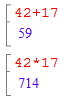
\includegraphics[width = 47pt]{images/grundrechenarten_1}\br
Möchte man mehrere Berechnungen in eine Befehlszeile schreiben, so muss man die einzelnen Befehle mit einem Semikolon trennen:\br
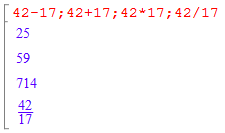
\includegraphics[width = 150pt]{images/grundrechenarten_2}\\
Möchte man hierbei die Ausgabe der Berechnung unterdrücken, verwendet man anstelle des Semikolons ein Doppelpunkt:\br
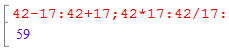
\includegraphics[width = 150pt]{images/grundrechenarten_3}

\subsection{Grundfunktionen}

\begin{tabular}{|c|c|}
\hline 
simplify(x) & Vereinfacht den Ausdruck x.\\ 
\hline 
expand(x) & Multipliziert den Ausdruck x aus. \\ 
\hline
hold(x) & Berechnet den Ausdruck x nicht. \\
\hline
sqrt(x) & Zieht die Wurzel aus dem Ausdruck x. \\
\hline
surd(x, n) & Zieht die n-te Wurzel aus dem Ausdruck x.\\
\hline
print(x.y.z) & Gibt die Ausdrücke x, y und z aus.\\
print(Unquoted, x.y.z) & Unquoted ist optional und \\ &entfernt Anführungszeichen.\\
\hline
?$<$Befehl$>$ & Zeigt Hilfe zu $<$Befehl$>$ an.\\
\hline 
\end{tabular} 
\gbr
Beispiele:\br
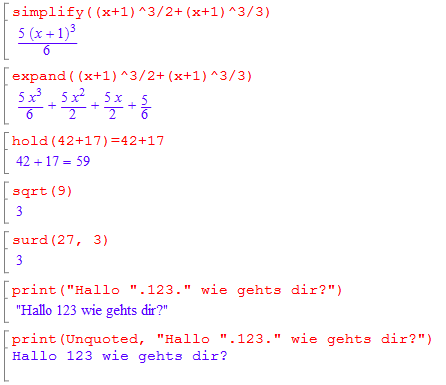
\includegraphics[width = 250px]{images/grundfunktionen_1}

\section{Vektoren und Matrizen}

Ein Vektor wird in MuPAD mit dem Befehl matrix([ ]) erzeugt.\\
Einen Vektor $\overrightarrow{x}$ = $\left(\begin{matrix}
x1\\
x2
\end{matrix}\right)$ erzeugt man folgendermaßen:\\
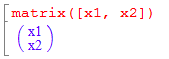
\includegraphics[width = 120px]{images/matrix_1}\br

Eine Matrix wird auf ähnliche Weise mit demselben Befehl erzeugt.\\
Eine Matrix A = $\left(\begin{matrix}
a & b\\
c & d
\end{matrix}\right)$ erzeugt man dann folgendermaßen:\\
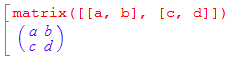
\includegraphics[width = 180px]{images/matrix_2}\br
Das heißt, innerhalb der äußeren eckigen Klammern werden die Zeilen der Matrix wieder in eckige Klammern geschrieben.

\subsection{Aufgaben}
1) Erzeugt den Vektor $\left(\begin{matrix}
5\\3\\7\\1\\
\end{matrix}\right)$ mit MuPAD.\\
2) Erzeugt die Matrix $\left(\begin{matrix}
5 & 3 & 2\\1 & 8 & 6\\7 & 9 & 4\\
\end{matrix}\right)$ mit MuPAD.

\section{Variablen und Funktionen}
\subsection{Variablen}
Variablen werden in MuPAD mit dem Operator $:=$ definiert.\\
variable := wert\\
Variablen können anschließend in Berechnungen verwendet werden.\\
Beispiel:\br
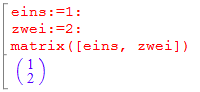
\includegraphics[width = 150px]{images/variablen_1}

\subsection{Funktionen}

Funktionen werden prinzipiell genauso vereinbart wie Variablen. Allerdings muss noch mit angegeben werden, von welchen Variablen die Funktion\\ abhängen soll:\\
$f := x --> x ^\wedge 2 * y $\\
$f2 := (x, y) --> x ^\wedge 2 * y $\\
Aufrufen kann man eine definierte Funktion dann ganz normal mit:\\
f(1), ... , f(x), ...\\
f2(1, 1), ..., f2(x, y), ...\\
Beispiele:\\
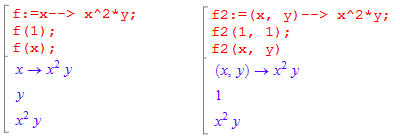
\includegraphics[width = 300px]{images/funktionen_1}

\subsection{Punkte und Listen}

Ein Punkt wird folgendermaßen erzeugt:\\
P:=[17, 42] (2-Dimensional)\\
P2:=[17, 42, 113] (3-Dimensional)\\
Auf die einzelnen Einträge eines Punktes kann zugegriffen werden:\\
P[1] = 17\\
P[2] = 42\br
Eine Liste ist eine Sammlung von Punkten und wird so erzeugt:\\
L:=[[17, 42], [3, 4], [5, 6], ..., [12, 78]]\\
Auf die einzelnen Elemente einer Liste kann man auch zugreifen:\\
L[1] = [17, 42]\\
L[1][2] = 42\\
Wie viele Elemente sich in einer Liste befinden, kann über den Befehl nops() herausgefunden werden.\br
Beispiel:\\
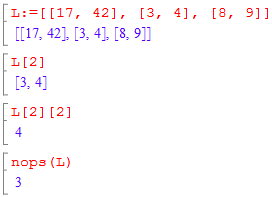
\includegraphics[width = 200px]{images/listen_1}

\subsection{Löschen}

Definierte Variablen und Funktionen können durch die Befehle delete und reset() gelöscht werden.\\
Mit dem delete-Befehl löscht man genau eine Funktion oder Variable und mit dem reset-Befehl werden alle Variablen und Funktionen zurückgesetzt.\\
Beispiele:\\
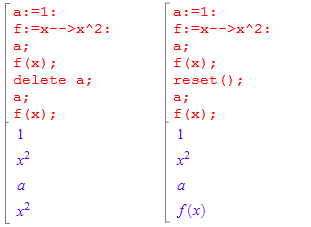
\includegraphics[width = 220px]{images/funktionen_2}

\subsection{Aufgaben}
1) Definiert drei Variablen a = 1, b=2, c=3.\\
2) Definiert eine Funktion $f(x) = x^2+3x-3$\\
3) Legt eine Liste mit 3 Punkten an.\\
\hspace*{1em} Die Punkte heißen [a, f(a)], [b, f(b)], [c, f(c)].\\
4) Gebt die zweite Koordinate von jedem Punkt aus der Liste aus.\\
5) Führt einen reset-Befehl durch.\\
6) Gebt a, b und c aus.\\
7) Gebt zweite Koordinate des zweiten Punktes der Liste aus.

\section{Differentialrechnung und Integralrechnung}

\subsection{Ableitungen}
Es gibt in MuPAD insgesamt drei Möglichkeiten eine Ableitung zu berechnen:\\
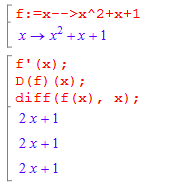
\includegraphics[width = 120px]{images/ableitungen_1}\\
f'(x) und D(f)(x) funktionieren nur vernünftig, wenn man vorher eine Funktion definiert hat. diff(f(x), x) funktioniert immer.\\
Beispiel:\\
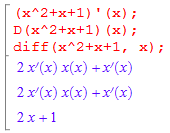
\includegraphics[width = 120px]{images/ableitungen_2}\\
Von daher ist es ratsam mit der dritten Variante zu rechnen ;)

\subsection{Integrale}
Für Integrale stellt MuPAD den Befehl int(f(x), x=a..b)\\
$\left[\int\limits_a^b f(x) dx\right]$ bereit.\\
x ist hierbei die Variable nach der integriert werden soll. Gibt man keine Integrationsgrenzen a und b an, so berechnet MuPAD die Stammfunktion F(x).
Beispiel:\\
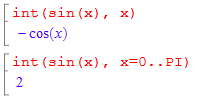
\includegraphics[width = 140px]{images/integrale_1}\\

\subsection{Aufgaben}

1) Berechnet $f'(x)$ mit $f(x) = e^{17x}\cdot sin(2x+3)$\\ 
2) Berechnet $f'(x)$ mit $f(x) = 27x^2x!+67x$\\ 
3) Berechnet das Integral $\int\limits_0^\pi x\cdot sin(x) dx $\\
4) Berechnet das Integral $\int\limits_0^\pi x^2\cdot sin(3x+1)^2 dx $\\

\section{Zeichnen}

Gezeichnet wird in MuPAD mit dem plot-Befehl. Das ganze sieht dann folgendermaßen aus:\br
\hspace*{1em}plot(\\
\hspace*{2em} plot::ArtDesPlotes(),\\
\hspace*{2em} plot::ZweiterPlot()\\
\hspace*{1em})\br
Um Maßstabstreue beim Plotten zu erhalten, kann man den Befehl ''Scaling = Constrained'' mit in den Plot schreiben:\br
\hspace*{1em}plot(\\
\hspace*{2em} plot::ArtDesPlotes(),\\
\hspace*{2em} plot::ZweiterPlot(),\\
\hspace*{2em} Scaling = Constrained\\
\hspace*{1em})\br
Hier ein Überblick über die wichtigsten Plot-Funktionen:\\

2-Dimensional: \\
\textbf{Function2d}(f(x), x=xMin..xMax)\\
\textbf{Implicit2d}(f(x)=y, x=xMin..xMax, y=yMin..yMax)\\
\textbf{Curve2d}(matrix(t), t=min..max)\\
\textbf{Point2d}([x, y])\\
\textbf{Arrow2d}(Point1, Point2)\\
\textbf{PointList2d}(list)\\

3-Dimensional: \\
\textbf{Function3d}(f(x, y), x=xMin..xMax, y=yMin..yMax)\\
\textbf{Implicit3d}(f(x, y)=z, x=xMin..xMax, y=yMin..yMax, z=zMin..zMax)\\
\textbf{Curve3d}(matrix(t, r), t=min..max, r=min..max)\\
\textbf{Point3d}([x, y, z])\\
\textbf{Arrow3d}(Point1, Point2)\\
\textbf{PointList3d}(list)\\

Beispiel:\\
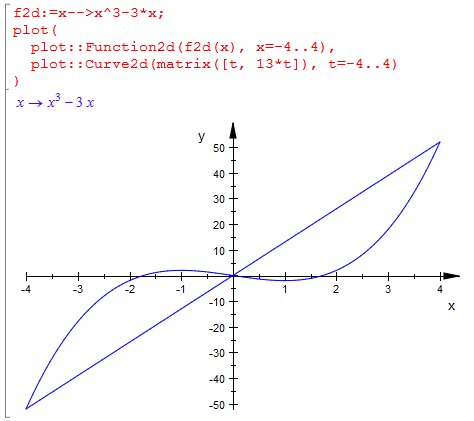
\includegraphics[width = 240px]{images/plot_1}

Gibt man den Plot-Befehlen noch weitere Parameter dazu, kann man die Art der Zeichnung weiter verändern. Mögliche Parameter sind:\\
LineStyle = [Solid, Dashed, Dotted]\\
Color = RGB::[Red, Green, Blue, Yellow, Black, ...].[transparancy (0.0-1.0)]\\
LineWidth = [0.5, 1, 1.4 , ...]\\

Beispiel:\\
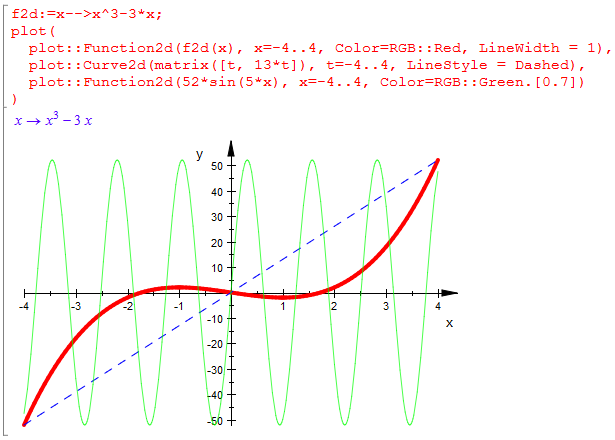
\includegraphics[width = 340px]{images/plot_2}

\subsection{Aufgaben}
1) Definiert eine Funktion $f(x) = x\cdot sin(x)$\\
2) Zeichnet die Funktion im Bereich von $-6\pi$ bis $6\pi$\\
3) Zeichnet in die selbe Zeichnung den Ausdruck $3x^2-3y^2=4$ gestrichelt und in Schwarz mit einer Transparenz von 50\% im Bereich von x=$-6\pi$ bis $6\pi$ und y=-20 bis 20.\\

\section{Programmieren}

Es ist mit MuPAD auch möglich kleine Programmier- und Kontrollstrukturen mit einzubinden.\\
Wichtige Befehle:\\

\textbf{if} (Bedingung) \textbf{then}\\
\hspace*{1em} machWas;\\
\textbf{end\_if};\\

\textbf{while} (Bedingung) \textbf{do}\\
\hspace*{1em} machWas;\\
\textbf{end\_while};\\

\textbf{for} k \textbf{from} 1 to \textbf{n} \textbf{do}\\
\hspace*{1em} machWas;\\
\textbf{end\_for};\\

\textbf{repeat}\\
\hspace*{1em} machWas;\\
\textbf{until} (Bedingung) \textbf{end\_repeat};\\

Beispiel:\\

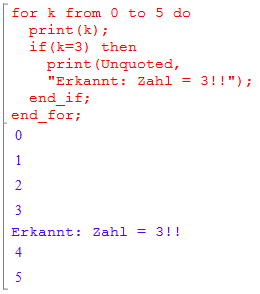
\includegraphics[width = 170px]{images/program_1}

\subsection{Aufgaben}
1) Programmiert eine while-Schleife, die alle Zahlen von 0 bis 10 ausgibt.\\
2) Prüft mit einer if-Abfrage, ob es sich um eine 7 handelt.\\
3) Macht das ganze noch einmal mit einer repeat-Schleife.\\

\chapter{Vollständige Induktion}

\section{Einleitung}
Die vollständige Induktion ist ein Beweisverfahren, bei dem man versucht zu zeigen, dass für eine Rechenvorschrift [f(n)] eine bestimmte Behauptung [B(n)] stimmt. Bei dem Verfahren wird gezeigt, dass die Bedingung für eine beliebige Zahl gilt, wenn sie auch für ihre Vorgängerzahl gilt. Findet man also eine Zahl für die die Bedingung stimmt und zeigt, dass die Bedingung auch für alle Nachfolger stimmt, so gilt automatisch, dass die Bedingung für alle Zahlen stimmt. \br
Typische Anwendungsbeispiele sind zum Beispiel:\br
		
\begin{tabular}{c l}		 
~~~~ 1. & Teileraufgaben: $ \forall n \in \N: 6 | (n^3 + 9n^2 + 26n) $ \\		  
~~~~ 2. & Summen: $ \forall n \in \N: \sum\limits_{k=1}^n (k-1)k = \dfrac{1}{3} (n+1)n(n-1) $ \\ 		
\end{tabular} 

\section{Handwerkszeug}

Binomische Lehrsätze (hier exemplarisch):\\

\begingroup
\leftskip2em 
$ (m+1)^2 = m^2+2m+1 $\\
$ (m+1)^3 = m^3+3m^2+3m+1 $\\
$ (m+1)^4 = m^4+4m^3+6m^2+4m+1 $\\
Hilfreich für Herleitung höherer Potenzen: Pascalsches Dreieck.\\
\par	
\endgroup 

Gerade / Ungerade Eigenschaften von Zahlen:\\

\begingroup
\leftskip2em 
Addition:\\
Ungerade + Ungerade = Gerade\\
Ungerade + Gerade = Ungerade\\
Gerade + Gerade = Gerade\br
Multiplikation:\\
Ungerade $\cdot$ Ungerade = Ungerade\\
Ungerade $\cdot$ Gerade = Gerade\\
Gerade $\cdot$ Gerade = Gerade\\
\par	
\endgroup 

Herausziehen des letzten Summengliedes aus einer Summe:\\

\begingroup
\leftskip2em 
$ \sum\limits_{k=1}^{n} a_{k} = \sum\limits_{k=1}^{n-1} a_{k} + a_{n} $\smallskip\\
bzw.\smallskip\\
$ \sum\limits_{k=1}^{n+1} a_{k} = \sum\limits_{k=1}^{n} a_{k} + a_{n+1} $\\
\par	
\endgroup 

\section{Herangehensweise}

\subsection*{Allgemein:}
	
Zu beweisende Aussage: $ \forall n \in \N: f(n) = B(n) $\\		
Für einen Induktionsbeweis führt man immer dieselben drei Schritte durch:\br
		
1. Anfang:\\	
		
\begingroup
\leftskip2em 
Man setzt einen Zahlenwert ein und überprüft ob die Vorschrift, die zu beweisen ist für diese Zahl stimmt. Der Einfachheit halber setzt man meistens 1 oder eine sehr kleine Zahl ein. Kommt schon in diesem Schritt nicht das erwartete Ergebnis heraus, ist der Induktionsbeweis fehlgeschlagen.\br		
$ n=1 $\\
$ f(1) = B(1) ? $\\
\par	
\endgroup 		
		
2. Annahme:\\	
	
\begingroup
\leftskip2em 
Kommt doch das gewünschte Ergebnis heraus, so nimmt man an, dass es eine Zahl m gibt, für die die Bedingung B(m) stimmt. \br
$ \exists m \in \N: f(m) = B(m) $\\
\par	
\endgroup 
		
3. Schluss:\\
			
\begingroup
\leftskip2em 
Im Schluss setzt man sowohl für die Behauptung als auch für die Rechenvorschrift für m m+1 ein.\br
$ f(m+1) = B(m+1) $\br
Um zu beweisen, dass die Behauptung nun tatsächlich für alle nachfolgenden Glieder stimmt, versucht man die Annahme [f(m) = B(m)] in f(m+1) wieder einzusetzen und anschließend zu zeigen, dass beide Seiten der Gleichung übereinstimmen. Die Strategie das zu bewerkstelligen unterscheidet sich dann natürlich von Aufgabentyp zu Aufgabentyp.
\par	
\endgroup 
\bigskip

\section{Rechenbeispiele}

Im Folgenden gibt es nun zwei Rechenbeispiele zu den oben genannten typischen Anwendungen der Induktion.		
		
\subsection{Teiler-Induktion:}
	
In diesem Aufgabentyp der Induktion geht es darum zu beweisen, dass alle Zahlen, die mit einer bestimmten Rechenvorschrift gebildet werden durch eine bestimmte Zahl teilbar sind.\br
Beispiel:\\
$ \forall n \in \N: 6 | (n^3 + 9n^2 + 26n) $\br
Anfang:\\

\begingroup
\leftskip2em 
$n=1 \colon\\
6|1^3+9 \cdot 1^2 + 26 \cdot 1 \\
6|1+9+26\\
6|36 \surd \\
$
\par	
\endgroup 
 

Annahme:\\

\begingroup
\leftskip2em 
$ \exists m \in \N: 6|m^3+9m^2+26m $\\
\par	
\endgroup 

Schluss:\\

\begingroup
\leftskip2em 
1. m+1 für m einsetzen:\\
$ 6|(m+1)^3+9(m+1)^2+26(m+1) $\br
2. Mit binomischen Formeln auflösen:\\
$ 6| m^3+3m^2+3m+1+9m^2+18m+9+26m+26 $\br
3. Annahme aus entstandenen Summanden aussortieren:\\
$ 6| \textcolor{red}{(m^3+9m^3+26m)}+3m^2+3m+1+18m+9+26 $\br
4. Für die Annahme ist ja bereits bekannt, dass Sie durch 6 teilbar ist. Gezeigt werden muss das nun nur noch für die restlichen Terme:\\
$ 6|3m^2+3m+1+18m+9+26 $\br
5. Vereinfachen:\\
$ 6|3m^2+21m+36 $\\
$ 6|3(m^2+7m+12) $\br
6. Begründung, dass $ 3(m^2+7m+12) $ immer durch 6 teilbar ist:\\
Wenn m eine gerade Zahl ist, ist $m^2+7m+12$ ebenfalls eine gerade Zahl. Ist m eine ungerade Zahl, so ist $m^2$ und 7m ungerade. Die Summe der beiden Terme ist wiederum gerade. Diese gerade Zahl plus 12 ist dann immer noch gerade.\\
(Für weitere Begründung siehe Handwerkszeug)\\
Da man aus einer geraden Zahl 2 ausklammern kann gilt nun:\\
$6 | 3 (m^2+7m+12) = 6 \left( \dfrac{m^2+7m+12}{2} \right)$\\
Der Induktionsbeweis ist also erfolgreich.
\par	
\endgroup 

\subsection{Summen-Induktion:}

Bei diesem Aufgabentyp der Induktion geht es darum, zu zeigen, dass eine Summe mit einer bestimmten Rechenvorschrift formelmäßig gelöst werden kann.\br
Beispiel:\\
$ \forall n \in \N: \sum\limits_{k=1}^n (k-1)k = \dfrac{1}{3} (n+1)n(n-1) $ \br

Anfang:\\

\begingroup
\leftskip2em 
$ n=1 \colon \sum\limits_{k=1}^1 (k-1)k = 0 \cdot 1 = (n+1)n(n-1) = (1+1) \cdot 1 \cdot (1-1)= 0 \surd $\\
\par	
\endgroup 

Annahme:\\

\begingroup
\leftskip2em 
$ \exists m \in \N \colon \sum\limits_{k=1}^m (k-1)k = \dfrac{1}{3} (m+1)m(m-1) $\\
\par	
\endgroup 

Schluss:\\

\begingroup
\leftskip2em 
1. m+1 in die Annahme einsetzen:\\
$ \sum\limits_{k=1}^{\textcolor{red}{m+1}} (k-1)k = \dfrac{1}{3} (\textcolor{red}{(m+1)}+1)\textcolor{red}{(m+1)}(\textcolor{red}{(m+1)}-1) $\smallskip\br
2. Das (m+1)te Glied aus der Summe holen(siehe Handwerkszeug):\\
$ \sum\limits_{k=1}^m (k-1)k \textcolor{red}{+ ((m+1)-1)(m+1)} = \dfrac{1}{3} (m+2)(m+1)m $\br
3. Für $ \sum\limits_{k=1}^m (k-1)k $ die Annahme einsetzen: \\
$ \textcolor{red}{\dfrac{1}{3} (m+1)m(m-1)} + m(m+1) = \dfrac{1}{3} (m+2)(m+1)m $\br
\par	
\endgroup 

4. Beide Seiten der Gleichung vereinfachen und schauen ob dasselbe herauskommt:

\begin{align*}
 \dfrac{1}{3} (m+1)m(m-1) + m(m+1)&= \dfrac{1}{3} (m+2)(m+1)m  \\
 \dfrac{1}{3} (m^2+m)(m-1) + m^2 + m &= \dfrac{1}{3} (m^2+3m+2)m  \\
 \dfrac{1}{3} (m^3 -m) + m^2 + m &= \dfrac{1}{3} (m^2+3m+2)m  \\
 \dfrac{1}{3} m^3 + m^2 + \dfrac{2}{3} m &= \dfrac{1}{3} (m^3+3m^2+2m)\\
 \dfrac{1}{3} m^3 + m^2 + \dfrac{2}{3} m &= \dfrac{1}{3} m^3 + m^2 + \dfrac{2}{3} m\\
\end{align*}

5. Induktionsbeweis ist erfolgreich:\\
$ \dfrac{1}{3} m^3 + m^2 + \dfrac{2}{3} m = \dfrac{1}{3} m^3 + m^2 + \dfrac{2}{3} m \surd $\\

\subsection{Ableitungsinduktion}

Hier geht es darum eine allgemeine Rechenvorschrift für die n-te Ableitung einer Funktion zu beweisen.\\

Beispiel:\\

$ \forall n \in \N : f^{(n)}(x) = \left( xe^{2x} \right)^{(n)} = (n+2x)\cdot 2^{n-1}\cdot e^{2x} $\\

Anfang:\\

\begingroup
\leftskip2em 
$ n=1 $\\
$ f'(x) = (1+2x)\cdot 1 \cdot e^{2x} $\\
$ f'(x) = e^{2x} + 2xe^{2x} $\\
Das stimmt!\\
\par	
\endgroup 

Annahme:\\

\begingroup
\leftskip2em 
 $ \exists m \in \N : f^{(m)}(x) = (m+2x)\cdot 2^{m-1}e^{2x} $\\
\par	
\endgroup 

Schluss:\\

\begingroup
\leftskip2em 
(m+1) in die Annahme einsetzen:\\
$ f^{(m+1)}(x) = (m+1+2x)\cdot 2^m \cdot e^{2x} $\\
$ f^{(m+1)}(x) = m 2^m e^{2x} + 2x2^me^{2x} + 2^me^{2x} $\\

Versuchen denselben Ausdruck durch Ableiten der Annahme herzuleiten:\\
$ f^{(m)}(x) = (m+2x)\cdot 2^{m-1} e^{2x} $\\
$ f^{(m+1)}(x) = \left( m 2^{m-1} e^{2x} + 2x 2^{m-1} e^{2x} \right)' $\\
$ f^{(m+1)}(x) = m 2^{m} e^{2x} + 2x 2^{m} e^{2x} + 2^m e^{2x} $\\

Die beiden Ausdrücke sind identisch.\\
Induktion war erfolgreich.\\
\par	
\endgroup 

\newpage	
\section{Übungsaufgaben}

\subsection*{Aufgabe 1:}

Beweisen Sie durch Induktion für alle natürlichen Zahlen n:\\
\hspace*{2em}$ 10^n + 18n -28 $ ist durch 27 teilbar.

\subsection*{Aufgabe 2:}
Beweisen Sie durch Induktion für 
alle natürlichen Zahlen n:\\
\hspace*{2em}$ \sum\limits_{k=1}^n \dfrac{1}{\sqrt{k}} \geq \sqrt{n} $

\subsection*{Aufgabe 3:}
Beweisen Sie durch Induktion für alle natürlichen Zahlen n:\\
\hspace*{2em}$ n^6+10n^4+4n^2 $ ist durch 15 teilbar.

\subsection*{Aufgabe 4:}
Beweisen Sie durch Induktion für alle natürlichen Zahlen n:\\
\hspace*{2em}$ n^3 - n $ ist durch 6 teilbar.

\subsection*{Aufgabe 5:}
Beweisen Sie durch Induktion für alle natürlichen Zahlen n:\\
\hspace*{2em}$ \sum\limits_{k=1}^n \dfrac{k}{2^k} = 2- \dfrac{n+2}{2^n} $

\subsection*{Aufgabe 6:}
Beweisen Sie durch Induktion für alle natürlichen Zahlen n:\\
\hspace*{2em}$ n^7 - n $ ist durch 7 teilbar.

\subsection*{Aufgabe 7:}
Beweisen Sie durch Induktion für alle natürlichen Zahlen n:\\
\hspace*{2em}$ \sum\limits_{k=1}^{n+1} (2k-1)^2 = \dfrac{1}{3} (4n^3+12n^2+11n+3) $

\subsection*{Aufgabe 8:}
Beweisen Sie durch Induktion für alle natürlichen Zahlen n:\\
\hspace*{2em}$ 9^n + 7 $ ist durch 8 teilbar.

\chapter{Trigonometrie}
Okay, das folgende Kapitel wird eher langweilig werden, ist für das mathematische Grundverständnis allerdings unabdingbar. Mit trigonometrischen Funktionen wie Sinus, Kosinus und Tangens umgehen zu können ist für den weiteren Verlauf des Studiums sehr hilfreich ;).

\section{Grundbegriffe}
Eine $2\pi$-periodische Funktionen (Sinus und Kosinus) kann man charakterisieren durch bestimmte Eigenschaften.\\
Diese Eigenschaften sind die Amplitude a, die Periode p der Funktion und der Nullphasenwinkel $\varphi_0$.\\

\subsection{Amplitude}
Die Amplitude gibt den maximalen Ausschlag einer Funktion an.\\
Die Amplitude ist die Strecke von dem Mittelwert der Funktionskurve bis zum höchsten ODER bis zum tiefsten Ausschlag.\\
Die Strecke vom höchsten bis zum tiefsten Ausschlag entspricht genau dem Doppelten der Amplitude.
\begin{center}
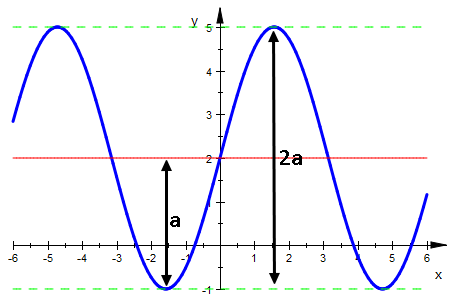
\includegraphics[width=200pt]{images/amplitude_1}
\end{center}
\subsection{Periode}
Die Periode p gibt an, nach welchem Intervall sich die Funktion anfängt zu wiederholen.
\begin{center}
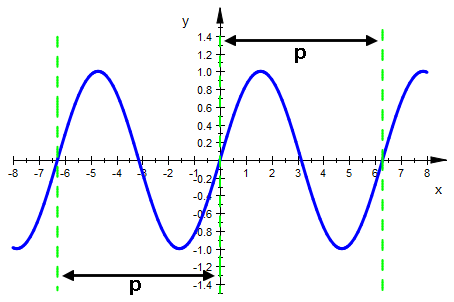
\includegraphics[width=200pt]{images/amplitude_2}\\
\end{center}
\subsection{Nullphasenwinkel}
Mann kann eine Trigonometrische Funktion durch das einbauen eines Nullphasenwinkels nach links bzw. nach rechts verschieben. 
\begin{center}
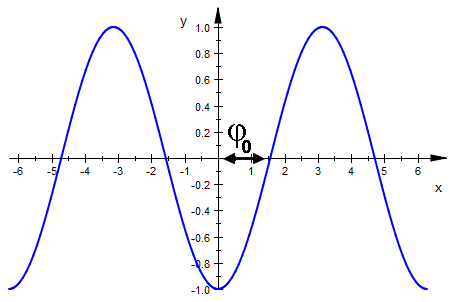
\includegraphics[width=200pt]{images/nullphase_1}\\
\end{center}
\section{Funktionen modellieren}
Das Aussehen einer trigonometrischen Funktion kann komplett durch diese drei Eigenschaften modelliert werden. Da für die Sinus- und die Kosinusfunktion alle Dinge genau analog funktionieren, gibt es an dieser Stelle nur ein Beispiel für die Sinusfunktion.
\subsection{Sinusfunktion}
Bedeutung von Amplitude, Periode und Nullphasenwinkel gezeigt anhand der Sinusfunktion:\\
$ f(x) = a \cdot \sin((\dfrac{2\pi}{p}\cdot x)-\varphi_0) $\\

Eine Verschiebung entlang der X-Achse kann auch direkt erfolgen, wobei der Graph dann um $x_0$ Einheiten nach links / rechts verschoben wird.\\
$ f(x) = a \cdot \sin(\dfrac{2\pi}{p}\cdot (x-x_0)) $\\

1. Fall:\\
$ a=5, p=2\pi, \varphi_0=0$\\
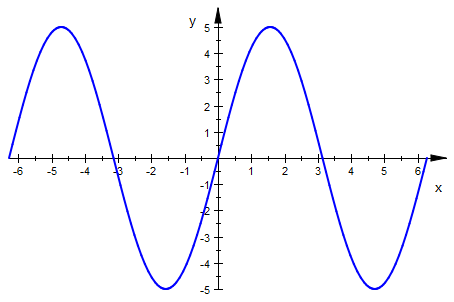
\includegraphics[width=250pt]{images/sinus_1}\\

2. Fall:\\
$ a=3, p=25, \varphi_0=\pi$\\
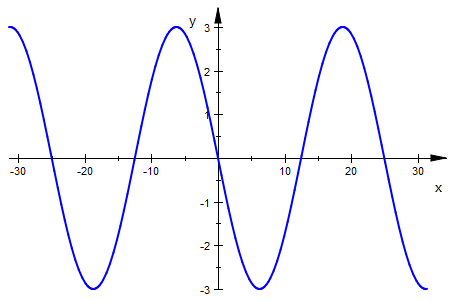
\includegraphics[width=250pt]{images/sinus_2}\\

\subsection{Aufgabe}
Modelliert eine Sinusfunktion für den Sonnenstand.\\
Die Einheiten der X-Achse sollen Stunden und die der Y-Achse Grad sein.\\
Die Zeit zwischen einem Sonnenaufgang und dem nächsten beträgt 24 Stunden.\\
Die Sonne erreicht bei 60 Grad ihren höchsten Stand.\\
Zum Zeitpunkt x=6 Stunden geht die Sonne zum ersten Mal auf.\\

\section{Rechenregeln mit trigonometrischen Funktionen}
\subsection{Identitäten}
$ \sin^2(x) + \cos^2(x) = 1 $\\
$ \tan(x) = \dfrac{\sin(x)}{\cos(x)} $\\
\subsection{Additionstheoreme}
$\sin(x+y) = \sin(x)\cos(y) + \sin(y)\cos(x)$\\
$\sin(x-y) = \sin(x)\cos(y) - \sin(y)\cos(x)$\\
$\cos(x+y) = \cos(x)\cos(y) - \sin(x)\sin(y)$\\
$\cos(x-y) = \cos(x)\cos(y) + \sin(x)\sin(y)$\\
$\tan(x+y) = \dfrac{\sin(x+y)}{\cos(x+y)}$\\
$\tan(x-y) = \dfrac{\sin(x-y)}{\cos(x-y)}$\\
\subsection{Lösungen von trigonometrischen Gleichungen}
Da die trigonometrischen Funktionen alle periodisch sind, gibt es für die Lösung einer trigonometrischen Gleichung immer unendlich viele Lösungen.\\
Beispiel:\\
$ 5*\sin(x) = 5$\\
$ \Rightarrow \sin(x) = 1 $\\
Nach erster Überlegung kommt man schnell auf: \\
$ x = \dfrac{\pi}{2} $\\
Da der Sinus allerdings eine $2\pi$-periodische Funktion ist, gilt die Lösung auch für alle Punkte, die ein $2\pi$-faches von dem gefundenen Punkt entfernt sind. Geschrieben wird das ganze dann so:\\
$ x = \dfrac{\pi}{2} + 2\pi\cdot k, k\in\Z $\\

\newpage
\section{Wofür brauch ich jetzt den ganzen Kram für später?! - Anwendungen und Aufgaben}

\subsection{MPHY: Schwingungen}

Direkt aus einer Physik-Probeklausur:\\

(1) Eine Masse von 20g hängt an einer masselosen Feder und dehnt sie dadurch um 6cm aus. Geben Sie Ihre Lage zu jeder beliebigen Zeit an, wenn sie zur Zeit t=0 um 2cm herabgezogen und losgelassen wurde. Geben Sie Amplitude, Periode und Frequenz der Schwingung an. geben Sie die Ortsfunktion der Masse an. Vernachlässigen Sie Reibungseffekte.\\

Hinweis: Periode p berechnet sich durch:\\
$ p= 2\pi\cdot\sqrt{\dfrac{\text{Ausdehnung in Ruhelage}}{9.81}} $\\

Ansatz für Ortsfunktion:\\
$ f(x) = a \cdot \sin((\dfrac{2\pi}{p}\cdot x)-\varphi_0) $\\

\subsection{ANA2: Koordinaten-Transformation}

Bei bestimmten Aufgaben im Rahmen der Analysis II - Vorlesung kommen Aufgaben vor, bei denen in bestimmten Gleichungen x und y mit Polarkoordinaten ersetzt werden und anschließend der entstehende Ausdruck nach dem Radius aufgelöst werden muss.\\
Also $\left(\begin{matrix}x\\y\\\end{matrix}\right) = \left(\begin{matrix}r\cdot\sin(\varphi)\\r\cdot\cos(\varphi)\\\end{matrix}\right)$\gbr
Aufgaben: Ersetzte in den Gleichungen x und y wie oben genannt und löse den Ausdruck nach r auf:\\

\begingroup
\leftskip2em 
1) $y=3x-5$\\
2) $-y^2 = x^2-9$\\
3) $xy = x^2+y^2+25$\\
\par	
\endgroup 

\subsection{ANA1: Komplexe Zahlen}

Das ist das Bestandteil der nächsten Stunde und wir werden uns hier jetzt damit noch nicht befassen.\\

\subsection{Weitere Aufgaben:}

1) Zeigen Sie, dass gilt:

\begingroup
\leftskip2em 
$ cos^2(x)-sin^2(x) = 1-2\cdot sin^2(x) $\\
\par	
\endgroup 

2) Zeigen Sie, dass gilt:

\begingroup
\leftskip2em 
$ \sqrt{\dfrac{1+sin(x)}{1-sin(x)}} = \dfrac{1+sin(x)}{|cos(x)|} $\\
\par	
\endgroup 

3) Geben Sie alle Lösungen für folgende Gleichungen an:

\begingroup
\leftskip2em 
$ 2\cdot cos(x) -1 = 0 $\\
\par	
\endgroup 

4) Geben Sie alle Lösungen für folgende Gleichungen an:

\begingroup
\leftskip2em 
$ tan(x)\cdot sin^2(x) = 2\cdot tan(x) $\\
\par	
\endgroup 

5) Leiten Sie mittels der Additionstheoreme neue Ausdrücke für folgende Terme her:

\begingroup
\leftskip2em 
a) $sin(2\alpha) = ?$\\
b) $cos(2\alpha) = ?$\\
c) $tan(2\alpha) = ?$\\
\par	
\endgroup 

6) Löst mit den errechneten ausdrücke die Gleichungen für:

\begingroup
\leftskip2em 
$sin(\alpha) = \dfrac{3}{5} $ und $cos(\alpha) = ?$\\
\par	
\endgroup 

\chapter{Komplexe Zahlen}

\section{Einleitung}

Die komplexen Zahlen ($\C$) sind eine Erweiterung des Zahlenraumes der reellen Zahlen ($\R$). Jede Zahl ist in $\C$ definiert durch einen Realteil und einem Imaginärteil.\\
$ z \in \C \colon z = x + iy$\\
Das i ist die so genannte imaginäre Einheit, und zeigt an, dass der Wert, der mit dem i zusammensteht zum Imaginärteil gehört.\\
Das Besondere an der imaginären Einheit ist, dass für sie bestimmte Rechenregeln gelten:\\
$ i^2 = -1 $, also $ \sqrt{-1} = i$\\
Durch die komplexen Zahlen wird somit auch das Wurzelziehen aus negativen Termen möglich gemacht:\\
$ \sqrt{-16} = \sqrt{16 \cdot -1} = \sqrt{16} \cdot \sqrt{-1} = 4i $\\

\section{Darstellungsformen}

Die komplexen Zahlen lassen sich in drei Darstellungsformen beschreiben:\\
In kartesische Koordinaten, als e-Funktion und in Polarkoordinaten.\\
Jede dieser Darstellungsformen hat seine eigenen Rechenvorzüge und es ist von großem Vorteil wenn man sicher und schnell zwischen den Formen hin und her rechnen kann.\\

\subsection*{Kartesische Darstellungsform}
	$z = x + iy$\\
\subsection*{Eulersche Darstellungsform}
	$z=|z|\cdot e^{i \cdot \arg(z)}$
\subsection*{Darstellung in Polarkoordinaten}
	$z=|z|\cdot (\cos(\arg(z)) + i\sin(\arg(z)))$
	
\section{Handwerkszeug}
Definitionen:\\

\begingroup
\leftskip2em 
$ z=x+iy \in \C $\\
$ \Im(z) = $Imaginärteil$(z) = y $\\
$ \Re(z) = $Realteil$(z) = x $\\
$ |z| = $ Betrag $(z) = \sqrt{\Re(z)^2+\Im(z)^2}=\sqrt{x^2+y^2} $\\
$ \overline{z} = \text{z konjugiert komplex} = x-iy $\\
$
\varphi = \arg(z) = $Argument$(z) = \left\{
\begin{array}{l}
\arctan \frac{y}{x}, x>0, y $ beliebig$\\ 
\arctan \frac{y}{x} + \pi, x<0, y\geq 0\\
\arctan \frac{y}{x} - \pi, x<0, y< 0\\
\dfrac{\pi}{2}, x=0,y>0\\
-\dfrac{\pi}{2}, x=0, y<0\\
$unbestimmt$, x=0, y=0
\end{array}
\right.\\
$
\par	
\endgroup 

Rechenregeln:\\

\begingroup
\leftskip2em 
$ i^2 = -1 $\\
$ |a \cdot b| = |a| \cdot |b| $\\
$\left| \dfrac{a}{b} \right| = \dfrac{|a|}{|b|} $\\
$ z\cdot\overline{z}=|z|^2 = \Re(z)^2+\Im(z)^2$\\
$ z+\overline{z}=2\Re(z) $\\
$ z-\overline{z}=2i\Im(z) $\\
\par	
\endgroup 

Rechnen mit der e-Funktion:\\

\begingroup
\leftskip2em 
$ r\cdot e^{ix} = r(\cos(x) + i\sin(x)) $\\
$ e^a \cdot e^b = e^{a+b} $\hspace{2em}
$ \dfrac{e^a}{e^b} = e^{a-b} $\hspace{2em}
$ (e^a)^b = e^{a \cdot b} $\\
$ \Re(r\cdot e^{ix}) = r \cdot \cos(x) $\hspace{2em}
$ \Im(r\cdot e^{ix}) = r \cdot \sin(x) $ \\
\par	
\endgroup 

\section{Einfache Übungen}
\subsection{Addition \& Subtraktion}
\begingroup
\leftskip2em 
a) $(3+4i) - (5+3i)= ?$\\
b) $(4+6i) + \overline{(7+6i)}= ?$\\
c) $(3+4i) + i= ?$\\
d) $(2-2i) - \overline{(2-2i)}= ?$
\par	
\endgroup 
\subsection{Multiplikation \& Division}
\begingroup
\leftskip2em 
a) $(2+2i)\cdot(3+7i)= ?$\\
b) $4i\cdot (3+2i) \cdot 2= ?$\\
c) $50i / 25i= ?$\\
d) $(25+25i) / (5+5i)= ?$
\par	
\endgroup 
\subsection{In eulersche Darstellungsform umwandeln}
\begingroup
\leftskip2em 
a) $(2+4i) = ?$\\
b) $ 2\cdot(\cos(\pi)+i\sin(\pi)) = ?$ \\
c) $(i\cos(\pi/4)+\sin(\pi/4))= ? $\\
d) $(7+11i) = ?$
\par	
\endgroup 
\subsection{Weitere Aufgaben}
\begingroup
\leftskip2em 
a)$\Re(5 / (3+2i)) = ?  $\\
b)$\Im((3i+2) / (3+2i)) = ?  $
\par	
\endgroup 

\section{Herangehensweise}

Im allgemeinen ist es ratsam zu versuchen möglichst alles, was man mit komplexen Zahlen berechnen soll in der \textbf{eulerschen Darstellungsform} zu berechnen, da es für diese einige sehr bequeme Rechenregeln gibt.\\
\text{[}Das gilt insbesondere für Wurzeln und Potenzen etc.]\br

\textbf{Durch eine komplexe Zahl teilen:} \\
Um durch eine komplexe Zahl zu teilen erweitert man Zähler und mit dem konjugiert Komplex der Zahl. Dadurch erhält man einen rein reellen Nenner und kann gegebenenfalls einfacher weiter rechnen.\\
$ \dfrac{a}{z} = \dfrac{a\cdot\overline{z}}{z\cdot\overline{z}}=\dfrac{a\cdot\overline{z}}{\Re(z)^2+\Im(z)^2} $\br

\textbf{Wurzeln aus komplexen Zahlen ziehen:}\\
Wird auch am besten in der eulerschen Darstellungsform durchgeführt, da gilt:\\
$\sqrt[a]{e^{i\arg(z)}} = (e^{i\arg(z)})^{\dfrac{1}{a}} = (e^{i\arg(z)+2k\pi})^{\dfrac{1}{a}} = e^{\dfrac{\arg(z)+2k\pi}{a}}, k=0..(a-1)$\\
Zu beachten ist hierbei, dass mehrere Lösungen entstehen, da man, wenn man ein Vielfaches von $2\pi$ zum Argument von z hinzuzählt wieder dieselbe komplexe Zahl erhält.

\section{Rechenbeispiele}

\subsection*{Beispiel 1:}

Berechnen Sie Realteil, Imaginärteil, Argument und Betrag der folgenden komplexen Zahl:\\
\hspace*{3em} $ z = \dfrac{\left[  2\cdot (\cos(\dfrac{\pi}{12})+i\sin(\dfrac{\pi}{12}))\right]^7}{\left[  4\cdot (\cos(\dfrac{\pi}{4})+i\sin(\dfrac{\pi}{4}))\right]^3} $\br
Erkennen: Komplexe Zahlen sind gegeben in Polardarstellung.\\
Umwandeln in eulersche Darstellungsform:\\
\hspace*{3em} $ z = \dfrac{\left[  2\cdot e^{\dfrac{i\pi}{12}}\right]^7}{\left[  4\cdot e^{\dfrac{i\pi}{4}}\right]^3} $\br
Nach Potenzgesetzen vereinfachen:\\
\hspace*{3em} $ z = \dfrac{  2^7\cdot e^{i\dfrac{7\pi}{12}}}{4^3\cdot e^{i\dfrac{3\pi}{4}}} $\\
\hspace*{3em} $ z =  2\cdot e^{-i\dfrac{\pi}{6}} $\gbr
Lösung:

\begingroup
\leftskip3em 
$ \Re(z) = 2\cdot\cos(\dfrac{\pi}{6}) $\\
$ \Im(z) = 2\cdot\sin(\dfrac{\pi}{6}) $\\
$ arg(z) = -\dfrac{\pi}{6} $\\
$ | z |  = 2 $
\par	
\endgroup 


\subsection*{Beispiel 2:}
Für welche komplexen Zahlen z gilt die Gleichung

\begingroup
\leftskip3em 
$ \Im\left( \dfrac{z^2}{\overline{z}+z} \right) = 2 $?
\par	
\endgroup 
Skizzieren Sie die Lösungsmenge!\br
Ansatz:\\
\hspace*{3em}$z=x+iy$\br
Rechnung:

\begingroup
\leftskip3em 
$ \Im\left( \dfrac{(x+iy)^2}{(x-iy)+(x+iy)} \right) = 2 $\\
$ \Im\left( \dfrac{x2+2ixy-y^2}{2x} \right) = 2 $\\
$ \dfrac{2xy}{2x} = 2 $\\
$ y = 2$\\
\par	
\endgroup 
Skizze der Lösungsmenge:\\
\hspace*{3em}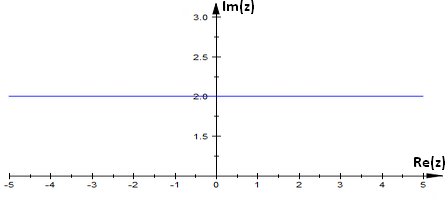
\includegraphics[width=200pt]{images/complex_numbers_01.png}\br
Antwort:

\begingroup
\leftskip3em 
Die Gleichung gilt für alle komplexen Zahlen deren Imaginärteil 2 ist.\\
\par	
\endgroup 

\newpage
\section{Übungsaufgaben}
\subsection*{Aufgabe 1:}
Bestimmen Sie alle komplexen Zahlen $ z \in\C$, die der Ungleichung\\
\hspace*{3em}$|z|<|z+3|$\\
genügen. Skizzieren Sie die Lösungsmenge.
\subsection*{Aufgabe 2:}
Berechnen Sie alle $a\in\R$ und $b\in\R$, für die\\
\hspace*{3em}$ e^{a+ib} = 1+i\sqrt{3}$\\
gilt.
\subsection*{Aufgabe 3:}
Berechnen Sie alle komplexen Zahlen z, die der Gleichung\\
\hspace*{3em}$ z^5 = \dfrac{1+i}{e^{i\dfrac{\pi}{2}}}(\cos(1)+i\sin(1))$\\
genügen.
\subsection*{Aufgabe 4:}
Bestimmen Sie alle komplexen Zahlen $ z \in\C$, die der Ungleichung\\
\hspace*{3em}$2\Re(z) + \Im(z)\leq |z|^2$\\
genügen. Skizzieren Sie die Lösungsmenge.
\subsection*{Aufgabe 5:}
Berechnen Sie alle komplexen Zahlen z, die der Gleichung\\
\hspace*{3em}$ \left( \dfrac{1+i}{z^2} \right)^2 = \dfrac{1-i}{e^{i\dfrac{\pi}{4}}}$\\
genügen.
\subsection*{Aufgabe 6:}
Bestimmen Sie alle komplexen Zahlen $ z \in\C$, die der Gleichung\\
\hspace*{3em}$\left| \dfrac{3+4i}{z-i} \right| = 5$\\
genügen. Skizzieren Sie die Lösungsmenge.

\chapter{Grenzwerte}

\section{Einleitung}

Als Grenzwert wird der Wert bezeichnet, den eine Funktion an einer ganz bestimmten Stelle annimmt.\\
Für Rechnungen am interessantesten sind meist Grenzwerte, wo die x-Werte gegen 0 oder $\infty$ gehen.\\

\section{Handwerkszeug}

\subsection*{Regel von l'Hôspital}

\begingroup
\leftskip2em 
Wenn folgende Situation auftritt:\br
$ \lim\limits_{x\to a} \dfrac{f(x)}{g(x)} = \dfrac{0}{0} \text{ oder } \dfrac{\infty}{\infty} $\br
Und wenn f(x) und g(x) differenzierbare Funktionen sind, dann gilt nach der Regel von l'Hôspital:\br
$ \lim\limits_{x\to a} \dfrac{f(x)}{g(x)} = \lim\limits_{x\to a} \dfrac{f'(x)}{g'(x)} $\br
Man darf in einer solchen Situation also einfach Zähler und Nenner getrennt von einander differenzieren und versuchen den Grenzwert erneut zu bilden.\bigskip\medskip\\
Bei folgender Situation:\\
$ \lim\limits_{x\to a} f(x) = 0 $ und $ \lim\limits_{x\to a} g(x) = \infty $\\
also $ \lim\limits_{x\to a} f(x)\cdot g(x) = {0}\cdot{\infty} \Rightarrow $ undefiniert(!)\\
kann man den Term künstlich in die passende Form für l'Hôspital bringen:\\
$ \lim\limits_{x\to a} \dfrac{f(x)}{\dfrac{1}{g(x)}} = \dfrac{0}{0}$\\
\par	
\endgroup 

\subsection*{Potenzen umwandeln mit Hilfe der e-Funktion}

\begingroup
\leftskip2em 
$ a^x = e^{x \cdot \ln(a)} $\\
$ \Rightarrow f(x)^{g(x)} = e^{g(x) \cdot \ln(f(x))} $\br
$ \text{z.B.: } \sin(x)^{\cos(x)} = e^{\cos(x) \cdot \ln(\sin(x))}$\\
\par	
\endgroup 

\subsection*{Wer gewinnt gegen wen?}

Nicht alle Funktionen nähern sich gleich schnell an wenn man im Grenzwert gegen einen Wert geht.\\
Hier sind einmal die wichtigsten Funktionstypen ihrer ''Schnelligkeit'' nach sortiert:\\
(Schnellste zuerst)\\

\begingroup
\leftskip2em 
1. Fakultäten\\
2. Exponentialfunktionen\\
3. Potenzfunktionen\\
4. Lineare Funktionen\\
5. Logarithmische Funktionen\\\

\par	
\endgroup 

Als Beispiel: \\
Für $ \lim\limits_{x\to 0+} x \cdot \ln(x) = a$ ist zunächst einmal nicht ganz klar was für a herauskommt, da $ \lim\limits_{x\to 0+} x = 0 $ und $ \lim\limits_{x\to 0+} \ln(x) = -\infty$. Da lineare Funktionen allerdings schneller im Grenzwert gegen einen Wert gehen, gewinnt das x und es gilt a=0.\\

\subsection*{Ein paar einfache Grenzwerte:}

$\lim\limits_{x\to\infty} \dfrac{1}{x} = 0$ und $\lim\limits_{x\to 0} \dfrac{1}{x} = \infty$\br
$\lim\limits_{x\to \infty} x\cdot e^{-x} = 0$ und $\lim\limits_{x\to 0} x\cdot e^{-x} = 0$\\

\subsection*{Bei einem Bruch zweier Polynome p(x) und q(x) gilt:}
$\lim\limits_{x\to\infty} \dfrac{p(x)}{q(x)} = 0$, wenn Grad q(x) $>$ Grad p(x).\br
$\lim\limits_{x\to\infty} \dfrac{p(x)}{q(x)} = \infty$, wenn Grad q(x) $<$ Grad p(x).\br
$\lim\limits_{x\to\infty} \dfrac{p(x)}{q(x)} = $ [Quotient der Höchstkoeffizienten], wenn\\
\hspace*{6em}Grad q(x) $=$ Grad p(x).\\

\section{Herangehensweise}
1. Substitution.\br
\hspace*{2em}$ n^m = \dfrac{1}{x} \Rightarrow \lim\limits_{n\to\infty} \dfrac{a}{n^m} = \lim\limits_{x\to 0} ax $\br
2. Funktion ist in exponentieller Form ($a^b$).\\

\begingroup
\leftskip2em 
Mit den Rechenregeln für Potenzen in e-Funktion umwandeln. Anschließend kann man für die Grenzwertbetrachtung nur den Exponenten verwenden und ganz am Schluss den herausbekommenen Grenzwert wieder in die e-Funktion einsetzen.\\
\par	
\endgroup 

3. Versuchen Funktion in Form für die Regel von l'Hôspital zu bringen.\\

\begingroup
\leftskip2em 
Anschließend die Regel von l'Hôpital so lange anwenden, bis nicht mehr die Situation $ \dfrac{0}{0} \text{ oder } \dfrac{\infty}{\infty} $ auftritt.\\
\par	
\endgroup 

4. Grenzwert berechnen.\\

\begingroup
\leftskip2em 
Hierbei beachten, welche Arten von Funktionen gegen welche anderen Funktionen im Grenzwert dominieren und welche nicht. Bei einem Bruch lohnt es sich oftmals Zähler und Nenner durch den Term zu teilen, der am schnellsten wächst, um sehen zu können, was der Grenzwert ist.\\
\par	
\endgroup 

\section{Rechenbeispiele}
\subsection*{Beispiel 1: }
Gibt es Werte für $\alpha, \beta, \gamma \in\R$, so dass \\
\hspace*{2em}$ \lim\limits_{n\to\infty} n\cdot\left( e^{\dfrac{\alpha}{n}}- e^{\dfrac{-\beta}{n}}\right) = \gamma $?\br
1. Substitution [$ n=\dfrac{1}{x} $]:\\
\hspace*{2em}$ \lim\limits_{x\to 0} \dfrac{e^{{\alpha}{x}}- e^{{-\beta}{x}}}{x} = \gamma $\br
3. Anwenden der Regel von l'Hospital:\\
\hspace*{2em}$ \lim\limits_{x\to 0} \alpha{e^{{\alpha}{x}}+\beta e^{{-\beta}{x}}} = \gamma $\br
4. Grenzwert berechnen:\\
\hspace*{2em}$ \alpha + \beta = \gamma $\br
\textbf{Antwortsatz:}\\
Der Grenzwert gilt für alle $\alpha, \beta, \gamma \in\R$, solange wie $ \alpha + \beta = \gamma $.

\subsection*{Beispiel 2: }
Gibt es Werte für $ a\in\R$, so dass \br
\hspace*{2em}$ \lim\limits_{n\to\infty} (\cos(\dfrac{a}{n}))^{\dfrac{1}{1-\cos(\dfrac{1}{n})}} = \dfrac{1}{2}$?\gbr
1. Substitution [$ n=\dfrac{1}{x} $]:\br
\hspace*{2em}$ \lim\limits_{x\to 0} (\cos({a}{x}))^{\dfrac{1}{1-\cos({x})}}= \dfrac{1}{2}$\br
2. Funktion ist in exponentieller Form ($a^b$). $\Rightarrow$ in e-Funktion umschreiben:\br
\hspace*{2em}$ \lim\limits_{x\to 0} e^{\dfrac{\ln(\cos({a}{x}))}{1-\cos({x})}}= \dfrac{1}{2}$\br
Vorerst nur Exponenten betrachten.\br
\hspace*{2em}$ \lim\limits_{x\to 0} {\dfrac{\ln(\cos({a}{x}))}{1-\cos({x})}}= ? \hspace*{1em} \Rightarrow \text{Fall:}\dfrac{0}{0}$\br
3. Regel von l'Hospital anwenden.\br
\hspace*{2em}$ \lim\limits_{x\to 0} {\dfrac{-a\cdot \sin(ax)}{\cos(ax)\cdot\sin(x)}}= ? \hspace*{1em} \Rightarrow \text{Fall:}\dfrac{0}{0}$\br
4. Regel von l'Hospital erneut anwenden.\br
\hspace*{2em}$ \lim\limits_{x\to 0} {\dfrac{-a^2\cdot \cos(ax)}{-a\sin(ax)\sin(x)+\cos(ax)\cos(x)}}= -a^2$\br
5. Grenzwert zurück in e-Funktion einsetzen.\\

\begingroup
\leftskip2em 
$e^{-a^2}=\dfrac{1}{2} \Rightarrow -a^2=\ln(\dfrac{1}{2}) \Rightarrow a=\pm\sqrt{-\ln(\dfrac{1}{2})}$
\par	
\endgroup 

\newpage
\section{Übungsaufgaben}

\subsection*{Aufgabe 1: }
Gibt es Werte für $\alpha, \beta, \gamma \in\R$, so dass \br
\hspace*{2em}$ \lim\limits_{n\to\infty} n^2\cdot\left( e^{\dfrac{\alpha}{n^2}}- e^{\dfrac{-\beta}{n^2}}\right) = \gamma $?
\subsection*{Aufgabe 2: }
Gibt es Werte für $ a\in\R$, so dass \br
\hspace*{2em}$ \lim\limits_{n\to\infty} (\cos(\dfrac{a}{n^2}))^{\dfrac{1}{1-\cos(\dfrac{1}{n^2})}} = \dfrac{1}{2}$?
\subsection*{Aufgabe 3: }
a und b seien positive reelle Zahlen. Berechnen Sie \br
\hspace*{2em}$ \lim\limits_{n\to\infty} (\arctan(\dfrac{a}{n}))^{{\sin(\dfrac{1}{n})}}$\br
oder begründen Sie, dass der Grenzwert nicht existiert.
\subsection*{Aufgabe 4: }
Gibt es Werte für $ a\in\R$, so dass \br
\hspace*{2em}$ \lim\limits_{n\to\infty} (\cos(\dfrac{a}{n}))^{n^2} < \dfrac{1}{2}$?
\subsection*{Aufgabe 5: }
Gibt es Werte für $ a\in\R$, so dass \br
\hspace*{2em}$ \lim\limits_{n\to\infty} n^3(\cos(\dfrac{a}{n^3})-1) = 3$?
\subsection*{Aufgabe 6: }
Gibt es eine Zahl $ a\in\R$, so dass \br
\hspace*{2em}$ \lim\limits_{n\to\infty} (1+\sin(\dfrac{a}{n}))^{{\arctan(\dfrac{1}{n})}} = 17$\br
gilt? Wenn ja, berechnen Sie a. Wenn nein, begründen Sie die Nicht-Existenz.\\

\chapter{Folgen und Reihen}

\section{Einleitung}
Der Umgang mit Folgen und Reihen ist ein sehr wichtiges Handwerkszeug in der Analysis.\\
Vor allem geht es hierbei darum, herauszufinden, ob eine Reihe gegen einen bestimmten Wert konvergiert oder einfach unendlich groß/klein wird.\br

\section{Handwerkszeug}

\subsection*{Allgemeinformen}

Reihen:

\begingroup
\leftskip2em 
$ \sum\limits_{n=0}^\infty a_n$\\
\par	
\endgroup 

Alternierende Reihen:

\begingroup
\leftskip2em 
$ \sum\limits_{n=0}^\infty (-1)^n a_n$\\
\par	
\endgroup 

Potenzreihen:

\begingroup
\leftskip2em 
$ \sum\limits_{n=0}^\infty a_n (x-x_0)^n$\\
\par	
\endgroup 

\subsection*{Konvergenzkriterien}
Quotientenkriterium:\\

\begingroup
\leftskip2em 
$  \lim\limits_{n\to\infty} \left| \dfrac{a_{n+1}}{a_{n}} \right|\hspace{1em}
\left\{
\begin{array}{l}
<1 \Rightarrow \text{konvergent}\\ 
=1 \Rightarrow \text{Raabe-Kriterium versuchen}\\
>1 \Rightarrow \text{divergent}\\
\end{array}
\right.
$\br
\par	
\endgroup 

Wurzelkriterium:\\

\begingroup
\leftskip2em 
$  \lim\limits_{n\to\infty} \sqrt[n]{|a_n|}\hspace{1em}
\left\{
\begin{array}{l}
<1 \Rightarrow \text{konvergent}\\ 
=1 \Rightarrow \text{Raabe-Kriterium versuchen}\\
>1 \Rightarrow \text{divergent}\\
\end{array}
\right.
$\\
\par	
\endgroup 

Raabe-Kriterium:\\

\begingroup
\leftskip2em 
$  \lim\limits_{n\to\infty} n \left( 1- \dfrac{a_{n+1}}{a_{n}} \right)\hspace{1em}
\left\{
\begin{array}{l}
<1 \Rightarrow \text{divergent}\\ 
=1 \Rightarrow \text{keine Aussage möglich}\\
>1 \Rightarrow \text{konvergent}\\
\end{array}
\right.
$\\
\par	
\endgroup 

Leibnizkriterium:\\

\begingroup
\leftskip2em 
Das Leibniz-Kriterium gilt für alternierende Reihen und sagt aus, dass die Reihe konvergent ist, wenn die Folge $a_n$ eine monotone Nullfolge ist.\\
Zusätzlich sagt das Leibniz-Kriterium aus, dass der erste weggelassene Term einer solchen Reihe bereits den Fehler schätzt, der gemacht wird.
\par	
\endgroup 

\subsection*{Konvergenzradius}

\begingroup
\leftskip2em 
$ R = \lim\limits_{n\to\infty} \left| \dfrac{a_n}{a_{n+1}} \right|$\\
$ R = \lim\limits_{n\to\infty} \dfrac{1}{\sqrt[n]{|a_n|}}$\\
\par	
\endgroup 

\subsection*{Bekannte Reihen}

Harmonische Reihe:\\

\begingroup
\leftskip2em 
$ \sum\limits_{n=1}^{\infty} \dfrac{1}{n^\alpha}$\\
Konvergiert für alle $\alpha>1$ und divergiert ansonsten.\\
\par	
\endgroup

Geometrische Reihe:\\

\begingroup
\leftskip2em 
$ \sum\limits_{n=m}^{\infty} q^n = q^m \cdot \dfrac{1}{1-q}, \hspace{1em}\text{wenn  }|q|<1$\\
\par	
\endgroup  

Arithmetische Reihe:\\

\begingroup
\leftskip2em 
$ \sum\limits_{k=1}^{n} k = \dfrac{n(n+1)}{2}$\\
\par	
\endgroup 

\section{Herangehensweise}
In diesem Fall gibt keinen eindeutigen Ablaufplan, sondern eher diverse Strategien, wie man Probleme angehen kann: 

\subsection{Reihe auf Konvergenz überprüfen}
\textbf{1.} Schauen ob die Reihe eine \textbf{alternierende Reihe} ist. Falls ja konvergiert die Reihe nach dem Leibnizkriterium, wenn die Folge $a_n$ eine monotone Nullfolge ist.\br
\textbf{2.} Falls nein muss man das \textbf{Quotientenkriterium} oder das \textbf{Wurzelkriterium} anwenden um dies zu entscheiden.\br
\textbf{2.} kann mit diesen Verfahren immer noch nicht entschieden werden, ob die Reihe konvergiert oder nicht, so muss man noch das \textbf{Raabekriterium} anwenden.

\subsection{Konvergenzradius einer Potenzreihe bestimmen}
\textbf{1.} Mit Formel für den \textbf{Konvergenzradius} diesen berechnen.\br
\textbf{2.} Der errechnete Wert y liefert nun ein \textbf{offenes Konvergenzintervall}:\\
$ \text{Radius} =\text{ }] x_0-y|x_0+y [  $\br
\textbf{3.} Die \textbf{Randpunkte für x in die Potenzreihe einsetzen} und schauen ob die entstehende Reihe anschließend konvergiert. Wenn die Reihe in einem Randpunkt konvergiert, kann man die Intervallklammer schließen, wenn sie divergiert, bleibt sie offen.

\subsection{Fehlerabschätzung bei Näherungslösungen}
\textbf{1. }Überprüfen ob \textbf{Reihe konvergiert} oder nicht.\br
\textbf{2.} Schauen ob die Reihe eine \textbf{alternierende Reihe} ist. Falls ja: Fehlerabschätzung nach Leibnizkriterium.\\
(Erstes weggelassenes Glied der Reihe schätzt bereits den gemachten Fehler)\br
\textbf{3. }Falls nein: Reihe von $\sum\limits_{n=m+1}^\infty a_n$ gibt dann den Fehler an, wenn man die Reihe $\sum\limits_{n=0}^m a_n$ berechnet. $ \left( \sum\limits_{n=0}^\infty a_n - \sum\limits_{n=0}^m a_n = \sum\limits_{n=m+1}^\infty a_n \right) $\\
Versuchen diese Reihe auf eine \textbf{bekannte Reihe} zurückzuführen oder mit einer bekannten Reihe abzuschätzen (z.B geometrische/arithmetische Reihe).

\section{Rechenbeispiel:}

Für welche Werte $x \in \R$ konvergiert die Potenzreihe:\br
\hspace*{3em}$\sum\limits_{n=1}^\infty \dfrac{1}{n+\sin(n)} (x+2)^n $\br
Falls die Potenzreihe an dem Punkt $x_p=-\dfrac{5}{2}$ konvergiert, wie viele Summenglieder werden dann benötigt, um die Reihe auf 3 Nachkommastellen genau zu berechnen?\br

1. Mit Formel für Konvergenzradius R berechnen:\\

\begingroup
\leftskip2em 
$ R = \lim\limits_{n\to\infty} \left| \dfrac{a_n}{a_{n+1}} \right|$\br
$ R = \lim\limits_{n\to\infty} \left| \dfrac{(n+1)+\sin(n+1)}{n+\sin(n)} \right|$\br
$ R = \lim\limits_{n\to\infty} \left| \dfrac{1+\dfrac{1}{n}+\dfrac{\sin(n+1)}{n}}{1+\dfrac{\sin(n)}{n}} \right|$\\
$ R = 1$\\
\par	
\endgroup 

2. Der errechnete Wert liefert nun offenes Konvergenzintervall:\\

\begingroup
\leftskip2em 
Radius $=\text{ }]x_0-R, x_0+R[ $\\
Radius $=\text{ }]-2-1, -2+1[ $\\
Radius $=\text{ }]-3, -1[ $\\
\par	
\endgroup 

3.1. Randpunkt -3 einsetzen und überprüfen:\\

\begingroup
\leftskip2em 
$ \sum\limits_{n=1}^\infty \dfrac{(-1)^n}{n+\sin(n)}$\br
$ \Rightarrow  $ Konvergent nach Leibnizkriterium, da $a_n$ monotone Nullfolge.\\
\par	
\endgroup 

3.2. Randpunkt -1 einsetzen und überprüfen:\\

\begingroup
\leftskip2em 
$ \sum\limits_{n=1}^\infty \dfrac{1}{n+\sin(n)}$\br
Quotientenkriterium:\br
$ \lim\limits_{n\to\infty} \left| \dfrac{a_n+1}{a_{n}} \right| = \lim\limits_{n\to\infty} \left| \dfrac{n+\sin(n)}{(n+1)+\sin(n+1)} \right| = 1$\br
$\Rightarrow $ Keine Aussage möglich. $\Rightarrow $ Raabe-Kriterium:\br
$\lim\limits_{n\to\infty} n\left(1- \dfrac{n+\sin(n)}{(n+1)+\sin(n+1)} \right) = 1 \Rightarrow $ Keine Aussage möglich.\\
\par	
\endgroup 

3.3. Das bedeutet für den Konvergenzradius:\\

\begingroup
\leftskip2em 
Radius $=\text{ }[-3, -1[ $\\
\par	
\endgroup 

4. Zu überprüfenden Wert ($-\dfrac{5}{2}$) in Potenzreihe einsetzen und Fehlerabschätzung durchführen:\br

\begingroup
\leftskip2em 
$\sum\limits_{n=1}^\infty \dfrac{1}{n+\sin(n)} (-\dfrac{5}{2}+2)^n $\br
$=\sum\limits_{n=1}^\infty \dfrac{1}{n+\sin(n)} (-\dfrac{1}{2})^n $\br
$=\sum\limits_{n=1}^\infty \dfrac{(-1)^n\cdot(\dfrac{1}{2})^n}{n+\sin(n)} $\br
$\Rightarrow $ Leibnizkriterium: Erstes weggelassenes Summenglied (m+1) schätzt den Fehler.\br
Erstes weggelassenes Summenglied: $\dfrac{(\dfrac{1}{2})^{(m+1)}}{(m+1)+\sin(m+1)} $\br
Fehlerabschätzung: $\dfrac{(\dfrac{1}{2})^{(m+1)}}{(m+1)+\sin(m+1)} \leq 10^{-3}$\\
\par	
\endgroup 

$\Rightarrow$ da $10^{-3} = \dfrac{1}{1000} = 0.001$ ist, ist es sehr wahrscheinlich, dass das Ergebnis auf 3 Nachkommastellen stimmt, wenn der Fehler $\leq 10^{-3}$ ist.\\

\newpage
\section{Übungsaufgaben}

\subsection*{Aufgabe 1:}
Für welche Werte von x konvergiert die Potenzreihe:\\
\hspace*{2em}$ f(x) = \sum\limits_{n=0}^\infty (-1)^n\dfrac{(2n)!}{(3n)!}(x-1)^n$?

\subsection*{Aufgabe 2:}
Untersuchen Sie ob die Reihen konvergieren und wenn ja, dann berechnen Sie die Reihen jeweils auf 8 Nachkommastellen genau:\\
\hspace*{2em}1. $ \sum\limits_{n=0}^\infty \dfrac{(-1)^n(\dfrac{2}{3})^n}{n+1}$\\
\hspace*{2em}2. $ \sum\limits_{n=0}^\infty \dfrac{(\dfrac{2}{3})^n}{n+1}$

\subsection*{Aufgabe 3:}
Berechnen Sie den Definitionsbereich der Funktion:\\
\hspace*{2em}$ f(x) = \sum\limits_{n=0}^\infty \dfrac{4}{n^3+n+2^n}(x+3)^n$

\subsection*{Aufgabe 4:}
Für welche Werte von x konvergiert die Potenzreihe:\\
\hspace*{2em}$ f(x) = \sum\limits_{n=0}^\infty \ln(n+1)(x-1)^n$?

\subsection*{Aufgabe 5:}
Untersuchen Sie ob die Reihe konvergiert:\\
\hspace*{2em}1. $ \sum\limits_{n=0}^\infty \dfrac{2^n}{2^n+n^2}$

\subsection*{Aufgabe 6:}
Für welche Werte von x konvergiert die Potenzreihe:\\
\hspace*{2em}$ f(x) = \sum\limits_{n=0}^\infty \dfrac{1}{n^2+1}(x-1)^n$?

\chapter{Rekursive Folgen}

\section{Einleitung}

Eine Folge von Zahlen kann auch rekursiv definiert sein.\\
In einer rekursiven Folge berechnet sich jedes Folgenglied aus dem vorherigen Glied. Hierzu ist es wichtig, dass das erste Glied bereits bekannt ist, damit es zu keiner Endlosschleife kommt.\br
In diesem Kapitel werden rekursive Folgen nach diesem Muster behandelt:\\

\begingroup
\leftskip2em 
$ a_{n+1} = b \cdot a_n + c $\\
$ a_1 = y $\\
\par	
\endgroup 

Also Folgen, bei denen das Nachfolgeglied durch eine lineare Funktion auf dem Vorgängerglied hervorgeht. Bestimmt werden soll das Monotonieverhalten und der Grenzwert, also die Schranke der Folgeglieder. Um zu zeigen, dass die Folge gegen eine solche Schranke konvergiert, muss bewiesen werden, dass die Schranke\\
1. Streng monoton wächst/fällt\\
2. Tatsächlich eine solche Schranke besitzt\br
\textbf{Hinweis:}\\
Der Ablaufplan hier ist nur für monoton wachsende Folgen ausgelegt, aber für monoton fallende Folgen, müssen einfach alle vorkommenden Ungleichheitszeichen umgedreht werden.\\

\newpage
\section{Herangehensweise}

1. Bestimmung der Schranke:	\\
		
\begingroup
\leftskip2em 
WENN die Folge beschränkt ist, dann ist die Schranke s:\\
$ s = b \cdot s + c$ nach s auflösen\\
\par	
\endgroup 

2. Beweis, dass s die Schranke ist:\\

\begingroup
\leftskip2em 
Mit vollständiger Induktion:\\
$ \forall n\in\N\colon a(n)\leq s $\br
\textbf{1. Anfang:}\\
n=1 einsetzen und Schauen ob $a_1 \leq s$ ist.\br
\textbf{2. Annahme:}\\
$ \exists m\in\N\colon a(m)\leq s $\br
\textbf{3. Schluss:}\\
$ a(m+1) \leq b\cdot a(m) + c $\\
Für a(m) die Schranke einsetzen und überprüfen, dass:\\
a(m+1)$\leq s$\\
\par	
\endgroup 

3. Beweis, dass die Folge streng monoton wachsend ist:\\

\begingroup
\leftskip2em 
$ \forall n \in\N\colon a(n+1) \geq a(n) $\\
$ \Leftrightarrow b\cdot a(n) + c \geq a(n) $\\
Nach a(n) auflösen. 
\par	
\endgroup 

\newpage
\section{Rechenbeispiele}

\subsection*{Beispiel 1:}

$ a_{n+1} = \dfrac{3}{4}a_n + 4 $\\
$ a_1 = 1 $\\

1. Wenn Folge beschränkt, dann ist die Schranke s:

\begin{flalign*}
\hspace{2em}s&=\dfrac{3}{4}s+4 \hspace*{1em}| -\dfrac{3}{4} s &\\
\dfrac{1}{4}s&=4 \hspace*{1em}| \cdot 4 &\\
s &= 16 &\\
\end{flalign*}

2. $ \forall n\in\N\colon a(n)\leq s $\\

\begingroup
\leftskip2em 
\textbf{Anfang:}\\
$ a_2 = \dfrac{3}{4} \cdot 1 + 4 = 4\dfrac{3}{4} \leq 16 \hspace*{2em} \surd$\br
\textbf{Annahme:}\\
$ \exists m \in\N\colon a(m) \leq s = 16 $\br
\textbf{Schluss:}\\
$ a(m+1) \leq \dfrac{3}{4}\cdot a(m) + 4 $\\
$ a(m+1) \leq \dfrac{3}{4}\cdot 16 + 4 $\\
$ a(m+1) \leq 16 \hspace*{2em} \surd $\\
\par	
\endgroup 

3. Monotonieverhalten:\\

\begingroup
\leftskip2em 
$ \forall n\in\N\colon a(n+1) \geq a(n) $\\
$ \Leftrightarrow \dfrac{3}{4} a(n) + 4 \geq a(n) $\\
$ 16 \geq a(n) \hspace*{2em} \surd $\\
\par	
\endgroup 

Q.E.D.\gbr

Die Folge ist streng monoton wachsend und hat die Schranke s=16.\\

\newpage
\subsection*{Beispiel 2:}

$ a_{n+1} = \dfrac{5}{6}a_n + 7 $\\
$ a_1 = 1 $\\

1. Wenn Folge beschränkt, dann ist die Schranke s:

\begin{flalign*}
\hspace{2em}s&=\dfrac{5}{6}s+7 \hspace*{1em}| -\dfrac{5}{6} s &\\
\dfrac{1}{6}s&=7 \hspace*{1em}| \cdot 6 &\\
s &= 42 &\\
\end{flalign*}

2. $ \forall n\in\N\colon a(n)\leq s $\\

\begingroup
\leftskip2em 
\textbf{Anfang:}\\
$ a_2 = \dfrac{5}{6} \cdot 1 + 7 = 7\dfrac{5}{6} \leq 42 \hspace*{2em} \surd$\br
\textbf{Annahme:}\\
$ \exists m \in\N\colon a(m) \leq s = 42 $\br
\textbf{Schluss:}\\
$ a(m+1) \leq \dfrac{5}{6}\cdot a(m) + 7 $\\
$ a(m+1) \leq \dfrac{5}{6}\cdot 42 + 7 $\\
$ a(m+1) \leq 42 \hspace*{2em} \surd $\\
\par	
\endgroup 

3. Monotonieverhalten:\\

\begingroup
\leftskip2em 
$ \forall n\in\N\colon a(n+1) \geq a(n) $\\
$ \Leftrightarrow \dfrac{5}{6} a(n) + 7 \geq a(n) $\\
$ 42 \geq a(n) \hspace*{2em} \surd $\\
\par	
\endgroup 

Q.E.D.\gbr

Die Folge ist streng monoton wachsend und hat die Schranke s=42.\\

\newpage
\section{Übungsaufgaben}

\subsection*{Aufgabe 1:}
Sei

\begingroup
\leftskip2em 
$ a_{n+1} = \dfrac{3}{4} a_n + 4 $\\
$ a_1 = 1 $
\par	
\endgroup 
Zeigen Sie, dass die Folge $ [a_n]_{n\in\N} $ konvergiert. Wenn ja, was ist ihr Grenzwert?

\subsection*{Aufgabe 2:}
Sei

\begingroup
\leftskip2em 
$ a_{n+1} = \dfrac{9}{10} a_n + 12 $\\
$ a_1 = 1 $
\par	
\endgroup 
Zeigen Sie, dass die Folge $ [a_n]_{n\in\N} $ konvergiert. Wenn ja, was ist ihr Grenzwert?

\subsection*{Aufgabe 3:}
Sei

\begingroup
\leftskip2em 
$ a_{n+1} = \dfrac{1}{2} a_n + 6 $\\
$ a_1 = 1 $
\par	
\endgroup 
Zeigen Sie, dass die Folge $ [a_n]_{n\in\N} $ konvergiert. Wenn ja, was ist ihr Grenzwert?

\subsection*{Aufgabe 4:}
Sei

\begingroup
\leftskip2em 
$ a_{n+1} = \dfrac{4}{7} a_n + 9 $\\
$ a_1 = 1 $
\par	
\endgroup 
Zeigen Sie, dass die Folge $ [a_n]_{n\in\N} $ konvergiert. Wenn ja, was ist ihr Grenzwert?

\subsection*{Aufgabe 5:}
Sei

\begingroup
\leftskip2em 
$ a_{n+1} = \dfrac{7}{8} a_n + 19 $\\
$ a_1 = 1 $
\par	
\endgroup 
Zeigen Sie, dass die Folge $ [a_n]_{n\in\N} $ konvergiert. Wenn ja, was ist ihr Grenzwert?

\chapter{Taylorreihen}

\section{Einleitung}

Mithilfe einer Taylorreihe kann man eine Funktion um eine bestimmte Entwicklungsstelle herum in eine Potenzreihe entwickeln und somit annähern.

\section{Handwerkszeug}

\subsection*{Formel der Taylorreihenentwicklung}

\begingroup
\leftskip2em 
Allgemeine Form: \\
$ \sum\limits_{n=0}^{\infty} \dfrac{f^{(n)}(x_0)}{n!} (x-x_0)^n $\br
Für die ersten drei Summenglieder gilt somit:\\
$ y(x) = y(x_0)+y'(x_0)(x-x_0)+\dfrac{y''(x_0)(x-x_0)^2}{2} $\\
\par	
\endgroup 

\subsection*{Formeln zur Differentiation}

Summenregel:\\

\begingroup
\leftskip2em 
$ \dfrac{d}{dx} (f(x)+g(x)) = f'(x) + g'(x)$\\
\par	
\endgroup 

Produktregel:\\

\begingroup
\leftskip2em 
$ \dfrac{d}{dx} (f(x)\cdot g(x)) = f'(x)g(x)+f(x)g'(x)$\\
$ \dfrac{d}{dx} (f(x)\cdot g(x)\cdot h(x)) = f'(x)g(x)h(x)+f(x)g'(x)h(x)+f(x)g(x)h'(x)$\\
\par	
\endgroup 

Quotientenregel:\\

\begingroup
\leftskip2em 
$ \dfrac{d}{dx} \left( \dfrac{f(x)}{g(x)}\right) = \dfrac{f'(x)g(x)-f(x)g'(x)}{(g(x))^2}$\\
\par	
\endgroup 

Kettenregel:\\

\begingroup
\leftskip2em 
$ \dfrac{d}{dx} f(g(x)) = f'(g(x))\cdot g'(x)$\\
\par	
\endgroup 

\section{Herangehensweise}

\subsection*{Allgemein:}

Für jedes Glied, welches man aus der Taylorreihe berechnen möchte, geht man nach demselben Prinzip vor:\\

\begingroup
\leftskip2em 
Glied n:\\
1. Die (n-1)te Ableitung bilden\\
2. $x_0$ und alle bisher bekannten Werte $y^{(n-2)}(x_0) ...$ in entstandene Gleichung einsetzen.\\
3. Nach $y^{(n-1)}(x_0)$ auflösen.\\
\par	
\endgroup 

Anschließend setzt man alle herausbekommenen Werte in die allgemeine Formel zur Berechnung der Taylorreihe bis zum n-ten Glied ein.

\subsection*{Speziell für drei Glieder:}

\begingroup
\leftskip2em 
1) Ausgangsfunktion / Gleichung abschreiben\\
2) $x_0$ herausfinden und in die Gleichung einsetzen\\
3) Nach y($x_0$) auflösen\br

4) Gleichung nach x ableiten\\
5) $x_0$ und y($x_0$) in die Gleichung einsetzen\\
6) Nach y'($x_0$) auflösen\br

7) Gleichung nach x ableiten\\
8) $x_0$, y($x_0$) und y'($x_0$) in die Gleichung einsetzen\\
9) Nach y''($x_0$) auflösen\br

10) $x_0$, y($x_0$), y'($x_0$) und y''($x_0$) in die Formel zur Berechnung von drei Gliedern einsetzen\\
11)  Fertig\\
\par	
\endgroup 

\newpage
\section{Rechenbeispiele}

\subsection*{Beispiel 1:}

Entwickeln Sie die Sinusfunktion in eine Taylorreihe um die Entwicklungsstelle $x_0=0$. Es genügt, wenn Sie die ersten drei Terme der Taylorreihe angeben.\br

1) Ausgangsfunktion / Gleichung abschreiben

\begingroup
\leftskip2em 
$ y(x) = \sin(x)$
\par	
\endgroup 

2) $x_0$ herausfinden und in die Gleichung einsetzen

\begingroup
\leftskip2em 
$x_0 = 0$\\
$y(x_0) = \sin(0)$
\par	
\endgroup 

3) Nach y($x_0$) auflösen

\begingroup
\leftskip2em 
$y(x_0) = 0$\\
\par	
\endgroup 

4) Gleichung nach x ableiten

\begingroup
\leftskip2em 
$ y'(x_0) = \cos(x) $
\par	
\endgroup 

5) $x_0$ und y($x_0$) in die Gleichung einsetzen

\begingroup
\leftskip2em 
$ y'(x_0) = \cos(0) $
\par	
\endgroup 

6) Nach y'($x_0$) auflösen

\begingroup
\leftskip2em 
$ y'(x_0)=1 $\\
\par	
\endgroup 

7) Gleichung nach x ableiten

\begingroup
\leftskip2em 
$ y''(x_0) = -\sin(x) $
\par	
\endgroup 

8) $x_0$, y($x_0$) und y'($x_0$) in die Gleichung einsetzen

\begingroup
\leftskip2em 
$y''(x_0) = -\sin(0)$
\par	
\endgroup 

9) Nach y''($x_0$) auflösen

\begingroup
\leftskip2em 
$ y''(x_0) = 0 $\\
\par	
\endgroup 

10) $x_0$, y($x_0$), y'($x_0$) und y''($x_0$) in die Formel zur Berechnung von drei Gliedern einsetzen

\begingroup
\leftskip2em 
$ x_0 = 0$\\
$y(x_0) = 0$\\
$y'(x_0)=1 $\\
$y''(x_0) = 0 $\\
$ y_{Taylor}(x) = y(x_0)+y'(x_0)(x-x_0)+\dfrac{y''(x_0)(x-x_0)^2}{2} $\\
$ y_{Taylor}(x) = 0+1(x-0)+\dfrac{0(x-0)^2}{2} $\\
$ y_{Taylor}(x) = x$\\
\par	
\endgroup 

\newpage
\subsection*{Beispiel 2:}

Berechnen Sie das Taylorpolynom zweiten Gerades im Entwicklungspunkt $x_0=0$ der Funktion y(x), die der Gleichung \\

\begingroup
\leftskip2em 
$ x^2y(x)^3+y(x)=x+1 $\\
\par	
\endgroup 

genügt. \br

1) Ausgangsfunktion / Gleichung abschreiben

\begingroup
\leftskip2em 
$ x^2y(x)^3+y(x)=x+1 $
\par	
\endgroup 

2) $x_0$ herausfinden und in die Gleichung einsetzen

\begingroup
\leftskip2em 
$ x_0=0$\\
$ 0^2y(0)^3+y(0)=0+1 $
\par	
\endgroup 

3) Nach y($x_0$) auflösen

\begingroup
\leftskip2em 
$ y(x_0) = 1$\\
\par	
\endgroup 

4) Gleichung nach x ableiten

\begingroup
\leftskip2em 
$ 2xy(x)^3+3x^2y(x)^2y'(x)+y'(x)=1 $
\par	
\endgroup 

5) $x_0$ und y($x_0$) in die Gleichung einsetzen

\begingroup
\leftskip2em 
$ 2\cdot0\cdot1^3+3\cdot0^2\cdot1^2y'(x)+y'(x)=1 $
\par	
\endgroup 

6) Nach y'($x_0$) auflösen

\begingroup
\leftskip2em 
$ y'(x_0) = 1$\\
\par	
\endgroup 

7) Gleichung nach x ableiten

\begingroup
\leftskip2em 
$ 2y(x)^3 + 12xy(x)^2y'(x)+6x^2y(x)y'(x)^2+3x^2y(x)^2y''(x)+y''(x) = 0 $
\par	
\endgroup 

8) $x_0$, y($x_0$) und y'($x_0$) in die Gleichung einsetzen

\begingroup
\leftskip2em 
$ 2\cdot1^3 + 12\cdot0\cdot1^2\cdot1+6\cdot0^2\cdot1\cdot1^2+3\cdot0^2\cdot1^2y''(x)+y''(x) = 0 $
\par	
\endgroup 

9) Nach y''($x_0$) auflösen

\begingroup
\leftskip2em 
$ y''(x_0) = -2 $\\
\par	
\endgroup 

10) $x_0$, y($x_0$), y'($x_0$) und y''($x_0$) in die Formel zur Berechnung von drei Gliedern einsetzen

\begingroup
\leftskip2em 
$ x_0 = 0$\\
$y(x_0) = 1$\\
$y'(x_0)=1 $\\
$y''(x_0) = -2 $\\
$ y_{Taylor}(x) = y(x_0)+y'(x_0)(x-x_0)+\dfrac{y''(x_0)(x-x_0)^2}{2} $\\
$ y_{Taylor}(x) = 1+1(x-0)+\dfrac{-2(x-0)^2}{2} $\\
$ y_{Taylor}(x) = -x^2+x+1$\\
\par	
\endgroup 


\newpage
\section{Übungsaufgaben}

\subsection*{Aufgabe 1:}

Berechnen Sie das Taylorpolynom zweiten Gerades im Entwicklungspunkt $x_0=0$ der Funktion y(x), die der Gleichung 

\begingroup
\leftskip2em 
$ y(x) = cos(x) $
\par	
\endgroup 

genügt. 

\subsection*{Aufgabe 2:}

Berechnen Sie das Taylorpolynom zweiten Gerades im Entwicklungspunkt $x_0=0$ der Funktion y(x), die der Gleichung 

\begingroup
\leftskip2em 
$ \sin(xy(x))+y(x)=1 $
\par	
\endgroup 

genügt. 

\subsection*{Aufgabe 3:}

Berechnen Sie das Taylorpolynom zweiten Gerades im Entwicklungspunkt $x_0=0$ der Funktion y(x), die der Gleichung 

\begingroup
\leftskip2em 
$ y(x) \cdot e^{y(x)}=x^2 $
\par	
\endgroup 

genügt. 

\subsection*{Aufgabe 4:}

Berechnen Sie das Taylorpolynom zweiten Gerades im Entwicklungspunkt $x_0=0$ der Funktion y(x), die der Gleichung 

\begingroup
\leftskip2em 
$ y(x)\cdot(1-x\cos(x(x)))=x $
\par	
\endgroup 

genügt. 

\subsection*{Aufgabe 5:}

Berechnen Sie das Taylorpolynom zweiten Gerades im Entwicklungspunkt $x_0=0$ der Funktion y(x), die der Gleichung 

\begingroup
\leftskip2em 
$ x\sin(x(x))-x=y(x) $
\par	
\endgroup 

genügt. 

\subsection*{Aufgabe 6:}

Berechnen Sie das Taylorpolynom zweiten Gerades im Entwicklungspunkt $x_0=0$ der Funktion y(x), die der Gleichung 

\begingroup
\leftskip2em 
$ x\cdot e^{y(x)} = y(x) - x $
\par	
\endgroup 

genügt. 


\chapter{Integration}

\section{Einleitung}
In diesem Kapitel werden die Grundlagen der Integration wiederholt und vertieft. Es geht dabei vor allem um die Integrationsregeln der partiellen Integration und des Substitutionsverfahrens. 
\section{Handwerkszeug}
\subsection*{Rechenregeln}

Summenregel:\\

\begingroup
\leftskip2em 
$ \int f(x) + g(x) dx = \int f(x) dx +\int g(x) dx  $\\
\par	
\endgroup 

Konstanter-Faktor-Regel:\\

\begingroup
\leftskip2em 
$ \int a \cdot f(x) dx = a \cdot \int f(x) dx $\\
\par	
\endgroup 

Partielle Integration:\\

\begingroup
\leftskip2em 
$ \int f'(x)\cdot g(x) dx = [f(x)\cdot g(x)]-\int f(x)\cdot g'(x) dx $\\
\par	
\endgroup 

Substitutionsregel:

\begingroup
\leftskip2em 
$ F(g(x)) = \int f((g(x)) dx \\
u=g(x)\\
x=g^{-1}(u)\\
\dfrac{du}{dx} =g'(x)\\
du=g'(x)dx\\ $
\par	
\endgroup 

\subsection*{Bekannte Integrale}

\begingroup
\leftskip2em 
$ \int\sin(x) dx = -cos(x) $\\
$ \int\cos(x) dx = sin(x) $\\
$ \int\tan(x) dx = -\ln(\cos(x)) $\\
$ \int e^{c \cdot x} dx = \dfrac{1}{c} \cdot e^{c\cdot x}$\\
$ \int \dfrac{f'(x)}{f(x)} dx = \ln(|f(x)|) $\\
$ \int \dfrac{1}{x^2+1} dx = \arctan(x) $\\
\par	
\endgroup 

\section{Herangehensweise}
\subsection{Partielle Integration}
Partielle Integrationsregel:\\
$ \int f'(x)\cdot g(x) dx = [f(x)\cdot g(x)]-\int f(x)\cdot g'(x) dx $\br

\textbf{1. $\textbf{x}^\textbf{n}$ "wegdifferenzieren"}\\

\begingroup
\leftskip2em 
Bei einem Ausdruck wie $\int x^n\cdot e^x dx$ kann man das Integral nach n-facher Anwendung der partiellen Integration berechnen, indem man jedes Mal $g(x) = x^n$ setzt und somit bei jeder Anwendung der Regel das n um eins verringert.\\
\par	
\endgroup 

\textbf{2. Der Phoenix, der aus der Asche entspringt}\br

\begingroup
\leftskip2em 
Insbesondere für Sinus- und Kosinus-Funktionen im Integranden, kann es sein, dass bei geschicktem Wählen von f'(x) und g(x) nach mehrfacher Anwendung der partiellen Integrationsregel wieder dasselbe Integral entsteht und man einfach die Integrale auf der rechten und der linken Seite zusammenfassen kann und somit die Lösung berechnet. \br
Beispiel:\\
$ \int e^x\cdot \sin(2x) dx $\br
\hspace*{2em}$\Rightarrow f'(x) = e^x, g(x) = \sin(2x)$\br
$\Rightarrow \int e^x\cdot \sin(2x) dx = [e^x\cdot \sin(x)]-\int e^x\cdot 2\cos(2x) dx$\br
\hspace*{2em}$\Rightarrow f'(x) = e^x, g(x) = 2\cos(2x)$\br
$\Rightarrow \int e^x\cdot \sin(2x) dx = [e^x\cdot \sin(2x)]-\left([e^x\cdot 2\cos(2x)]+\int e^x\cdot 4\sin(2x) dx\right)$\br
$\Rightarrow \int e^x\cdot \sin(2x) dx =[e^x\cdot \sin(2x)]-[e^x\cdot 2\cos(2x)]-4\int e^x\cdot \sin(2x) dx$ \br
$\Rightarrow 5\int e^x\cdot \sin(2x) dx =[e^x\cdot \sin(2x)]-[e^x\cdot 2\cos(2x)]$\br
$\Rightarrow \int e^x\cdot \sin(2x) dx =\dfrac{[e^x\cdot \sin(2x)]-[e^x\cdot 2\cos(2x)]}{5}$\\
\par	
\endgroup 

\textbf{3. Der Trick mit "1"}\br
Wenn für eine Funktion h(x) die Stammfunktion nicht bekannt ist, so kann es manchmal unter Umständen helfen g(x) = h(x) und f'(x) = 1 und anschließend zu versuchen mit partieller Integration das gegebene Problem zu lösen.\br
Beispiel:\br
$ \int\ln(x) dx = \int 1\cdot\ln(x) dx$\\
$\Rightarrow f'(x) = 1, g(x) = \ln(x)$\\
$\Rightarrow \int f'(x)\cdot g(x) dx = [x\cdot \ln(x)]-\int x\cdot \dfrac{1}{x} dx = ...$\\

\subsection{Substitution}
Für die Substitution gibt es im Prinzip keinen festen Ablaufplan.\\
Man sollte immer versuchen den Term im Integranden zu substituieren, der einen am meisten stört oder mit dem man am wenigsten anzufangen weiß. meistens sind das dann solche Terme wie $e^x$ oder $\sqrt{x}$.\\
Es können aber auch beliebige andere Terme substituiert werden. Mit ein wenig Übung bekommt man meist ein ganz gutes Auge dafür, welche Substitutionen zielführend wären und welche nicht.
\subsection{Partialbruchzerlegung}
Hat man einen Bruch zweier Polynome, so kann man versuchen diesen Bruch mit der Partialbruchzerlegung in mehrere kleinere Brüche zu unterteilen. Auf den Ablauf dieses Verfahrens wird hier jetzt allerdings nicht eingegangen. Um eine Integration selbst lösen zu können ist es wichtig zu wissen, wie man mit einem Computer-Algebra-Programm eine Partialbruchzerlegung durchführt.\br
Beispiel MuPAD:\\
partfrac(p(x)/q(x), x)
\newpage
\section{Rechenbeispiele}
\subsection*{Beispiel 1: Substitutionsverfahren}
\hspace*{2em}$ \int\limits_0^\infty \dfrac{e^x}{1+2e^x+e^{2x}} dx$\br
\hspace*{2em}\textbf{Substitution:}\\
\hspace*{4em}$u=e^x$\\
\hspace*{4em}$\dfrac{du}{dx} = e^x$\\
\hspace*{4em}$du = e^x dx$\br
\hspace*{2em}$ \int\limits_0^\infty \dfrac{e^x}{1+2e^x+e^{2x}} dx = \int\limits_1^\infty \dfrac{1}{1+2u+u^2} du $\\
\hspace*{4em}$= \int\limits_1^\infty \dfrac{1}{(u+1)^2} du =\int \limits_1^\infty (u+1)^{-2} du  $\\
\hspace*{4em}$=[-(u+1)^{-1}]_1^\infty = 0 -(-\dfrac{1}{2}) = \dfrac{1}{2}$

\subsection*{Beispiel 2: Substitutionsverfahren und Partialbruchzerlegung}
\hspace*{2em}$ \int\dfrac{1-\sqrt{x}}{1+\sqrt{x}} dx$\br
\hspace*{2em}\textbf{Substitution:}\br
\hspace*{4em}$u=\sqrt{x}$\\
\hspace*{4em}$\dfrac{du}{dx} = \dfrac{1}{2\sqrt{x}}$\\
\hspace*{4em}$du = \dfrac{1}{2\sqrt{x}} dx$\\
\hspace*{4em}$dx = 2udu$\br
\hspace*{2em}$\int\dfrac{1-\sqrt{x}}{1+\sqrt{x}} dx = 2\int\dfrac{u-u^2}{1+u} du$\br
\hspace*{2em}\textbf{Partialbruchzerlegung:}\br
\hspace*{4em}$= 2\int2-\dfrac{2}{u+1}-u du $\\
\hspace*{4em}$= 2(\int 2 du - \int\dfrac{2}{u+1} du - \int u du) $
\hspace*{4em}$= 2(2u - 2\ln(u+1) - \dfrac{1}{2}u^2) $\br
\hspace*{2em}\textbf{Rück-Substitution:}\br
\hspace*{4em}$= 4\sqrt{x} - 4\ln(\sqrt{x}+1) - x $

\newpage
\section{Übungsaufgaben}

\subsection*{Aufgabe 1:}
Berechnen Sie das Integral\\
\hspace*{2em} $ \int\limits_0^\infty x\cdot e^{-x} dx $\\
mit einer geeigneten Methode.

\subsection*{Aufgabe 2:}
Berechnen Sie das Integral\\
\hspace*{2em} $ \int\limits_0^\infty \dfrac{1}{2e^x+e^{2x}+10} dx $\\
mit einer geeigneten Methode.

\subsection*{Aufgabe 3:}
Berechnen Sie das Integral\\
\hspace*{2em} $ \int\limits_0^1 \dfrac{x}{\sqrt{1-x}} dx $\\
mit einer geeigneten Methode.

\subsection*{Aufgabe 4:}
Berechnen Sie das Integral\\
\hspace*{2em} $ \int\limits_0^\infty x^2\cdot e^{-3x} dx $\\
mit einer geeigneten Methode.

\subsection*{Aufgabe 5:}
Berechnen Sie das Integral\\
\hspace*{2em} $ \int\limits_0^\infty  e^{-x}\cdot\sin(2x) dx $\\
mit einer geeigneten Methode.

\subsection*{Aufgabe 6:}
Berechnen Sie das Integral\\
\hspace*{2em} $ \int\limits_1^2 \dfrac{e^x}{e^{2x}-1} dx $\\
mit einer geeigneten Methode.

\chapter{Integrieren mit Hilfe von Potenzreihen}

\section{Einleitung}
Für manche Funktionen sind Potenzreihen bekannt, die diese Funktionen repräsentieren.\\
Zum Beispiel sin(x), cos(x), tan(x), ... .\\
Das kann man in bestimmten Situationen ausnutzen und sich das Integrieren von Variationen dieser Funktionen vereinfachen. Tatsächlich lassen sich Integrale vom Typ \\
\hspace*{3em}$\int\limits_{-1}^1 \dfrac{\sin(x^2)-x^2}{x^4} dx $ \\
sehr sehr leicht in eine Potenzreihe entwickeln und integrieren\\
(Was per Hand so ziemlich unmöglich oder zumindest extrem zeitaufwendig wäre).\\

\section{Handwerkszeug}

\subsection*{Ein paar bekannte Potenzreihen}

\begin{flalign*}
\hspace{3em}\sin(x) &=\sum\limits_{n=0}^{\infty}\dfrac{(-1)^n}{(2n+1)!}x^{2n+1}&e^{x} &=\sum\limits_{n=0}^{\infty}\dfrac{1}{n!}x^n&\\
\cos(x) &=\sum\limits_{n=0}^{\infty}\dfrac{(-1)^n}{(2n)!} x^{2n}&\sinh(x) &=\sum\limits_{n=0}^{\infty}\dfrac{1}{(2n+1)!}x^{2n+1}&\\
\arctan(x) &=\sum\limits_{n=0}^{\infty}\dfrac{(-1)^n}{2n+1}x^{2n+1}&\cosh(x) &=\sum\limits_{n=0}^{\infty}\dfrac{1}{(2n)!}x^{2n}&\\
\end{flalign*}

\subsection*{Rechenregeln}

{1.Summe des Integrals ist Integral der Summe}

\begingroup
\leftskip2em 
$ \int\sum f(x) dx = \sum\int f(x) dx  $\\
\par	
\endgroup 

{2. Konstante Faktoren Regel}

\begingroup
\leftskip2em 
$ \int a\cdot f(x) dx = a\cdot\int f(x) dx $\\
\par	
\endgroup 

\newpage
\section{Herangehensweise}
Zuerst wird die zu integrierende Funktion Schritt für Schritt in eine passende Potenzreihe entwickelt und anschließend integriert.\gbr
\textbf{Ablaufplan:}\br
1. Passende Potenzreihe abschreiben.\\
2. An Form der Integrandenfunktion angleichen:

\begingroup
\leftskip2em 
1. Potenz in Klammer der Funktion\\
2. Subtrahend nach der Funktion\\
3. Divisor unter dem Bruchstrich\\
4. Integral hinzufügen
\par	
\endgroup 
3. Integralzeichen hinter das Summenzeichen ziehen.\\
4. Alle konstanten Terme vor das Integral ziehen.\\
5. Nach x integrieren.\\
6. Summe berechnen / annähern

\begingroup
\leftskip2em 
(Hierzu Sachen aus Thema "Folgen und Reihen" beachten!)\\
\par	
\endgroup 

\newpage
\section{Rechenbeispiele}
\subsection*{Beispiel 1:}
\hspace*{2em} $\int\limits_{-1}^1 \dfrac{\sin(x^2)-x^2}{x^4} dx $\br
1. Passende Potenzreihe abschreiben.\\
\hspace*{2em} $\sin(x) = \sum\limits_{n=0}^\infty \dfrac{(-1)^n}{(2n+1)!} \cdot x^{2n+1}$\br
2. An Form der Integrandenfunktion angleichen:\br
2.1. Potenz in Klammer der Funktion\\
\hspace*{2em} $ \sin(x^2) = \sum\limits_{n=0}^\infty \dfrac{(-1)^n}{(2n+1)!} \cdot x^{4n+2} $\br
2.2. Subtrahend nach der Funktion\\
\hspace*{2em} $ \sin(x^2)-x^2 = \sum\limits_{n=1}^\infty \dfrac{(-1)^n}{(2n+1)!} \cdot x^{4n+2} $, da das erste Glied der Summe = $x^2$\br
2.3. Divisor unter dem Bruchstrich\\
\hspace*{2em} $ \dfrac{\sin(x^2)-x^2}{x^4} = \sum\limits_{n=1}^\infty \dfrac{(-1)^n}{(2n+1)!} \cdot x^{4n-2} $\br
2.4. Integral hinzufügen\\
\hspace*{2em} $ \int\limits_{-1}^1\dfrac{\sin(x^2)-x^2}{x^4} dx = \int\limits_{-1}^1\sum\limits_{n=1}^\infty \dfrac{(-1)^n}{(2n+1)!} \cdot x^{4n-2} dx$\br
3. Integralzeichen hinter das Summenzeichen ziehen.\\
\hspace*{2em} $ = \sum\limits_{n=1}^\infty\int\limits_{-1}^1 \dfrac{(-1)^n}{(2n+1)!} \cdot x^{4n-2} dx $\br
4. Alle konstanten Terme vor das Integral ziehen.\\
\hspace*{2em} $ =\sum\limits_{n=1}^\infty \dfrac{(-1)^n}{(2n+1)!} \cdot \int\limits_{-1}^1 x^{4n-2} dx $\br
5. Nach x integrieren.\\
\hspace*{2em} $ =\sum\limits_{n=1}^\infty \dfrac{(-1)^n}{(2n+1)!} \cdot [\dfrac{1}{4n-1}x^{4n-1}]_{-1}^1$\\
\hspace*{2em} $ =\sum\limits_{n=1}^\infty \dfrac{(-1)^n\cdot 2}{(2n+1)!\cdot (4n-1)}$\br
6. Summe berechnen / annähern
 
\begingroup
\leftskip2em 
Hier nach Leibnizkriterium für alternierende Reihen. Das erste weggelassene Summenglied schätzt somit schon den Fehler. Wenn die Summe bis zu einer Zahl m läuft bedeutet das für den Fehler:
\par	
\endgroup 
\hspace*{2em} $ \dfrac{2}{(2m+3)!\cdot (4m+3)} \leq $ gemachter Fehler\\

\newpage
\subsection*{Beispiel 2:}
\hspace*{2em} $\int\limits_{-1}^1 \dfrac{\cos(x^3)-1}{x^6} dx $\br
1. Passende Potenzreihe abschreiben.\\
\hspace*{2em} $ \cos(x) = \sum\limits_{n=0}^\infty \dfrac{(-1)^n}{(2n)!}x^{2n} $\br
2. An Form der Integrandenfunktion angleichen:\br
2.1. Potenz in Klammer der Funktion\\
\hspace*{2em} $ \cos(x^3) = \sum\limits_{n=0}^\infty \dfrac{(-1)^n}{(2n)!}x^{6n} $\br
2.2. Subtrahend nach der Funktion\\
\hspace*{2em} $ \cos(x^3)-1 = \sum\limits_{n=1}^\infty \dfrac{(-1)^n}{(2n)!}x^{6n} $, da erstes Summenglied = 1.\br
2.3. Divisor unter dem Bruchstrich\\
\hspace*{2em} $ \dfrac{\cos(x^3)-1}{x^6} = \sum\limits_{n=1}^\infty \dfrac{(-1)^n}{(2n)!}x^{6n-6} $\br
2.4. Integral hinzufügen\\
\hspace*{2em} $ \int\limits_{-1}^1\dfrac{\cos(x^3)-1}{x^6}dx = \int\limits_{-1}^1\sum\limits_{n=1}^\infty \dfrac{(-1)^n}{(2n)!}x^{6n-6}dx $\br
3. Integralzeichen hinter das Summenzeichen ziehen.\\
\hspace*{2em} $ = \sum\limits_{n=1}^\infty \int\limits_{-1}^1\dfrac{(-1)^n}{(2n)!}x^{6n-6}dx $\br
4. Alle konstanten Terme vor das Integral ziehen.\\
\hspace*{2em} $ = \sum\limits_{n=1}^\infty\dfrac{(-1)^n}{(2n)!} \int\limits_{-1}^1x^{6n-6}dx $\br
5. Nach x integrieren.\\
\hspace*{2em} $ = \sum\limits_{n=1}^\infty\dfrac{(-1)^n}{(2n)!}\cdot [\dfrac{1}{6n-5}x^{6n-5}]_{-1}^1 $\\
\hspace*{2em} $ = \sum\limits_{n=1}^\infty\dfrac{(-1)^n \cdot 2}{(2n)! \cdot (6n-5)}$\br
6. Summe berechnen / annähern\\
\hspace*{2em} Fehlerabschätzung auch hier wieder nach dem Leibnizkriterium:\\
\hspace*{2em} $ \dfrac{2}{(2m+2)!\cdot (6m+1)} \leq $ gemachter Fehler\\

\newpage
\section{Übungsaufgaben}
\subsection*{Aufgabe 1:}
Berechnen Sie das Integral\\
\hspace*{4em}$ \int\limits_{-1}^1\dfrac{\sin(x+1)-x-1}{x+1} dx $\\
mit Hilfe einer passenden Reihenentwicklung auf 7 Nachkommastellen genau.
\subsection*{Aufgabe 2:}
Berechnen Sie das Integral\\
\hspace*{4em}$ \int\limits_{-1}^1\dfrac{\arctan(x^5)-x^5}{x^{15}} dx $\\
mit Hilfe einer passenden Reihenentwicklung auf 15 Nachkommastellen genau.
\subsection*{Aufgabe 3:}
Berechnen Sie das Integral\\
\hspace*{4em}$ \int\limits_{-1}^1\dfrac{\sin(x^2)-x^2}{x^6} dx $\\
mit Hilfe einer passenden Reihenentwicklung auf 9 Nachkommastellen genau.
\subsection*{Aufgabe 4:}
Berechnen Sie das Integral\\
\hspace*{4em}$ \int\limits_{-1}^1\dfrac{e^{x^2}-1}{x^2} dx $\\
mit Hilfe einer passenden Reihenentwicklung auf 4 Nachkommastellen genau.
\subsection*{Aufgabe 5:}
Berechnen Sie das Integral\\
\hspace*{4em}$ \int\limits_{-1}^1\dfrac{\cos(x^6)-1}{x^{10}} dx $\\
mit Hilfe einer passenden Reihenentwicklung auf 12 Nachkommastellen genau.

\chapter{Newton Verfahren}

\section{Einleitung}

Das Newtonverfahren wird dazu genutzt, die Nullstellen einer Funktion näherungsweise bestimmen zu können. 
Genauso kann man aber auch die entsprechenden x-Werte für beliebige y-Werte einer Funktion herausfinden.\\
Die größte Schwierigkeit beim Newtonverfahren ist es, einen Startwert zu finden, der schon möglichst gut am erwarteten Wert liegt.\\
	
\section{Handwerkszeug}

Formel für das Newtonverfahren:

\begingroup
\leftskip2em 
$ x_{n+1} = x_n - \dfrac{f(x_n)}{f'(x_n)} $\\
\par	
\endgroup 

\section{Herangehensweise}

\begingroup
\leftskip2em 
1. Ausgangsfunktion in die Form f(x) = 0 bringen. Also entweder die Funktion 0 setzen, oder den gesuchten Funktionswert auf die andere Seite bringen.\br
2. Geeigneten Startwert suchen. Am besten indem man die Funktion skizziert oder sich mit einem Programm aufzeichnen lässt.\br
3. Einen Schritt des Newtonverfahrens durchführen.\br
4. Solange weiter Schritte durchführen, bis die entstehenden Werte die gewünschte Genauigkeit haben. [Achtung, wenn das Newtonverfahren nicht konvergiert gibt es eine Endlosschleife in Programmen. Also sollte man sich eine geeignete Abbruchbedingung überlegen.]\br
\par	
\endgroup 
\section{Rechenbeispiel}

Führen Sie einen Schritt des Newtonverfahrens zur Lösung der Gleichung\\
	\hspace*{2em}$ \sin\left( \dfrac{x}{3}\right) + \cos(x) = 1.05 $\\
mit geeignetem Startwert durch.\br

\begingroup
\leftskip2em 
1. $ \sin\left( \dfrac{x}{3}\right) + \cos(x) -1.05 = 0 $\br
2. $x_0 = 0 $ (aus Skizze)\br
3. $ x_1 =x_0 - \dfrac{f(x_0)}{f'(x_0)}= 0 - \dfrac{\sin(0)+\cos(0)-1.05}{\dfrac{\cos(0)}{3}-\sin(0)} = 0-\dfrac{-0.05}{\dfrac{1}{3}} = 0.15$\br
Noch ein zweiter Schritt: \br
4. $ x_2 =x_1 - \dfrac{f(x_1)}{f'(x_1)}= 0.15 - \dfrac{\sin(0.05)+\cos(0.15)-1.05}{\dfrac{\cos(0.15)}{3}-\sin(0.15)} = 0.2124458...$\br
....\br
Tatsächlicher Wert:\br
$x=0.2275564828...$\br
\par	
\endgroup 

\section{Übungsaufgaben}

Führen Sie jeweils einen Schritt des Newtonverfahrens mit geeignetem Startwert durch:\\

\begingroup
\leftskip2em 
1. $ x^x = 3.9 $\br
2. $ \sin(x)+\cos(x) = 0.5$\br
3. $ \sin(x) = 0.7$\br
4. $ e^{x^2} = 8$\br
5. $ e^x = 4$\br
6. $ \ln(x)=9$\br
7. $ x^3+2x^2=4$\br
8. $ x^3+0.7x^2 = 2$\br
\par	
\endgroup 

\chapter{Differentialgleichungen}

\section{Einleitung}
Differentialgleichungen lösen zu können ist eine der wichtigsten Fertigkeiten in der Mathematik. Gerade in physikalischen Anwendungen trifft man fast immer auf Differentialgleichungen (in Form von Bewegungsgleichungen etc.).\\
In diesem Kapitel werden lineare Differentialgleichungen erster und zweiter Ordnung, sowie bernoullische Differentialgleichungen besprochen.\\

\section{Lineare Differentialgleichungen 1. Ordnung}

\subsection*{Allgemeine Form}
$ y'(t)+a(t)\cdot y(t) = b(t) $\\
$ y(t_0) = y_0 $\\

\subsection*{Ablaufplan}

1) Erkennen: Was ist a(t) und b(t).\br
2) A(t) wie folgt berechnen:\\

\begingroup
\leftskip2em 
$ A(t) = \int\limits_{t_0}^t a(\tau) d\tau $\\
\par	
\endgroup 
3) Lösung der Differentialgleichung ausrechnen:\\

\begingroup
\leftskip2em 
$ y(t) = e^{-A(t)}\cdot\left(\int\limits_{t_0}^tb(\tau)\cdot e^{A(\tau)}d\tau +y_0\right)$\\
\par	
\endgroup 
\subsection*{Beispielaufgabe}
\textbf{Aufgabe 1:}\\
Lösen Sie folgende Differentialgleichung:\\

\begingroup
\leftskip2em 
$ y'(x)-5x\cdot y(x) = -3x^3, \hspace*{1em} y(0)=1 $\\
\par	
\endgroup 
\textbf{Lösung:}\br
1. Erkennen: Was ist a(t) und b(t):\\
\hspace*{2em}$ a(x) = -5x , \hspace*{1em}b(x) = -3x^3 $\\
2. A(t) berechnen:\\
\hspace*{2em}$ A(x) = \int\limits_0^x -5\tau d\tau = -\dfrac{5}{2}x^2 $\\
3) Lösung der Differentialgleichung ausrechnen:\\
\hspace*{2em}$ y(x) = e^{\dfrac{5}{2}x^2}\left( \int\limits_0^x -3\tau^3\cdot e^{-\dfrac{5}{2}\tau^2} d\tau + 1 \right)$\\
\hspace*{2em}$ y(x) = \dfrac{19}{25}e^{\dfrac{5}{2}x^2}+\dfrac{3}{5}x^2+\dfrac{6}{25} $\br

\textbf{Aufgabe 2:}\\
Lösen Sie folgende Differentialgleichung:\\

\begingroup
\leftskip2em 
$ y'(x)+3x^2\cdot y(x) = 2x^2, \hspace*{1em} y(0)=1 $\\
\par	
\endgroup 
\textbf{Lösung:}\br
1. Erkennen: Was ist a(t) und b(t):\\
\hspace*{2em}$ a(x) = 3x^2 , \hspace*{1em}b(x) = 2x^2 $\\
2. A(t) berechnen:\\
\hspace*{2em}$ A(x) = \int\limits_0^x 3\tau^2 d\tau = x^3 $\\
3) Lösung der Differentialgleichung ausrechnen:\\
\hspace*{2em}$ y(x) = e^{-x^3}\left( \int\limits_0^x 2\tau^2\cdot e^{\tau^3} d\tau + 1 \right)$\\
\hspace*{2em}$ y(x) =  \dfrac{1}{3}e^{-x^3}+\dfrac{2}{3}$\\


\newpage
\section{Lineare Differentialgleichungen 2. Ordnung}

\subsection*{Allgemeine Form}
$ y''(t)+p\cdot y'(t) + q \cdot y(t) = b(t) $\\
$ y(t_0) = y_0 $\\
$ y'(t_0) = y_1 $

\subsection*{Ablaufplan}

1. Homogenes Problem lösen:\\

\begingroup
\leftskip2em 
$ y_{h}''(t)+p\cdot y_{h}'(t) + q \cdot y_{h}(t) = 0 $\\
$ y_{h}(t_0) = y_0 $\\
$ y_{h}(t_0) = y_1$\br
$\rightarrow$ Charakteristisches Polynom lösen:\\
$ t^2+p\cdot t + q = 0 $\\
$ t_{1,2}=-\dfrac{p}{2} \pm \sqrt{(\dfrac{p}{2})^2 -q} $\br

Ansatz:\\
$ y_h(t) = \alpha \cdot e^{t_1 \cdot t} + \beta \cdot e^{t_2 \cdot t} $\\
$ y_h(t_0) = y_0 = \alpha+\beta $\\
$ y_h'(t_0)= y_1 = \alpha \cdot t_1 + \beta \cdot t_2 $\\
$ \rightarrow $ Nach $\alpha$ und $\beta$ auflösen und in die Ansatzfunktion einsetzen:\\
$\rightarrow y_h(t)=\alpha\cdot e^{t_1 \cdot t} + \beta\cdot e^{t_2 \cdot t}$\\
\par	
\endgroup 

2. Impulsantwort: \\

\begingroup
\leftskip2em 
$ y_I''(t) + p\cdot y_I'(t) + q\cdot y_I(t) = 0 $\\
$ y_I(0) = 0 $\\
$ y_I'(0) = 1 $\br
$ y_I(0) = 0 = \gamma+\delta$\\
$ y_I'(0) = 1 = \gamma\cdot t_1+\delta\cdot t_2$\br
$\rightarrow $ Nach $\gamma$ und $\delta$ auflösen und einsetzen:\\
$\rightarrow y_I(t)=\gamma\cdot e^{t_1 \cdot t} + \delta\cdot e^{t_2 \cdot t}$\\
\par	
\endgroup 

3. Lösung berechnen: \\

\begingroup
\leftskip2em 
$y(t) = y_h(t) + (y_I(t) * b(t))$\\
mit:\\
$ (f(t)*g(t)) = \int\limits_0^t f(t-\tau)g(\tau) d\tau $\\
\par	
\endgroup 

\subsection*{Beispielaufgabe:}

\begin{flalign*}
\hspace{2em} y''(t) + 10y'(t)+9y(t) &= e^{-t} &\\
 y(0) &= 1 &\\
 y'(0) &= 0 &
\end{flalign*}

Homogenes Problem:

\begin{flalign*}
\hspace{2em} y_h''(t) + 10y_h'(t)+9y_h(t) &= 0 &\\
 y_h(0) &= 1 &\\
 y_h'(0) &= 0 &
\end{flalign*}

\begingroup
\leftskip2em 
$\rightarrow$ Charakteristisches Polynom lösen:\\
$t^2+10t+9=0$\\
$t_{1,2} = -1, -9$\br
Ansatz:\br
$y_h(t)=\alpha e^{-t} + \beta e^{-9t}$\\
$y_h(0)=1=\alpha + \beta \hspace{1em}\rightarrow \alpha=1-\beta$\\
$y_h'(0)=0=-\alpha-9\beta \hspace{1em}\rightarrow 0=-(1-\beta)-9\beta$\\
$\beta=-\dfrac{1}{8} \text{ und } \alpha=\dfrac{9}{8}$\br
$\rightarrow y_h(t)=\dfrac{9}{8}e^{-t} - \dfrac{1}{8} e^{-9t}$\\
\par	
\endgroup 

Impulsantwort:

\begin{flalign*}
\hspace{2em} y_I''(t) + 10y_I'(t)+9y_I(t) &= 0 &\\
 y_I(0) &= 0 &\\
 y_I'(0) &= 1 &\\
\end{flalign*}

\begingroup
\leftskip2em 
$y_I(0)=\alpha + \beta \hspace{1em}\rightarrow \alpha=-\beta$\\
$y_I'(0)=1=-\alpha-9\beta \hspace{1em}\rightarrow 1=\beta-9\beta$\\
$\beta=-\dfrac{1}{8} \text{ und } \alpha=\dfrac{1}{8}$\br
$\rightarrow y_I(t)=\dfrac{1}{8}e^{-t} - \dfrac{1}{8} e^{-9t}$\\
\par	
\endgroup 

Lösung:

\begin{flalign*}
\hspace{2em}y(t)&=y_h(t) + (y_I(t) * b(t))&\\
&= \dfrac{9}{8}e^{-t}-\dfrac{1}{8}e^{-9t} + \int\limits_0^t (\dfrac{1}{8}e^{-(t-\tau)}-\dfrac{1}{8}e^{-9(t-\tau)}) \cdot e^{-\tau} d\tau &\\
&= \dfrac{71}{64}e^{-t}-\dfrac{7}{64}e^{-9t} + \dfrac{1}{8} te^{-t} &\\
\end{flalign*}

\newpage
\section{Bernoullische Differentialgleichung}
\subsection*{Allgemeinform}
$ y'(t) + a(t)\cdot y(t) = b(t)\cdot y(t)^\alpha, \hspace*{1em} y(t_0) = y_0 $
\subsection*{Ablaufplan}
1. Herausfinden: Was ist a(t), b(t), $\alpha$?\br
2. Ganzen Term durch $y(t)^\alpha$ teilen.\br
3. Substituieren mit:

\begingroup
\leftskip2em 
$ z(t) = y(t)^{1-\alpha} $ und\\
$ z'(t) = (1-\alpha)y(t)^{-\alpha}y'(t) $\\
\par	
\endgroup 
4. Die daraus entstehende lineare Differentialgleichung erster Ordnung

\begingroup
\leftskip2em 
$ z'(t)+(1-\alpha)a(t)z(t)=(1-\alpha)b(t), \hspace*{1em} z(t_0) = y_0^{1-\alpha} $
\par	
\endgroup 
\hspace*{1em}ganz normal lösen.\br

5. Endgültige Lösung heißt dann:

\begingroup
\leftskip2em 
$ y(t) = z(t)^{\dfrac{1}{1-\alpha}}\ $
\par	
\endgroup 

\subsection*{Beispielaufgabe}

Lösen Sie die Differentialgleichung:\br
\hspace*{4em}$y'(x) + x\cdot y(x) = x^3 \cdot y(x)^3,\hspace*{1em} y(0) = 1 $\br
\textbf{Lösung:}\br
1. Herausfinden: Was ist a(t), b(t), $\alpha$?\\
\hspace*{2em}$a(x) = x , \hspace*{1em}b(x) = x^3 , \hspace*{1em}\alpha = 3$\br
2. Durch $y(x)^3$ teilen:\\
\hspace*{2em}$y'(x)\cdot y(x)^{-3} + x\cdot y(x)^{-2} = x^3$\gbr
3. $\Rightarrow $ Substitution: $z(x) = y(x)^{-2}$\\
\hspace*{2em}$ z'(x) + (-2)x\cdot z(x) = -2x^3, \hspace*{1em} z(0) = 1 $\gbr
4. Lineare DGL lösen:\\
\hspace*{2em}$ a(x) = -2x , \hspace*{1em}b(x) = -2x^3 $
\hspace*{2em}$ A(x) = \int\limits_0^x -2\tau d\tau = -x^2 $\\
\hspace*{2em}$ z(x) = e^{x^2}\left( \int\limits_0^x -2\tau^3\cdot e^{-\tau^2} d\tau + 1 \right) = 1+x^2 $\gbr
5. Endgültige Lösung aufschreiben:\\
\hspace*{2em}$y(x) = z(x)^{\dfrac{1}{-2}} = \dfrac{1}{\sqrt{z(x)}} = \dfrac{1}{\sqrt{1+x^2}}$

\newpage
\section{Übungsaufgaben}

\subsection*{Aufgabe 1:}
Lösen Sie folgende Differentialgleichung \\

\begingroup
\leftskip2em 
$y'(x) + x\cdot y(x) = x\cdot y(x)^2,\hspace*{1em} y(1) = 2$\\
\par	
\endgroup 
mit einem geeigneten Lösungsverfahren.

\subsection*{Aufgabe 2:}
Lösen Sie folgende Differentialgleichung \\

\begingroup
\leftskip2em 
$y''(x) + 8 y'(x) -9y(x)= e^{-x},\hspace*{1em} y(0) = 1, \hspace*{1em} y'(0) = 0$\\
\par	
\endgroup 
mit einem geeigneten Lösungsverfahren.

\subsection*{Aufgabe 3:}
Lösen Sie folgende Differentialgleichung \\

\begingroup
\leftskip2em 
$y'(x)  = e^x\cdot y(x)^2,\hspace*{1em} y(1) = 2$\\
\par	
\endgroup 
mit einem geeigneten Lösungsverfahren.

\subsection*{Aufgabe 4:}
Lösen Sie folgende Differentialgleichung \\

\begingroup
\leftskip2em 
$y''(x)+4y'(x)+5y(x)= 1,\hspace*{1em} y(0) = 1, \hspace*{1em} y'(0) = 0$\\
\par	
\endgroup 
mit einem geeigneten Lösungsverfahren.

\subsection*{Aufgabe 5:}
Lösen Sie folgende Differentialgleichung \\

\begingroup
\leftskip2em 
$y'(x) + y(x) = y(x)^3,\hspace*{1em} y(1) = \dfrac{1}{\sqrt{2}}$\\
\par	
\endgroup 
mit einem geeigneten Lösungsverfahren.

\chapter{Fourierreihen}		

\section{Einleitung}

Als Fourierreihe bezeichnet man die Entwicklung einer periodische Funktion, in eine Reihe aus Sinus- und Kosinusfunktionen.\\
Bereits mit wenigen Gliedern einer solchen Reihe, kann man eine Funktion, die periodisch über ein bestimmtes Intervall fortgesetzt ist, ziemlich gut annähern.\\

\section{Handwerkszeug}

\subsection*{Formeln:}\bigskip

Reelle Fourierreihe: \\

\begingroup
\leftskip2em 
$ \dfrac{a_0}{2} + \sum\limits_{k=1}^{\infty} (a_k \cdot \cos(\dfrac{2\pi}{T} kx) + b_k \cdot \sin(\dfrac{2\pi}{T} kx)) $\br
mit\\
$ a_k = \dfrac{2}{T} \cdot \int\limits_{c}^{c+T} f(x) \cdot \cos(\dfrac{2\pi}{T} kx) dx $\\
$ b_k = \dfrac{2}{T} \cdot \int\limits_{c}^{c+T} f(x) \cdot \sin(\dfrac{2\pi}{T} kx) dx $\gbr
\par	
\endgroup 

Komplexe Fourierreihe:\\

\begingroup
\leftskip2em 
$ \sum\limits_{-\infty}^{\infty} c_k \cdot e^{i\dfrac{2\pi}{T} kx} $\br
mit\\
$ c_k = \dfrac{1}{2} (a_k - ib_k) = \dfrac{1}{T} \int\limits_{c}^{c+T} f(x) \cdot e^{-i\dfrac{2\pi}{T}kx} dx $\\
\par	
\endgroup 

\section{Herangehensweise}

An die Entwicklung einer Funktion in eine Fourierreihe kann man in der Regel immer in derselben Art und Weise vorgehen:\\

1. Funktion skizzieren\br

\begingroup
\leftskip2em 
Tipp für Klausuren:\\
Skizzen (auch im Allgemeinen) nicht mit Lineal, Zirkel, Geodreieck etc. anfertigen. Sie sind nur für euch und dienen dazu Symmetrien einfacher zu erkennen und einen Überblick über die Aufgabenstellung zu bekommen. Gebt ihr euch für die Skizzen zu viel Mühe verliert ihr wertvolle Zeit.\\
\par	
\endgroup 

2. [Falls verlangt] Periodisch fortsetzen\br

\begingroup
\leftskip2em 
Beispel:\br
$
f(x) = \left\{
\begin{array}{l}
0, 0\leq x\leq 1 \\ 
x-1, 1 < x\leq 2 \\
1, 2 < x\leq 3 \\
\end{array}
\right.\\\br
$
Soll f auf einem bestimmen Intervall (hier: [0, 3]) auf $\R$ fortgesetzt werden, wiederholt man die Funktion einfach nach dem Intervall von vorn: \\
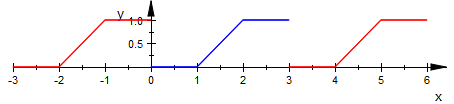
\includegraphics[width=200pt]{images/fourierPeriodischeFortsetzung}\br
Um f ungerade von [0, 3] auf [-3, 3] und anschließend periodisch auf $\R$ fortzusetzen, gilt es eine Punktsymmetrie zum Ursprung herzustellen:\\
f(x) = -f(-x)\\
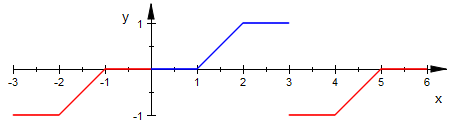
\includegraphics[width=200pt]{images/fourierUngeradeFortsetzung}\br
Um f gerade von [0, 3] auf [-3, 3] und anschließend periodisch auf $\R$ fortzusetzen, gilt es eine Achsensymmetrie zum Y-Achse herzustellen:\\
f(x) = f(-x)\\
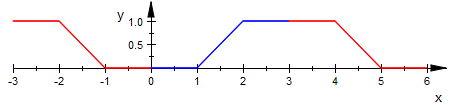
\includegraphics[width=200pt]{images/fourierGeradeFortsetzung}\br
Hier die Ausgangsfunktion f blau eingezeichnet und die jeweilige Fortsetzung in rot.\\
\par	
\endgroup 

3. Regel für $a_k$'s und $b_k$'s erkennen\br

\begingroup
\leftskip2em 
Für symmetrische Funktionen gelten besondere vereinfachende Regeln:\br
Ist f eine gerade Funktion werden alle $b_k$'s = 0.\\
Und ist f eine ungerade Funktion, so werden alle $a_k$'s = 0.\\
\par	
\endgroup 

4. Periodendauer T erkennen\br

\begingroup
\leftskip2em 
Die Periodendauer ist die Länge des Intervalles, ab dem sich die Funktion wiederholt.\\
Für das Beispiel oben ist in der einfachen Fortsetzung T=3 (Intervall:[0, 3]) und für die gerade und ungerade Fortsetzung ist jeweils T=6 (Intervall:[-3, 3]).\\
\par	
\endgroup 

5. $a_k$'s und $b_k$'s berechnen\br

\begingroup
\leftskip2em 
Ist f eine Funktion, die stückweise definiert ist (wie im Beispiel oben), so muss man jedes Stück der Funktion einzeln integrieren und die einzelnen Integrale aufsummieren.\br
Achtung bei Ergebnisse, bei denen ein Bruch für die $a_k$'s oder $b_k$'s entsteht und der Nenner für ein bestimmtes k=$\alpha$ 0 wird. In diesem Fall muss der Wert von $a_\alpha$ / $b_\alpha$ gesondert berechnet werden. (L'Hôspital, $\lim\limits_{k \to \alpha}$, ...) \\
Wichtig:\\
$b_0$ ist immer 0.\\
\par	
\endgroup 
	
6. Reelle Fourierreihe bilden\br

7. [Falls verlangt] Komplexe Fourierreihe bilden\br

\newpage
\section{Rechenbeispiele}

\subsection*{Beispiel 1:}
\bigskip
Sei\\
$
f(x) = \left\{
\begin{array}{l}
0, 0\leq x\leq 1 \\ 
x-1, 1 < x\leq 2 \\
1, 2 < x\leq 3 \\
\end{array}
\right.\\\\
$
Berechnen Sie die reelle und komplexe Fourierentwicklung der Funktion, die entsteht, wenn man f auf $\R$ periodisch fortsetzt.\br


1. Skizze / 2. Periodische Fortsetzung:\\

\begingroup
\leftskip2em 
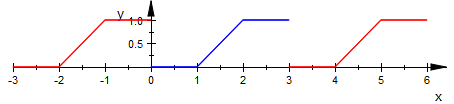
\includegraphics[width=200pt]{images/fourierPeriodischeFortsetzung}\br
\par	
\endgroup 

3. Regel für $a_k$'s und $b_k$'s erkennen:\\

\begingroup
\leftskip2em 
Keine Symmetrie erkennbar. $a_k$'s und $b_k$'s sind nicht einfach 0 zu setzen.\br
\par	
\endgroup 

4. Periodendauer T erkennen:\\

\begingroup
\leftskip2em 
T = 3\br
\par	
\endgroup 

5. $a_k$'s und $b_k$'s berechnen\\

\begingroup
\leftskip2em 
\begin{flalign*}
\hspace{2em}a_k &= \dfrac{2}{T} \cdot \int\limits_{c}^{c+T} f(x) \cdot \cos(\dfrac{2\pi}{T} kx) dx &\\
&=\dfrac{2}{3} \cdot \left( \int\limits_{1}^{2} (x-1) \cdot \cos(\dfrac{2\pi}{3} kx)dx + \int\limits_{2}^{3} 1 \cdot \cos(\dfrac{2\pi}{3} kx)dx \right) &\\
&=\dfrac{9\cos((4\pi k)/3) - 9\cos((2\pi k)/3) + 6\pi k\sin((4\pi k)/3)}{6\pi^2 k^2}&\\
&\hspace*{1em}+ \dfrac{\sin(2\pi k) - \sin((4\pi k)/3)}{\pi k}&\br
\end{flalign*}

\begingroup
\leftskip2em 
$\text{Problem für k=0: Durch 0 darf man nicht teilen.}$\\
$a_0 = 1 $\\
\par	
\endgroup 


\begin{flalign*}
\hspace{2em}b_k &= \dfrac{2}{T} \cdot \int\limits_{c}^{c+T} f(x) \cdot \sin(\dfrac{2\pi}{T} kx)dx&\\
&=\dfrac{2}{3} \cdot \left( \int\limits_{1}^{2} (x-1) \cdot \sin(\dfrac{2\pi}{3} kx)dx + \int\limits_{2}^{3} 1 \cdot \sin(\dfrac{2\pi}{3} kx)dx \right) &\\
&=\dfrac{9\sin((4\pi k)/3) - 9\sin((2\pi k)/3) + 6\pi k(2\sin((2\pi k)/3)^2 - 1)}{6\pi^2 k^2}&\\
& \hspace*{1em}- \dfrac{\cos(2\pi k) - \cos((4\pi k)/3)}{\pi k}&\\
&\text{Problem für k=0: Durch 0 darf man nicht teilen.}&\\
&\text{Aber $b_0$ ist immer 0.} &\\
\end{flalign*}
\par	
\endgroup 

6. Reelle Fourierreihe bilden\\

\begingroup
\leftskip2em 
$ \dfrac{a_0}{2} + \sum\limits_{k=1}^{\infty} (a_k \cdot \cos(\dfrac{2\pi}{T} kx) + b_k \cdot \sin(\dfrac{2\pi}{T} kx)) $\\
$ \dfrac{1}{2} + \sum\limits_{k=1}^{\infty} (a_k \cdot \cos(\dfrac{2\pi}{3} kx) + b_k \cdot \sin(\dfrac{2\pi}{3} kx)) $\br
\par	
\endgroup 

7. Komplexe Fourierreihe bilden\\

\begingroup
\leftskip2em 
$ c_k = \dfrac{1}{2} (a_k - ib_k)$\\
$ \sum\limits_{-\infty}^{\infty} \dfrac{1}{2} (a_k - ib_k) \cdot e^{i\dfrac{2\pi}{3} kx} $\br
\par	
\endgroup 

\newpage
\subsection*{Beispiel 2:}
\bigskip
Sei\\
$
f(x) = \left\{
\begin{array}{l}
1-x^2, 0 \leq x < 1 \\
0, 1 \leq x\leq 2 \\
\end{array}
\right.\\\\
$
Berechnen Sie die reelle und komplexe Fourierentwicklung der Funktion, die entsteht, wenn man f gerade von $[0, 2]$ auf $[-2, 2]$ und anschließend von $[-2, 2]$ auf $\R$ periodisch fortsetzt.\br


1. Skizze / 2. Periodische Fortsetzung:\\

\begingroup
\leftskip2em 
(f in blau, Fortsetzung in rot)\\
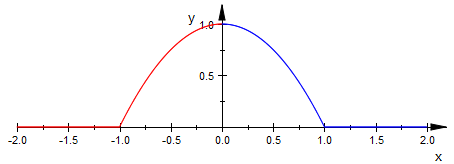
\includegraphics[width=200pt]{images/fourierExample2_1}\\
(Fortsetzung auf $\R$ in grün)\\
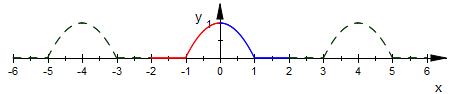
\includegraphics[width=200pt]{images/fourierExample2_2}\br\\
\par	
\endgroup 

3. Regel für $a_k$'s und $b_k$'s erkennen:\\

\begingroup
\leftskip2em 
Die Funktion ist Y-Achsen-Symmetrisch, da sie gerade fortgesetzt wurde. Alle $b_k$'s sind also 0.\br
\par	
\endgroup 

4. Periodendauer T erkennen:\\

\begingroup
\leftskip2em 
T = 4\br
\par	
\endgroup 

5. $a_k$'s und $b_k$'s berechnen\\

\begingroup
\leftskip2em 
\begin{flalign*}
\hspace{2em}a_k &= \dfrac{2}{T} \cdot \int\limits_{c}^{c+T} f(x) \cdot \cos(\dfrac{2\pi}{T} kx) dx &\\
&=\dfrac{1}{2} \cdot \int\limits_{-1}^{1} (1-x^2) \cdot \cos(\dfrac{\pi}{2} kx) dx &\\
&=\dfrac{32\sin(\dfrac{\pi k}{2}) - 16\pi k \cos(\dfrac{\pi k}{2})}{2\pi^3k^3}&\br\\
&\text{Problem für k=0: Durch 0 darf man nicht teilen.}&\\
&a_0 = \dfrac{2}{3} &\\
\end{flalign*}
Alle $b_k$'s sind nach oben genannten Symmetrieeigenschaften 0.\br
\par	
\endgroup

6. Reelle Fourierreihe bilden\\

\begingroup
\leftskip2em 
$ \dfrac{a_0}{2} + \sum\limits_{k=1}^{\infty} (a_k \cdot \cos(\dfrac{2\pi}{T} kx) + b_k \cdot \sin(\dfrac{2\pi}{T} kx)) $\\
$ \dfrac{2}{6} + \sum\limits_{k=1}^{\infty} (a_k \cdot \cos(\dfrac{\pi}{2} kx)) $\br
\par	
\endgroup

7. Komplexe Fourierreihe bilden\\

\begingroup
\leftskip2em 
$ c_k = \dfrac{1}{2} (a_k - ib_k)$\\
$ \sum\limits_{-\infty}^{\infty} \dfrac{1}{2} a_k \cdot e^{i\dfrac{\pi}{2} kx} $\br
\par	
\endgroup

\newpage
\section{Übungsaufgaben}

\subsection*{Aufgabe 1}
Sei\\
$
f(x) = \left\{
\begin{array}{l}
-x^2, x \in [-1,0] \\ 
x^2, x \in [0,1] \\
0, sonst\\
\end{array}
\right.\\\\
$
Berechnen Sie die reelle und komplexe Fourierentwicklung der Funktion, die entsteht, wenn man f vom Intervall $[-1,1]$ auf $\R$ periodisch fortsetzt.\br
	
\subsection*{Aufgabe 2}
Sei\\
$
f(x) = \left\{
\begin{array}{l}
x, 0\leq x\leq 1 \\ 
1-(x-1)^2, 1 < x\leq 2 \\
0, x \geq 2 \\
\end{array}
\right.\\\\
$
Berechnen Sie die reelle und komplexe Fourierentwicklung der Funktion, die entsteht, wenn man f ungerade von $[0,2]$ auf $[-2,2]$ und anschließend auf $\R$ periodisch fortsetzt.\br

\subsection*{Aufgabe 3}
Sei\\
$
f(x) = \left\{
\begin{array}{l}
x, 0\leq x\leq 1 \\ 
1, 1 < x\leq 2 \\
0, 2 < x\leq 3 \\
\end{array}
\right.\\\\
$
Berechnen Sie die reelle und komplexe Fourierentwicklung der Funktion, die entsteht, wenn man f auf $\R$ periodisch fortsetzt.\br

\subsection*{Aufgabe 4}
Sei\br
$
f_1(x) = |cos(x)|\\
f_2(x) = (\sin(x)+\cos(x))^2-1
$\br
Berechnen Sie die reelle und komplexe Fourierentwicklung der Funktionen $f_1(x)$ und $f_2(x)$. Verwenden Sie dabei die kleinstmögliche Periodendauer.\br

\part{Analysis II}

\chapter{Schnittkurven und Parametrisierungen von Körpern und Flächen}

\section{Einleitung}

Für viele der Aufgabentypen wird vorausgesetzt, dass man gut mit geometrischen Körpern im euklidischen dreidimensionalen Raum umgehen kann. Das betrifft vor allem die Abstandsprobleme und die Berechnung von Oberflächen und Volumina von zusammengesetzten Körpern.\\
Deswegen handelt dieses erste Kapitel ausschließlich von der Parametrisierung und Bestimmung von Schnittkurven sich schneidender Körper.

\section{Parametrisierungen: Von kartesischen Gleichungen zu Vektoren und umgekehrt}

\subsection{Grundwissen}

Im folgenden kurz ein Überblick über die wichtigsten Umrechnungen von einfachen Körpern zwischen kartesischen Koordinaten und Vektordarstellung in Polarkoordinaten.

\subsubsection{Kreis}

Kartesische Darstellungsform:

\begingroup
\leftskip2em 
$ (x-x_0)^2+(y-y_0)^2 = r^2 $\\
\par	
\endgroup

Dazugehörige Vektordarstellung in Polarkoordinaten:

\begingroup
\leftskip2em 
$ \left( \begin{matrix}
r\cdot\cos\varphi+x_0\\r\cdot\sin\varphi+y_0\\
\end{matrix} \right), r=0..R, \varphi=0..2\pi $
\par	
\endgroup

\subsubsection{Kugel}

Kartesische Darstellungsform:

\begingroup
\leftskip2em 
$ (x-x_0)^2+(y-y_0)^2+(z-z_0)^2 = r^2 $\\
\par	
\endgroup

Dazugehörige Vektordarstellung in Polarkoordinaten:

\begingroup
\leftskip2em 
$ \left( \begin{matrix}
r\cdot\sin\theta\cdot\cos\varphi+x_0\\r\cdot\sin\theta\cdot\sin\varphi+y_0\\r\cdot\cos\theta+z_0\\
\end{matrix} \right), r=0..R, \varphi=0..2\pi, \theta=0..\pi $
\par	
\endgroup

\subsubsection{Zylinder}

Kartesische Darstellungsform:

\begingroup
\leftskip2em 
Die kartesische Darstellungsform für einen Zylinder, ist die eines Kreises. Nur wird diese nun für den dreidimensionalen Raum interpretiert und nicht für den zweidimensionalen Raum. Das heißt, es gibt jetzt entlang der z-Achse unendlich viele Möglichkeiten den Kreis zu platzieren. So entsteht dann der Zylinder.\\
$ (x-x_0)^2+(y-y_0)^2 = r^2 $\\
\par	
\endgroup

Dazugehörige Vektordarstellung in Polarkoordinaten:

\begingroup
\leftskip2em 
$ \left( \begin{matrix}
r\cdot\cos\varphi+x_0\\r\cdot\sin\varphi+y_0\\z\\
\end{matrix} \right), r=0..R, \varphi=0..2\pi, z=-\infty..\infty $
\par	
\endgroup

\section{Schnittkurven: Einige Spezialfälle}

Auf den folgenden Seiten sind einige Spezialfälle von den Bestimmungen von Schnittkurven gezeigt. Gerechnet und visualisiert wurde hierbei mit dem Programm "MuPAD".

\subsection{Allgemeine Tipps zur Vorgehensweise}

1. Festlegen, welcher der Körper ausschlaggebend für die Höhe, und welcher für die Position auf der X- und Y-Achse ausschlaggebend ist. Wenn leicht entscheidbar ist, welcher Körper für was verantwortlich ist, nimmt einem das einiges an Denkarbeit ab.\\

2. Die Bestimmung einer Höhe lässt sich leicht in kartesischen Koordinaten durchführen, da es für die Höhe die Variable z im Koordinatensystem gibt.\\

3. Man sollte sich je nach Situation entscheiden, ob man das Schnittkurvenproblem in kartesischen oder in Polarkoordinaten angehen möchte. Gerade bei Schnitten von Kugeln oder Zylindern ist es meist hilfreich Polarkoordinaten für die Berechnung zu verwenden, da sich diese leichter in Polarkoordinaten darstellen lassen.\\

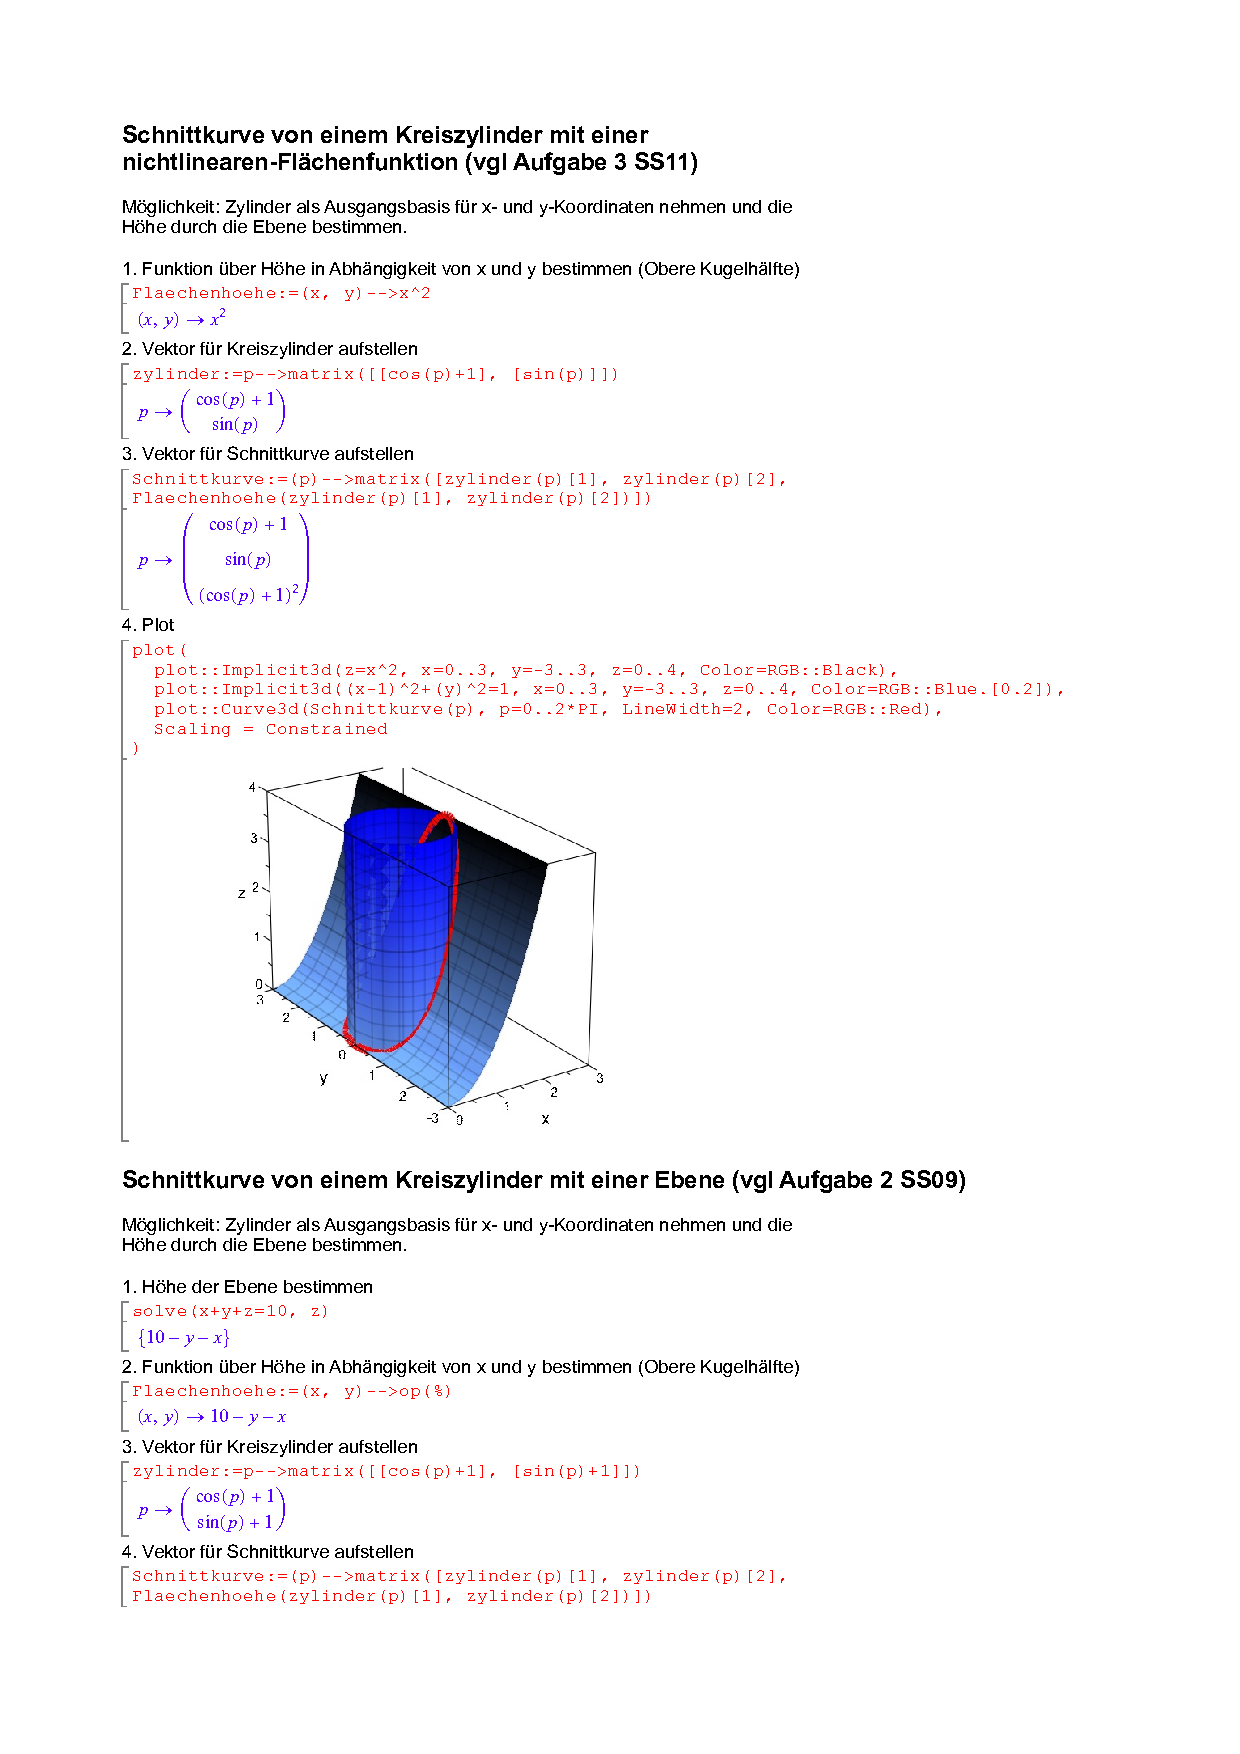
\includepdf[pages=-, pagecommand={\thispagestyle{plain}}]{pdfs/Schnittkurven.pdf}

\chapter{Grundlagen für Klausur und MuPAD}

\section{Grundwissen}
Zur Berechnung von Integralen nach einer Koordinatentransformation benötigt man eine so genannte Jakobimatrix und zur Berechnung von Abständen oder eines Gaußausgleiches benötigt man einen so genannten Gradienten und eine Hessematrix.\\
Was es mit diesen Gebilden auf sich hat wird in diesem Kapitel behandelt.\\

\subsection{Gradient}
Der Gradient einer Funktion $f(\overrightarrow{x}), f:\R^n \rightarrow \R$ ist ein Vektor, der alle partiellen Ableitungen der Funktion $f$ enthält.\\

\textbf{Allgemeine Definition:}\\
$grad(f(\overrightarrow{x})) = \left(\begin{matrix}
\dfrac{\partial}{\partial x_1} \\
\vdots\\
\dfrac{\partial}{\partial x_n} \\
\end{matrix}\right)$\\

\textbf{Beispiel:}\\

Sei $f(x, y) = x^2y^2 $.\\

Dann ist der Gradient von $f$:\\
$grad(f(x, y)) = \left(\begin{matrix}
2xy^2 \\
2x^2y \\
\end{matrix}\right)$.\\

\subsection{Jakobimatrix}
Die Jakobimatrix die mehrdimensionale Verallgemeinerung des Gradienten für Funktionen wie $f(\overrightarrow{x}), f:\R^n \rightarrow \R^m$ und ist eine $m \times n$-Matrix, die alle partiellen Ableitungen der Funktion $f$ enthält.\\

\textbf{Allgemeine Definition:}\\
$J_f(\overrightarrow{x}) = \left(\begin{matrix}
\dfrac{\partial f_1}{\partial x_1} & \dfrac{\partial f_1}{\partial x_2} &\cdots & \dfrac{\partial f_1}{\partial x_n} \\
\dfrac{\partial f_2}{\partial x_1} & \dfrac{\partial f_2}{\partial x_2} &\cdots & \dfrac{\partial f_2}{\partial x_n} \\
\vdots & \vdots & \ddots &\vdots\\
\dfrac{\partial f_m}{\partial x_1} & \dfrac{\partial f_m}{\partial x_2} & \cdots & \dfrac{\partial f_m}{\partial x_n} \\
\end{matrix}\right)$\\

\textbf{Beispiel:}\\
Sei $f(x, y) = \left(\begin{matrix}
2xy^2 \\
2x^2y \\
\end{matrix}\right)$.\\

Dann ist die Jakobimatrix von $f$:\\
$J_f(x, y) = \left(\begin{matrix}
2y^2 & 4xy \\
4xy & 2x^2 \\
\end{matrix}\right)$.\\

\subsection{Hessematrix}
Die Hessematrix einer Funktion $f(\overrightarrow{x}), f:\R^n \rightarrow \R$ ist eine Matrix, die alle partiellen zweiten Ableitungen der Funktion $f$ enthält.\\

\textbf{Zusammenhang mit Gradient und Jakobimatrix:}\\
Es gilt folgende Gleichung, die den Zusammenhang zwischen der Hessematrix, der Jakobimatrix und dem Gradienten beschreibt:\\

$ H_f(\overrightarrow{x}) = J_f(grad(f(\overrightarrow{x})) $\\

Also: Die Jakobimatrix des Gradienten der Funktion f, ist das Gleiche wie die Hessematrix der Funktion.\\

\textbf{Allgemeine Definition:}\\
$H_f(\overrightarrow{x}) = \left(\begin{matrix}
\dfrac{\partial^2 f}{\partial x_1 \partial x_1} & \dfrac{\partial^2 f}{\partial x_1 \partial x_2} &\cdots & \dfrac{\partial^2 f}{\partial x_1 \partial x_n} \\
\dfrac{\partial^2 f}{\partial x_2 \partial x_1} & \dfrac{\partial^2 f}{\partial x_2 \partial x_2} &\cdots & \dfrac{\partial^2 f}{\partial x_2 \partial x_n} \\
\vdots & \vdots & \ddots &\vdots\\
\dfrac{\partial^2 f}{\partial x_n \partial x_1} & \dfrac{\partial^2 f}{\partial x_n\partial x_2} & \cdots & \dfrac{\partial^2 f}{\partial x_n \partial x_n} \\
\end{matrix}\right)$\\

\textbf{Beispiel:}\\

Sei $f(x, y) = x^2y^2 $.\\

Dann ist die Hessematrix von $f$:\\
$H_f(x, y) = \left(\begin{matrix}
2y^2 & 4xy \\
4xy & 2x^2 \\
\end{matrix}\right)$.\\

\newpage
\section{Übungen}

\textbf{Aufgabe 1:}\\
Sei $f(x, y) = 3x^4y^5+5x^2 $.\\
Berechnen Sie den Gradienten von $f$.\\

\textbf{Aufgabe 2:}\\
Sei $f(x, y) = xy^2sin(x)e^y $.\\
Berechnen Sie den Gradienten von $f$.\\

\textbf{Aufgabe 3:}\\
Sei $f(x, y, z) = \left(\begin{matrix}
5x^2yz^3\\
4x^2+y+z \\
xz\\
\end{matrix}\right)$.\\
Berechnen Sie die Jakobimatrix von $f$.\\

\textbf{Aufgabe 4:}\\
Sei $f(x, y) = \left(\begin{matrix}
6x^3y^4\\
4x+5e^{y^2} \\
\sin(5x^2)\\
\end{matrix}\right)$.\\
Berechnen Sie die Jakobimatrix von $f$.\\

\textbf{Aufgabe 5:}\\
Sei $f(x) = 3x^4+5x^2 $.\\
Berechnen Sie die Hessematrix von $f$.\\

\textbf{Aufgabe 6:}\\
Sei $f(x, y, z) = x^3y^2+5x^2z^3+5yz $.\\
Berechnen Sie die Hessematrix von $f$.\\

\newpage
\section{MuPAD - Befehlsübersicht}

\begin{tabular}{|p{5cm}|p{10cm}|}
\hline 
linalg::crossProduct(V1, V2) & Berechnet das Kreuzprodukt der Vektoren V1 und V2 \\ 
\hline 
linalg::scalarProduct(V1, V2) & Berechnet das Skalarprodukt der Vektoren V1 und V2 \\ 
\hline 
linalg::det(QM) & Berechnet die Determinante der quadratischen Matrix QM \\ 
\hline 
linalg::grad(f(p), [p]) & Berechnet von einer Funktion f(p) den Gradienten bezüglich der Parameter p. \\ 
\hline 
linalg::jacobian(f(p), [p]) & Berechnet von einer Funktion f(p) die Jakobimatrix bezüglich der Parameter p. \\ 
\hline 
linalg::hessian(f(p), [p]) & Berechnet von einer Funktion f(p) die Hessematrix bezüglich der Parameter p. \\ 
\hline 
linalg::divergence(V(p), [p]) & Berechnet die Divergenz des Vektorfeldes V(p) bezüglich der Parameter p. \\
\hline 
linalg::matlinsolve(A, B) & Löst die Gleichung AX = B und gibt die Lösung zurück. \\
\hline 
solve({A}, {p}) & Löst den Ausdruck A nach den Parametern p auf. \\
\hline 
norm(V) & Berechnet von einem Vektor V den Betrag. \\ 
\hline 
fp::unapply(T, p) & Macht aus Ausdruck T eine Funktion mit den Param. p. \\
\hline 
\_plus(A(k)\$k=1..n) & Berechnet die Summe aller A(k) für k=1..n \\
\hline 
op(A) & Entfernt die äußersten Klammern um den Ausdruck A \\
\hline 
\end{tabular}\\ 

\section{Mehrdimensionales Newtonverfahren}

Das mehrdimensionale Newtonverfahren dient dem Lösen von nicht linearen Gleichungssystemen.\\
Es ist wie auch das eindimensionale Newtonverfahren rekursiv definiert.\\
Definiert werden muss ein Startvektor X.\\

X:=matrix([x1, ..., xn]);\\

Anschließend löst man das Gleichungssystem Ad = B, mit A=Hessematrix der Ausgangsfunktion und B=negativer Gradient der Ausgangsfunktion.\\
Die Lösung d dieses Gleichungssystems gibt den Fehler des Startwertes an und man korrigiert den Startwert um diesen Fehler.\\
Das ganze führt man N mal aus. In der Praxis lang meist je nach Güte des Startwertes schon ein N<=10 um ein gutes Ergebnis zu erzielen.\\
Um zu überprüfen, ob das Newtonverfahren konvergiert sollte man den Betrag des Fehlervektors d ausgeben. Ist der Betrag 0, ist das Newtonverfahren konvergent.\\

for k from 1 to N do\\
\hspace*{2em}d:=float(linalg::matlinsolve(JgradF(X[k]\$k=1..n),-gradF(X[k]\$k=1..n))):\\
\hspace*{2em}X:=X+d:\\
\hspace*{2em}print(norm(d));\\
end\_for;\\

\newpage
\section{Übungen}

\textbf{Aufgabe 1:}\\
Kontrollieren Sie alle Rechnungen von Übung 15.2. mit MuPAD.\\

\textbf{Aufgabe 2:}\\
Seien $\overrightarrow{x} = \left(\begin{matrix}
2x\\
4y^2 \\
z\\
\end{matrix}\right)$ und $\overrightarrow{y} = \left(\begin{matrix}
x^2\\
y \\
25z^3\\
\end{matrix}\right)$ zwei Vektoren.\\

a) Berechnen Sie das Kreuzprodukt der Vektoren mit MuPAD.\\
b) Berechnen Sie das Skalarprodukt der Vektoren mit MuPAD.\\

\textbf{Aufgabe 3:}\\

Berechnen Sie die Determinante der Jakobimatrix der Transformationsmatrix von:\\

a)Transformationsmatrix  von kartesischen Koordinaten zu Polarkoordinaten\\
\hspace*{2em}$\left(\begin{matrix}
r\cos(\varphi)\\
r\sin(\varphi)\\
\end{matrix}\right)$.\br

b)Transformationsmatrix von kartesischen Koordinaten zu Kugelkoordinaten\\
\hspace*{2em}$\left(\begin{matrix}
r\sin(\theta)\cos(\varphi)\\
r\sin(\theta)\sin(\varphi)\\
r\cos(\theta)\\
\end{matrix}\right)$.\br

\textbf{Aufgabe 4:}\\

Lösen Sie folgendes Gleichungssystem mit dem solve()-Befehl von MuPAD:\\
$\left(\begin{matrix}
688a + 504b + 144c - 5462.56775\\
504a + 432b + 112c - 4265.21985\\
144a + 112b + 32c - 1183.416763\\
\end{matrix}\right) = \overrightarrow{0}$\br

\textbf{Aufgabe 5:}\\
Sei $f(x1, y1, x2, y2, l1, l2) = (x1-x2)^2+(y1-y2)^2+l2((x2-3)^2+y2^2-1)+l1((x1-2)^2+3(y -3)^2-1)$ eine Funktion.\\

a) Berechnen Sie den Gradienten der Funktion $f$.\\
b) Berechnen Sie die Hessematrix der Funktion $f$.\\
c) Führen Sie das Newtonverfahren für die Funktion f durch mit dem Startvektor\\
\hspace*{2em}$\overrightarrow{X} = \left(\begin{matrix}
1\\
1\\
0\\
-2.5\\
17\\
17\\
\end{matrix}\right)$

\chapter{Abstandsprobleme (Normal)}

\section{Einleitung}
Bei dem Aufgabentyp ''Abstandsprobleme'' geht es wie der Name schon sagt darum den Abstand zwischen zwei geometrischen Figuren zu berechnen.\\
Beziehungsweise geht es darum, den geringsten Abstand zwischen den Figuren zu ermitteln.\\
In einer Klausuraufgabe sind meist zwei Figuren in unterschiedlichen Darstellungsformen gegeben. Das heißt für das erfolgreiche Bearbeiten einer solchen Aufgabe ist es wichtig, dass man sicher im parametrisieren von Körpern/Figuren in verschiedenen Darstellungsformen ist.\\
Diese Art der Herangehensweise eignet sich für Figuren, die in Vektordarstellung leicht parametrisiert werden können. Für schwere implizite Funktionen ist die Methode nach Lagrange 

Eine typische Klausuraufgabe könnte folgendermaßen aussehen:\\

\textbf{Aufgabe} (1500) [6 Punkte] Berechnen Sie den Abstand der Kurve\br
$ \omega(t)=\left(\begin{matrix}
4\cos(t)\\ 
4\sin(t)\\ 
t^2(2\pi-t)^2
\end{matrix}\right), t\in[0, 2\pi] $\br
von der Schittkurve der Flächen\\

$ (x-8)^2+y^2=4 $\\
$ x+y+z = 60 $.\\

Diese Aufgabe wird in diesem Kapitel als Rechenbeispiel dann gelöst werden.\\

\section{Ablaufplan}
Die Berechnung eines Abstandes läuft immer nach dem gleichen Schema ab:\\

1. Die aus der Aufgabenstellung gegebenen n-dimensionalen Figuren (hier $g$ und $f$) in Vektordarstellung bringen:\\

\begingroup
\leftskip2em 
$ f(\overrightarrow{x_1})=\left(\begin{matrix}
x_1\\
\vdots\\
x_n
\end{matrix}\right) $ und $ g(\overrightarrow{y_1})=\left(\begin{matrix}
y_1\\
\vdots\\
y_n
\end{matrix}\right) $\\
\par	
\endgroup

2. Die Zielfunktion aufstellen.\\

\begingroup
\leftskip2em 
$ F(\overrightarrow{x}) = ||f(\overrightarrow{x_1})-g(\overrightarrow{y_1})||^2 $\\
\par	
\endgroup

3. Gradient und Hessematrix der Zielfunktion berechnen.\\

\begingroup
\leftskip2em 
$ gradF(\overrightarrow{x}) = grad(F) $\\
$ HessF(\overrightarrow{x}) = JgradF(\overrightarrow{x}) = J_{gradF(F)} $\\
\par	
\endgroup

4. Startwert bestimmen.\\

\begingroup
\leftskip2em 
Der Startwert wird für die Klausur nicht rechnerisch bestimmt, sondern anhand einer gegebenen Skizze bzw. anhand eines MuPAD-Plottes abgeschätzt. Es gibt für den Startwert kein ''richtig'' oder ''falsch'', sondern nur ''okay'' oder ''total daneben''. Nur ein Startwert der komplett von dem reellen Wert abweicht liefert hier keine Klausurpunkte.\\
Von der Güte des Startwertes hängt es ab, ob und wie schnell das Newtonverfahren am Ende konvergiert.\\
\par	
\endgroup

5. Newtonverfahren durchführen.\\

\begingroup
\leftskip2em 
Das Newtonverfahren wird in der Klausur mit MuPAD durchgeführt. Man programmiert dafür eine Schleife, die folgendermaßen aussieht:\\

for k from 1 to N do\\
\hspace*{2em}d:=float(linalg::matlinsolve(JgradF(X[k]\$k=1..n),-gradF(X[k]\$k=1..n))):\\
\hspace*{2em}X:=X+d:\\
\hspace*{2em}print(norm(d));\\
end\_for;\\

N ist hierbei die Anzahl der Iterationen die ihr durchführen wollt. Mit 10 Schritten seid ihr aber auf der sicheren Seite. Meistens braucht das Newtonverfahren wenige Schritte zum Konvergieren. Es kommt natürlich auch ein wenig auf den Startwert an.\\
n ist die Anzahl der Parameter der Funktion.\\

\par	
\endgroup

6. Ergebnisvektor anzeigen.\\

\begingroup
\leftskip2em 
Den Ergebnisvektor mit MuPAD ausgeben um ihn dokumentieren zu können.\\
\par	
\endgroup

7. Ergebnis überprüfen.\\

\begingroup
\leftskip2em 
Mit MuPAD einen Plot durchführen. Die beiden Punkte auf den Figuren berechnen, die durch den Ergebnisvektor entstanden sind. (Hierzu die Koordinaten aus dem Ergebnisvektor in die Funktionen einsetzen). Anschließend zwischen den Punkten eine Linie ziehen. Eignet sich als Plausibilitätskontrolle. Sollte der Plot nicht stimmen, sollte dies in der Klausur dokumentiert werden. (Rettet eventuell den einen oder anderen Punkt.)\\
\par	
\endgroup

8. Abstand berechnen.\\

\begingroup
\leftskip2em 
Die Koordinaten aus dem Ergebnisvektor in die Ausgangsfunktionen einsetzen, die Differenz zwischen den Funktionen berechnen und von dem Differenzvektor den Betrag bilden.\\
\par	
\endgroup

\newpage
\section{Zielfunktion}

Die Zielfunktion bis nach der Methode der kleinsten quadratischen Fehler durchgeführt.\\
Man subtrahiert hierbei den einen Vektor komponentenweise von dem anderen und summiert anschließend über die Quadrate der einzelnen Komponenten.\\

Beispiel:\\

\begingroup
\leftskip2em 
Seien $ f(x_1, y_1)=\left(\begin{matrix}
x_1\\
y_1
\end{matrix}\right) $ und $ g(x_2, y_2)=\left(\begin{matrix}
x_2\\
y_2
\end{matrix}\right) $.\br

Dann stellen wir die Zielfunktion folgendermaßen auf:\\
$ F(x_1, y_1, x_2, y_2) = (x_1-x_2)^2+(y_1-y_2)^2 $\\

Das entspricht dem Quadrat des Betrages des Differenzvektors:\\
$ F(\overrightarrow{x}) = ||f(\overrightarrow{x_1})-g(\overrightarrow{y_1})||^2 $\\
\par	
\endgroup

Wichtig für das Aufstellen der Zielfunktion ist, dass beide Figuren aus der Aufgabenstellung in eine vektorielle Darstellungsform gebracht werden und das beide Vektoren die gleiche Anzahl an Dimensionen haben. Die Anzahl der Parameter ist hierbei irrelevant.\\

Beispiel:\\

\begingroup
\leftskip2em 
Seien $ f(x, y)=\left(\begin{matrix}
x\\
y
\end{matrix}\right) $ und $ g(p)=\left(\begin{matrix}
p\\
p^2
\end{matrix}\right) $.\br

Dann stellen wir die Zielfunktion folgendermaßen auf:\\
$ F(x_1, y_1, p) = (x-p)^2+(y-p^2)^2 $
\par	
\endgroup

\newpage
\section{Rechenbeispiel}

\textbf{Aufgabe} (1500) [6 Punkte] Berechnen Sie den Abstand der Kurve\br
$ \omega(t)=\left(\begin{matrix}
4\cos(t)\\ 
4\sin(t)\\ 
t^2(2\pi-t)^2
\end{matrix}\right), t\in[0, 2\pi] $\br
von der Schittkurve der Flächen\\

$ (x-8)^2+y^2=4 $\\
$ x+y+z = 60 $.\\

\subsection{MuPAD Lösung}

1. Beide gegebenen Kurven parametrisieren und in Vektordarstellung überführen.\\
(Der zweite Vektor ist die Schnittkurve zwischen einem Zylinder und einer Fläche. Dieser Spezialfall wird im Kapitel ''Schnittkurven und Parametrisierungen von Körpern'' näher erläutert)\\

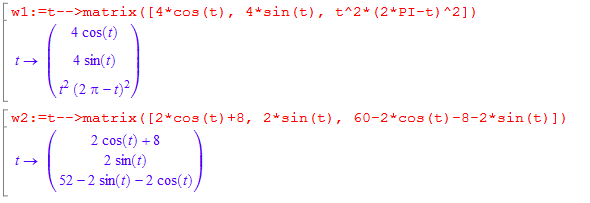
\includegraphics[scale=2.2]{images/abstandsproblem/param.png}

2. Zielfunktion aufstellen.\\

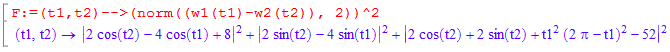
\includegraphics[scale=2.2]{images/abstandsproblem/zielfkt.png}

3. Gradient und Hessematrix berechnen.\\

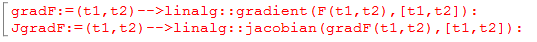
\includegraphics[scale=2.2]{images/abstandsproblem/grad.png}

4. Startwert bestimmen.\\

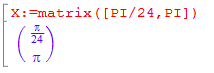
\includegraphics[scale=2.2]{images/abstandsproblem/start.png}

5. Newtonverfahren durchführen.\\

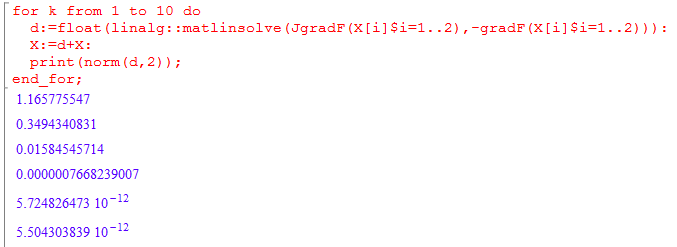
\includegraphics[scale=2.2]{images/abstandsproblem/newton.png}

6. Ergebnis anzeigen.\\

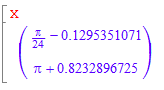
\includegraphics[scale=2.2]{images/abstandsproblem/result.png}

7. Ergebnis überprüfen.\\

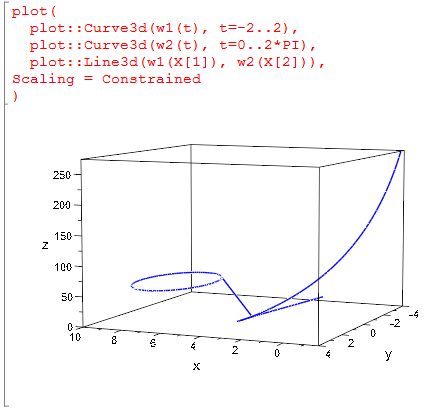
\includegraphics[scale=2.2]{images/abstandsproblem/plot.png}

8. Abstand berechnen.\\

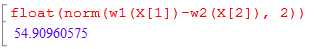
\includegraphics[scale=2.2]{images/abstandsproblem/abstand.png}

\subsection{Klausurdokumentation}

Die am häufigsten gestellte Frage in ANA II ist: Wie muss ich das ganze dann in der Klausur dokumentieren?\\
Die besten MuPAD-Rechnungen sind nutzlos, wenn sie nicht auch zu Papier gebracht werden können.\\
Aus den folgenden Seiten mal ein Beispiel von mir, wie so eine Klausuraufgabe dann dokumentiert aussehen kann:\\

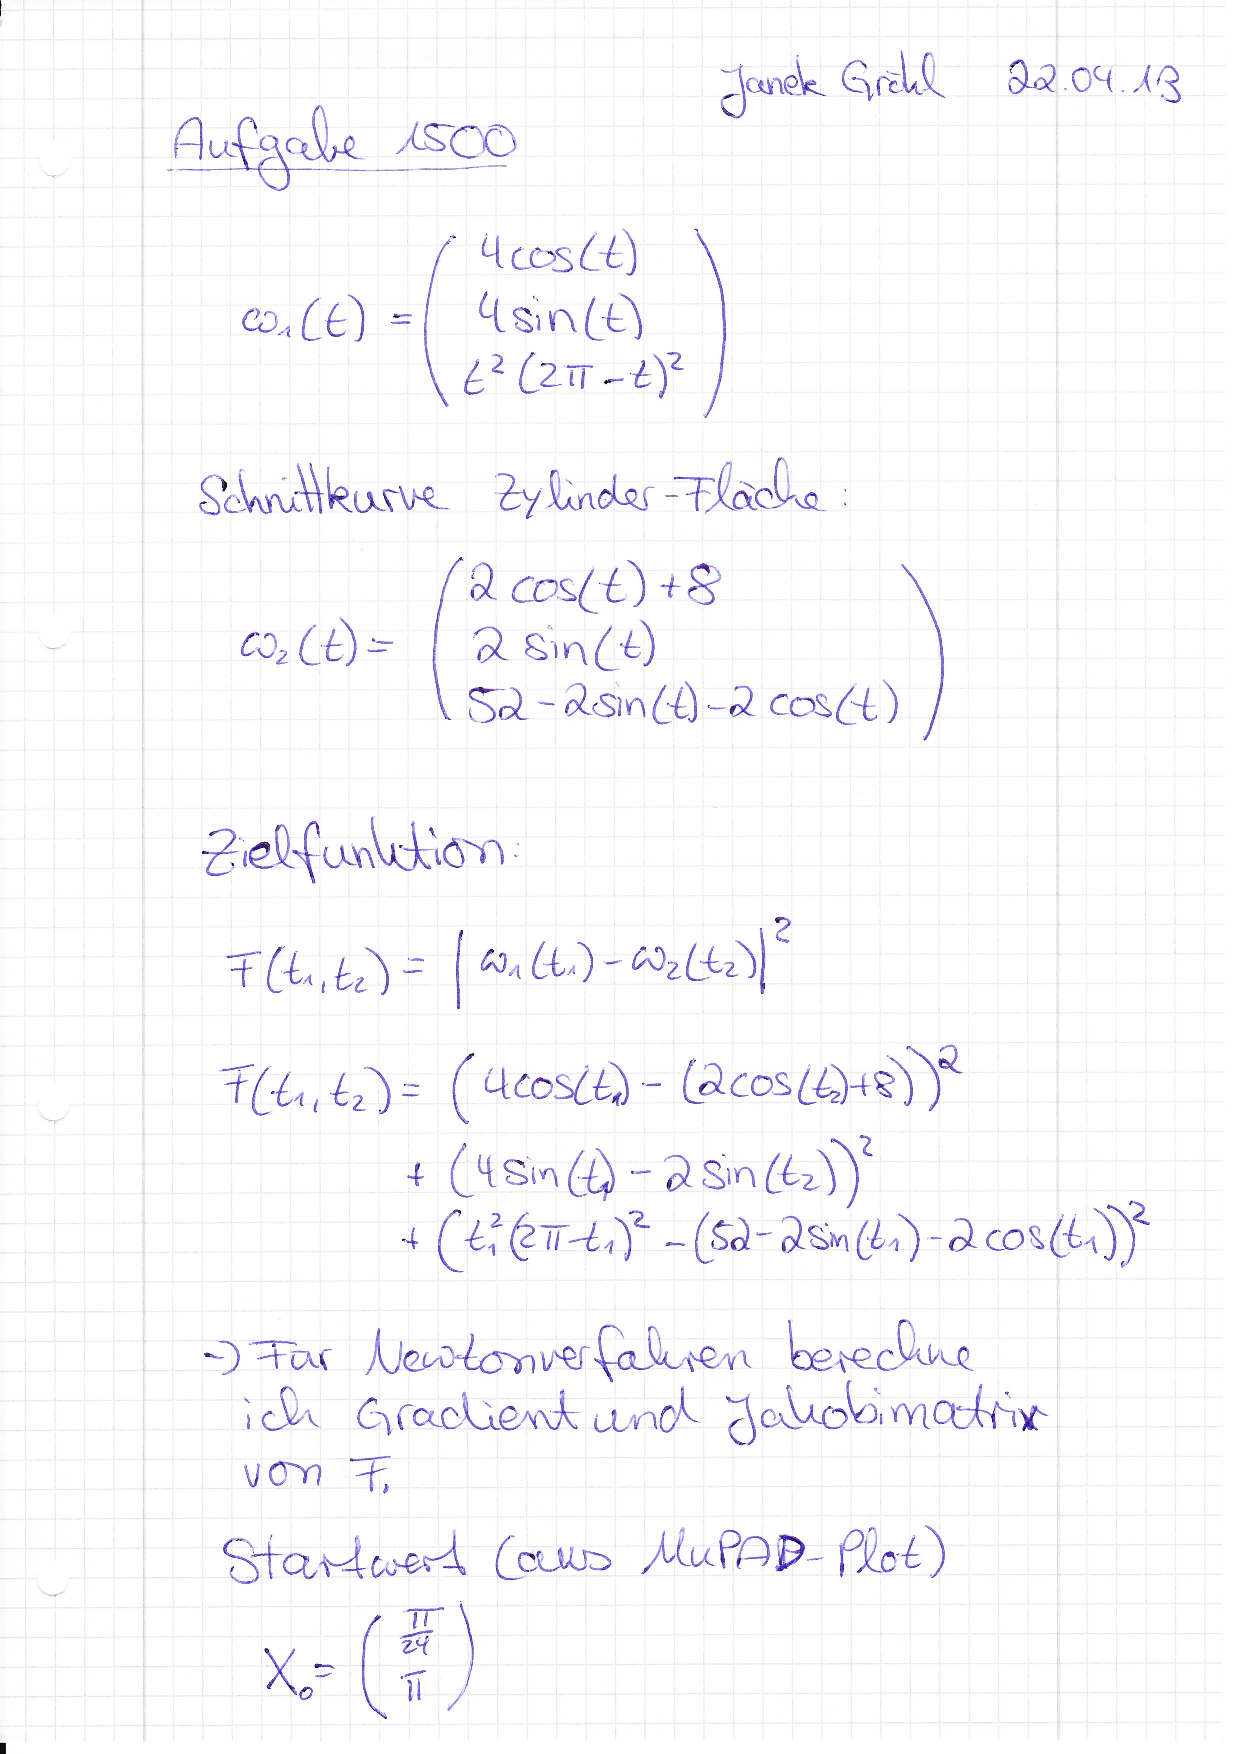
\includepdf[pages=-, pagecommand={\thispagestyle{plain}}]{pdfs/Abstandsprobleme_Normal_Beispiel.pdf}

\section{Übungsaufgaben}

\textbf{Aufgabe 1} (938) [6 Punkte]\\

\begingroup
\leftskip2em 

Berechnen Sie den Abstand der Kurve\br
$ \omega(t)=\left(\begin{matrix}
t\\ 
\sin(t)\\ 
0
\end{matrix}\right), t\in\R $\br
von der Fläche\\
$ z=2+(x-1)^2+y^2, x, y \in \R $\\

\par	
\endgroup

\textbf{Aufgabe 2} (1261) [6 Punkte]\\

\begingroup
\leftskip2em 

Berechnen Sie den Abstand der Kurven\br
$ \omega(t)=\left(\begin{matrix}
5+\cos(t)\\ 
2\sin(t)\\ 
6+\sin(t)+\cos(t)
\end{matrix}\right), t\in\R $\br
und\\
$ x^2+y^2=1, z=2 $\\
voneinander. Verwenden Sie das Newton-Verfahren.\\

\par	
\endgroup

\textbf{Aufgabe 3} (1008) [8 Punkte]\\

\begingroup
\leftskip2em 

Berechnen Sie den Abstand der Flächen\\
$ f(x, y) = (x-y+1)^2+2y^4+10$\\\
und\\
$ g(x, y) = -(x+y-12)^2-y^4-20$\\
voneinander. Verwenden Sie das Newton-Verfahren.\\

\par	
\endgroup

\textbf{Aufgabe 4} [6 Punkte]\\

\begingroup
\leftskip2em 

Berechnen Sie den Abstand der Kurven\\
$ y=3+x^2+\dfrac{1}{x}$\\\
und\\
$ x^2-y^2=1$\\
für $x>0$ voneinander. Verwenden Sie das Newton-Verfahren.\\

\par	
\endgroup

\chapter{Abstandsprobleme (Lagrange-Funktion)}

\section{Einleitung}
Die im vorherigen Kapitel besprochene Methode zur Berechnung von Minima/Maxima funktioniert nur, wenn man die entsprechenden zu minimierenden Funktionen in Vektordarstellung bringen kann. Ansonsten ist es nicht möglich eine geeignete Zielfunktion nach der vorgestellten Methode zu finden.\\
Auch kann es manchmal umständlich sein implizite Ausdrücke nach einer Variablen aufzulösen, um einen Vektor aufstellen zu können.\\

Ein Beispiel hierzu:\\

Berechnen Sie den Abstand der Kurven

\begingroup
\leftskip2em 
$ y=3+x^2+1/x $ und\\
$ x^2-y^2=1 $
\par	
\endgroup

für $x>0$ voneinander. (Übungsaufgabe 4 des vorherigen Kapitels).\\

Für die erste Kurve ist es noch sehr leicht einen Vektor zu finden mit\\ 
$\left(\begin{matrix}
x\\ 3+x^2+1/x\\
\end{matrix}\right)$.\\ 

Doch für die zweite Kurve wird das schon ein wenig komplizierter mit\\
$\left(\begin{matrix}
x\\ \pm\sqrt{x^2-1}\\
\end{matrix}\right)$.

Die Frage ist bei der zweiten Gleichung nämlich: welches Vorzeichen muss jetzt für die Wurzel gewählt werden?\\
Das ist dann noch ein harmloseres Beispiel, aber man kann sich leicht vorstellen, dass es Terme gibt, die sich überhaupt nicht leicht nach einem Parameter auflösen lassen.\\
Um sich solche Probleme vereinfachen zu können gibt es die Lagrange-Funktion. Über die Lagrange-Funktion kann man Nebenbedingungen in das Minimierungs-/Maximierungsproblem mit einbauen und stellt einfach eine andere Art von Zielfunktion dar.\\

\section{Ablaufplan}

Am eigentlichen Ablaufplan des vorherigen Kapitels ändert sich nichts. Lediglich die ersten beiden Schritte zum Erstellen der Zielfunktion müssen an die Lagrangefunktion angepasst werden:\\

1. Die gegebenen Kurven in folgende implizite Form überführen:

\begingroup
\leftskip2em 
$f(\overrightarrow{x})=0$\\
Hierzu einfach alle Terme auf eine Seite des Gleichheitszeichens bringen.\\
Diese impliziten Gleichungen stellen dann im 2. Schritt die Nebenbedingungen für die Zielfunktion dar.\\
\par	
\endgroup

2. Die Zielfunktion erstellen:

\begingroup
\leftskip2em 
Die Lagrangefunktion hat folgende Struktur:\\
$ L(x_1, y_1, ..., x_n, y_n, l_1, ..., l_m) = (x_1-y_1)^2+...+(x_n-y_n)^2+l_1\cdot(NBDG_1)+...+l_m\cdot(NBDG_m)$\\
Die entsprechenden Terme für die Nebenbedingungen ergeben sich dann aus den Gleichungen aus Schritt 1.\\
Die Parameter $l_1, ..., l_m$ heißen Lagrangeparameter.
\par	
\endgroup

\section{Lagrange-Funktion}

Wie eben schon kennengelernt hat die Lagrangefunktion folgendes Aussehen:\\
$ L(x_1, y_1, ..., x_n, y_n, l_1, ..., l_m) = (x_1-y_1)^2+...+(x_n-y_n)^2+l_1\cdot(NBDG_1)+...+l_m\cdot(NBDG_m)$\\

Beim Einfügen der Nebenbedingungen ist auf die Wahl der richtigen Parameter für die Terme zu achten. Für eine der Figuren sind die Parameter $x_1, ..., x_n$ und für die andere Figur die Parameter $y_1, ..., y_n$ reserviert. Eine Figur könnte sich theoretisch aus mehreren Nebenbedingungen zusammensetzen. Ist dies der Fall muss darauf geachtet werden, dass alle Nebenbedingungen einer Figur die gleichen Parameter haben. (Beispiel zur Verdeutlichung in den Rechenbeispielen).\\
Gleiches gilt dann umgekehrt für verschiedene Figuren: Verschiedene Figuren dürfen nicht gleiche Parameter haben.\\

\subsection{Startwert}

Bei der Wahl für den Startvektor kann man aus Skizzen keine Schätzungen für die Lagrangeparameter angeben. Man darf diese Parameter \textbf{niemals} $0$ setzen, da die Nebenbedingungen ansonsten ja nicht vorhanden sind. $17$ oder $\sqrt{17}$ sind gute Startwerte : D\\
Die Parameter $x_1, y_1, ..., x_n, y_n$ können wieder wie zuvor aus der Skizze entnommen werden.

\section{Rechenbeispiele}

\subsection{Aufgabe 1 (einfach)}

\textbf{Aufgabe} [6 Punkte] Berechnen Sie den Abstand der Kurven\br
$(x-3)^2+8(y-3)^2=4$\br
und\\
$8(x-3)^2+y^2=4$.\\

\subsection{MuPAD Lösung}

1. Beide gegebenen Kurven in die form f(x, y)=0 überführen und definieren.\\

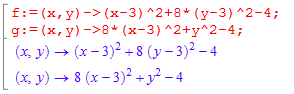
\includegraphics[scale=2.2]{images/abstandsproblem2/param.png}

2. Zielfunktion mit Lagrangeparametern und Nebenbedingungen aufstellen.\\

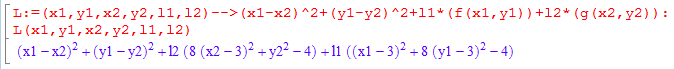
\includegraphics[scale=2.2]{images/abstandsproblem2/zielfkt.png}

3. Gradient und Hessematrix berechnen.\\

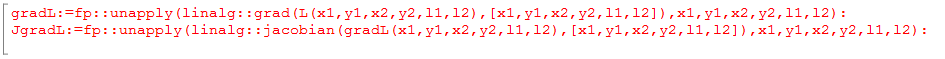
\includegraphics[width=15cm]{images/abstandsproblem2/grad.png}

4. Startwert bestimmen.\\

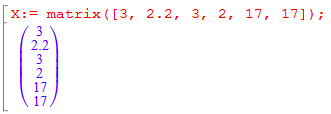
\includegraphics[scale=2.2]{images/abstandsproblem2/start.png}

5. Newtonverfahren durchführen.\\

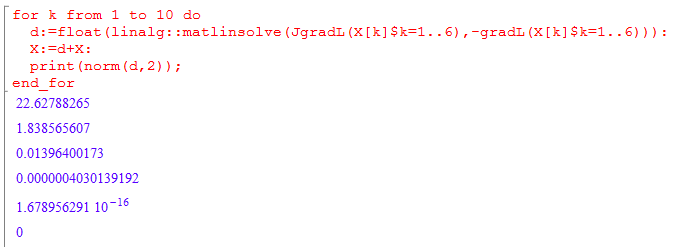
\includegraphics[scale=2.2]{images/abstandsproblem2/newton.png}

6. Ergebnis anzeigen.\\

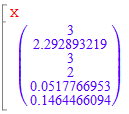
\includegraphics[scale=2.2]{images/abstandsproblem2/result.png}

7. Ergebnis überprüfen.\\

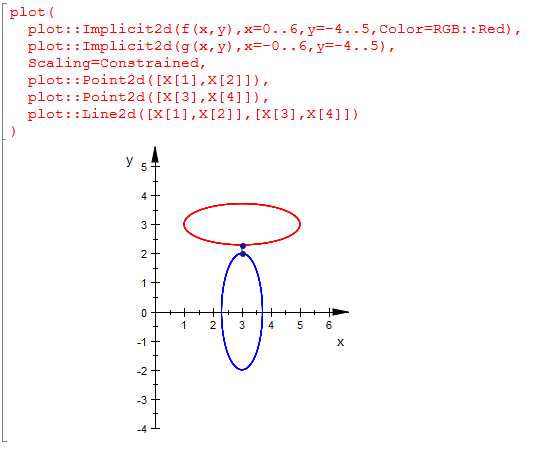
\includegraphics[scale=2.2]{images/abstandsproblem2/plot.png}

8. Abstand berechnen.\\

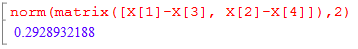
\includegraphics[scale=2.2]{images/abstandsproblem2/abstand.png}

\subsection{Aufgabe 2 (komplexer)}

\textbf{Aufgabe} [6 Punkte] Berechnen Sie den Abstand der Schnittkurven von\br
$(x-2)^2+3(y-1)^2+(z-1)^2=1$\\ mit\\
$f(x, y)=x+y-1$\gbr
und\gbr
$(x-3)^2+5(y+1)^2+5(z+1)^2=4$.\\ mit\\
$f(x,y)=(x-2)^2-y-4$\\

\subsection{MuPAD Lösung}

1. Beide gegebenen Kurven in die form f(x, y)=0 überführen und definieren.\\

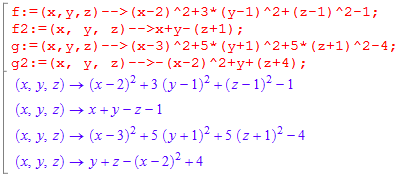
\includegraphics[scale=2.2]{images/abstandsproblem3/param.png}

2. Zielfunktion mit Lagrangeparametern und Nebenbedingungen aufstellen.\\

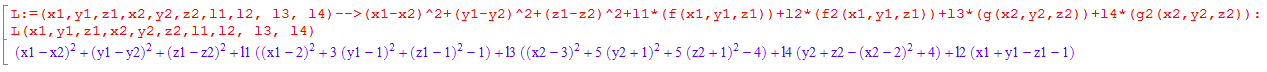
\includegraphics[width=15cm]{images/abstandsproblem3/zielfkt.png}

3. Gradient und Hessematrix berechnen.\\

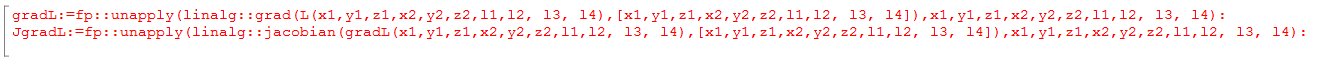
\includegraphics[width=15cm]{images/abstandsproblem3/grad.png}

4. Startwert bestimmen.\\

\includegraphics[scale=2.2]{images/abstandsproblem3/start.png}
\newpage
5. Newtonverfahren durchführen.\\

\includegraphics[scale=2.2]{images/abstandsproblem3/newton.png}

6. Ergebnis anzeigen.\\

\includegraphics[scale=2.2]{images/abstandsproblem3/result.png}

7. Ergebnis überprüfen.\\

\includegraphics[scale=2.2]{images/abstandsproblem3/plot.png}

8. Abstand berechnen.\\

\includegraphics[scale=2.2]{images/abstandsproblem3/abstand.png}

\section{Übungsaufgaben}

\subsection{Aufgabe 1}

[6 Punkte] Bestimmen Sie den Abstand der Fläche\\
$ f(x, y) = x^2 + y^2/4 + 2 $\\
von dem Punkt $\left(\begin{matrix}
0.5\\0\\3\\
\end{matrix}\right) $.\\

\subsection{Aufgabe 2}

[6 Punkte] Berechnen Sie den Abstand der Kurven\\
$(x - 2)^2 + 3(y - 1)^2 = 4$\\
und\\
$2(x + 5)^2 + (y + 2)^2 = 16$\\
voneinander.\\

\subsection{Aufgabe 3}
(1326) [6 Punkte]\\
Eine Kugel um $\left( \begin{matrix}
3\\2\\1\\
\end{matrix} \right) $ vom Radius $r=2$ werde mit der Ebene $2x-4y+z=3$ geschnitten. Welchen Abstand hat die Schnittkurve beider Flächen von dem Punkt $\left( \begin{matrix}
5\\-1\\2\\
\end{matrix} \right) $?\\

\subsection{Aufgabe 4}
[6 Punkte] Berechnen Sie den Abstand der Schnittkurven von\\
$(x-3)^2+(y-1)^2+(z-1)^2/2=1$\\ mit\\
$f(x, y)=(x-2)^2+y^2-1$\gbr
und\gbr
$(x-3)^2+5(y+1)^2+5(z+1)^2=4$.\\ mit\\
$f(x,y)=(x-3)^2-y-3.5$\\

\subsection{Aufgabe 5}

Lösen Sie sämtliche Aufgaben aus dem vorherigen Kapitel ebenfalls mit Hilfe der Methode der Lagrange Funktion.\\


\chapter{Gaußausgleich}

\section{Einleitung}

Der Gaußausgleich ist eine weitere Anwendung des schon in den vorherigen Kapiteln vorgestellten Newton Verfahrens. \\
Bei diesem Aufgabentyp geht es darum eine Fläche so zu bestimmen, dass sie eine Reihe gegebener Punkte möglichst genau trifft.\\
Die Flächenfunktion ist bei den Aufgaben vorgegeben und enthält einige unbekannte Parameter. Wenn die Parameter nicht linear in dieser Funktion stecken, muss man das mehrdimensionale Newtonverfahren verwenden um die richtigen Werte für die Parameter zu bestimmen.\\
Stecken alle Parameter linear in der Funktion benötigt man zum Lösen der Aufgabe nicht das Newton Verfahren sondern muss lediglich ein entstehendes lineares Gleichungssystem lösen.\\
In der Klausur kann allerdings davon ausgegangen werden, dass es sich NICHT um den linearen Fall handelt!

\section{Ablaufplan}

1. Liste der Datenpunkte erstellen.\\

\begingroup
\leftskip2em 
Im ersten Schritt müssen die gegebenen Datenpunkte in ein MuPAD Sheet in eine Liste L übertragen werden. In der Klausur ist ein solches MuPAD Sheet im Normalfall gegeben.\\
\par	
\endgroup

2. [Nicht nötig wenn Parameter linear in der Funktion stecken] Ausgangsfunktion linearisieren.\\

\begingroup
\leftskip2em 
Die Ausgangsfunktion muss linearisiert werden, um an Startwerte für das Newtonverfahren zu kommen. Linearisieren heißt die Funktion so umformen, dass alle Parameter linear in der Funktion stecken. Im Anschluss an den Ablaufplan gibt es gezielte Übungen zum Erkennen von linear- und nichtlinear parametrisierten Funktionen und zum linearisieren von Funktionen.\\
\par	
\endgroup

3. Linearisierte Zielfunktion aufstellen.\\

\begingroup
\leftskip2em 
Das Aufstellen der Zielfunktion funktioniert über das Bilden der Fehlerquadratsumme. Hierzu zieht man alle Terme der Ausgangsfunktion auf eine Seite des Gleichheitszeichens, so dass sie am Ende folgende Form hat:\\
$f(x_1, ...,x_n)=0$.\\
Anschließend setzt man für die Parameter $x_1$ bis $x_n$ die Werte aus der Liste L ein, quadriert den Term und summiert alle Terme auf:\\
Zielfunktion$(a, b, ...)=\sum\limits_{k=1}^{nops(L)} (f(L[k][1], ..., L[k][n]))^2 $\\
\par	
\endgroup

4. Gradienten der linearisierten Zielfunktion bestimmen.\\

5. Unbekannte Parameter bestimmen.\\

\begingroup
\leftskip2em 
Um die unbekannten Parameter in der linearen Näherungen zu bestimmen muss folgendes Gleichungssystem nach den Unbekannten gelöst werden:\\
$ gradF_{linear}(a, b, ...) 0 \overrightarrow{0} $\\
Die entstehenden Werte dienen dann als Startvektor für das Newtonverfahren für die nichtlineare Zielfunktion.\\
Falls die Parameter a, b, ... schon linear in der Ausgangsfunktion gesteckt haben, ist die Aufgabe an diesem Punkt beendet. Die berechneten Werte für a, b, ... sind die Werte, mit denen die Fläche am nächsten an den gegebenen Punkten liegt.\\
\par	
\endgroup

\textcolor{red}{\textbf{[Ab hier nur falls die Parameter nicht linear in der Ausgangsfunktion steckten]}}\br

6. Zielfunktion aufstellen.\\

\begingroup
\leftskip2em 
Das Aufstellen der Zielfunktion funktioniert analog zu Punkt 3. Allerdings wird hierzu nicht die linearisierte Ausgangsfunktion genutzt, sondern die richtige.\\
\par	
\endgroup

7. Gradienten und Hessematrix der Zielfunktion aufstellen.\\

8. Startvektor für Newtonverfahren aus Punkt 5 übernehmen.\\

9. Newtonverfahren durchführen.\\

10. Fertig :)\\

\section{Übungen zum Linearisieren}

\subsection*{1. Welche der folgenden Funktionen müssen linearisiert werden und welche nicht?}
\begin{tabular}{l|cc}
Funktion & linear & nicht linear \\ 
\hline\\
$f(x, y) = ax + by + c$ & [\hspace*{1em}] & [\hspace*{1em}] \br
$f(x, y) = ax^4 + b^2y^3 + c$ & [\hspace*{1em}] & [\hspace*{1em}] \br
$f(x, y) = ln(ax+by + c)$ & [\hspace*{1em}] & [\hspace*{1em}] \br
$z = \sqrt{ax^2 +by^2+c}$ & [\hspace*{1em}] & [\hspace*{1em}] \br 
$f(x, y) = ay\sin(x) + by^2$ & [\hspace*{1em}] & [\hspace*{1em}] \br
$f(x) = ax+b\sin(2x)+c\cos(x)$ & [\hspace*{1em}] & [\hspace*{1em}] \br
$x^2+ax-y+by^4 = 1$ & [\hspace*{1em}] & [\hspace*{1em}] \br
$z = \left( ax^2+by^2+c\right)^3$ & [\hspace*{1em}] & [\hspace*{1em}] \br
$y = ax + b/y$ & [\hspace*{1em}] & [\hspace*{1em}] \br 
$f(x, y) = \dfrac{b\sin(x)+c\cos(y)}{a\arctan(y^2)}$ & [\hspace*{1em}] & [\hspace*{1em}] \br 
$f(x, y) = \arctan(a+bx+cy+dy^2)$ & [\hspace*{1em}] & [\hspace*{1em}] \\ 
\end{tabular} 

\subsection*{2. Linearisiert alle nicht linearen Funktionen aus der vorherigen Aufgabe}

\newpage
\section{Rechenbeispiele}

\subsection{Beispiel 1:}

(1263) (6 Pkte) Finden Sie eine Fläche der Form\\
$z = f(x, y)$\\
$= ln(ax + by + c)$\\
welche die Datenpunkte\\
$[[3, 2, 3.3], [4, 2, 3.4], [5, 2, 3.6], [6, 2, 3.6], [3, 3, 3.4], [4, 3, 3.5], [5, 3, 3.6], [6, 3, 3.7],$\\
$ [3, 4, 3.5], [4, 4, 3.6], [5, 4, 3.7], [6, 4, 3.8], [3, 5, 3.6], [4, 5, 3.7], [5, 5, 3.8], [6, 5, 3.8]]$\\
im quadratischen Mittel am besten approximiert.\\

1. Liste der Datenpunkte erstellen.\\

\includegraphics[width=9cm]{images/gaussausgleich/1.png}

2. Ausgangsfunktion linearisieren.\\

\begingroup
\leftskip2em 
Ausgangsfunktion: $z = ln(ax + by + c)$\\
Zum Linearisieren jetzt einfach die linke und die rechte Seite in den Exponenten der Basis e nehmen: \\
Linearisierte Funktion: $e^z = ax + by + c$\\
Jetzt stecken die Parameter a und b linear in der Funktion.\\
\par	
\endgroup

3. Linearisierte Zielfunktion aufstellen.\\

\includegraphics[width=13cm]{images/gaussausgleich/3.png}

4. Gradienten der linearisierten Zielfunktion bestimmen.\\

\includegraphics[width=10cm]{images/gaussausgleich/4.png}

5. Unbekannte Parameter bestimmen.\\

\includegraphics[width=9cm]{images/gaussausgleich/5.png}

6. Zielfunktion aufstellen.\\

\includegraphics[width=13cm]{images/gaussausgleich/6.png}

7. Gradienten und Hessematrix der Zielfunktion aufstellen.\\

\includegraphics[width=12cm]{images/gaussausgleich/7.png}

8. Startvektor für Newtonverfahren aus Punkt 5 übernehmen.\\

\includegraphics[width=8cm]{images/gaussausgleich/8.png}

9. Newtonverfahren durchführen.\\

\includegraphics[width=14cm]{images/gaussausgleich/9.png}

10. Fertig (Jetzt Lösung ausgeben und abschreiben) :)\\

\includegraphics[width=3cm]{images/gaussausgleich/10.png}

\newpage
\section{Übungsaufgaben}

\subsection{Aufgabe 1} (1337) (6 Pkte)
Finden Sie eine Fläche der Form\br
$z =\sqrt{ax^2 + by^2 + c}$\br
welche die Datenpunkte\\
$[[1.0, 1.0, 3.0], [1.5, 1.0, 3.6], [2.0, 1.0, 4.3], [2.5, 1.0, 5.1],$\\
$[1.0, 1.5, 3.3], [1.5, 1.5, 3.9], [2.0, 1.5, 4.5], [2.5, 1.5, 5.3],$\\
$[1.0, 2.0, 3.7], [1.5, 2.0, 4.2], [2.0, 2.0, 4.9], [2.5, 2.0, 5.5],$\\
$[1.0, 2.5, 4.2], [1.5, 2.5, 4.7], [2.0, 2.5, 5.2], [2.5, 2.5, 5.9]]$\\
im quadratischen Mittel am besten approximiert.\gbr

\subsection{Aufgabe 2} (6 Pkte) Die Punkte\\
$[[0.5, 6.0], [1.0, 4.2], [1.5, 3.3], [2.0, 3.7], [2.5, 3.6], [3.0, 4.1], [3.5, 4.4], [4.0, 4.8]]$\\
liegen in der Nähe einer Funktion f von der Form\br
$y = ax + b/x.$\br
Berechnen Sie a und b, indem Sie ein geeignetes Ausgleichsproblem lösen.\gbr

\subsection{Aufgabe 3} (1499) (6 Pkte) Finden Sie eine Fläche der Form\br
$z =\sqrt{ax^2 + by^2 + c},$\br
welche die Datenpunkte\\
$[[-2.0, -2.0, 4.83], [-1.0, -2.0, 4.54], [0.0, -2.0, 4.17], [1.0, -2.0, 4.13],$\\
$[2.0, -2.0, 5.07], [-2.0, -1.0, 4.07], [-1.0, -1.0, 3.25],$\\
$[0.0, -1.0, 2.64], [1.0, -1.0, 3.35], [2.0, -1.0, 3.77], [-2.0, 0.0, 3.37],$\\
$[-1.0, 0.0, 2.47], [0.0, 0.0, 2.22], [1.0, 0.0, 2.45], [2.0, 0.0, 3.64],$\\
$[-2.0, 1.0, 4.03], [-1.0, 1.0, 3.2], [0.0, 1.0, 2.8], [1.0, 1.0, 3.14],$\\
$[2.0, 1.0, 4.25], [-2.0, 2.0, 5.25], [-1.0, 2.0, 4.23], [0.0, 2.0, 4.21],$\\
$[1.0, 2.0, 4.33], [2.0, 2.0, 4.99]]$\\
im quadratischen Mittel möglichst gut approximiert.\gbr

\subsection{Aufgabe 4} (937) (4 Pkte)
Die Datenpunkte\\
$[[-2.5, 0.3], [-2, -0.7], [-1.5, 1.2], [-1.5, -0.8], [-1, 1.4], [-1, -1.1], [0.0, 1.3], [0.5, 0.25]]$\\
liegen in der Nähe einer Kurve der Form\br
$x^2 + ax - y + by^4 = 1$\br
Berechnen Sie a und b, indem Sie ein geeignetes Ausgleichsproblem lösen.\gbr


\chapter{Exakte DGL}

\section{Einleitung}
Eine weitere Form der Differentialgleichungen sind die exakten Differentialgleichungen. Wenn eine Differentialgleichung in der Form $ M(t, y(t)) + N(t, y(t)) \cdot y'(t) = 0 $ mit $ y(t_0) = y_0$ vorliegt, so kann aus dieser mit ein paar einfachen Rechenvorschriften $y(t)$ berechnet werden.\\
\section{Handwerkszeug}

Allgemeinform:\\

\begingroup
\leftskip2em 
$ M(t, y(t)) + N(t, y(t)) \cdot y'(t) = 0 $ mit $ y(t_0) = y_0$\\
\par	
\endgroup 

Kriterium für die Exaktheit:\\

\begingroup
\leftskip2em 
$\dfrac{\partial}{\partial y}M(t, y) = \dfrac{\partial}{\partial t} N(t, y)$\\
\par	
\endgroup 

Berechnung des eulerschen Multiplikators ($\mu$):\\

\begingroup
\leftskip2em 

Je nachdem, welche der beiden hier genannten Bedingungen stimmt, kann der eulersche Multiplikator nur mit der entsprechenden Formel bestimmt werden:\br

$ \dfrac{\partial}{\partial y} \left( \dfrac{\dfrac{\partial M(t, y)}{\partial y}-\dfrac{\partial N(t, y)}{\partial t}}{N(t, y)} \right) = 0 \Rightarrow \mu(t) = \exp \left( \int\limits_{t_0}^t \dfrac{\dfrac{\partial M(\tau, y)}{\partial y}-\dfrac{\partial N(\tau, y)}{\partial \tau}}{N(\tau, y)} d\tau\right)$\\

$ \dfrac{\partial}{\partial t} \left( \dfrac{\dfrac{\partial M(t, y)}{\partial y}-\dfrac{\partial N(t, y)}{\partial t}}{N(t, y)} \right) = 0 \Rightarrow \mu(y) = \exp \left( -\int\limits_{y_0}^y \dfrac{\dfrac{\partial M(t, \eta)}{\partial \eta}-\dfrac{\partial N(t, \eta)}{\partial t}}{M(t, \eta)} d\eta\right)$\\
\par	
\endgroup 

\section{Herangehensweise}

1. Aus Aufgabenstellung M(t, y) und N(t, y) erkennen.\\

2. Differentialgleichung auf Exaktheit testen.\\

3.a. [Nur falls nicht exakt] Versuchen einen den eulerschen Multiplikator zu bestimmen, mit dem die Differentialgleichung exakt wird.\\

3.b. Differentialgleichung mit dem eulerschen Multiplikator multiplizieren.\\

4. M(t, y) und N(t, y) der Differentialgleichung ergeben das Vektorfeld  V = $\left(\begin{array}{c}M(t, y) \\ N(t, y) \\\end{array}\right)$. Bestimmung des Potentials U(t, y) des Vektorfeldes.\\

5. Differentialgleichung lösen: $U(t, y) = U(t_0, y_0)$ nach y auflösen.\\

\section{Rechenbeispiele}

\subsection{Beispiel 1:}
Lösen Sie folgende Differentialgleichung:\\
$ y^2+y+(t/2+ty)y' = 0 $\\
$ y(1) = 1$\\

1. M(t, y) und N/t, y) erkennen.\\

$M(t, y) = y^2+y $\\
$N(t, y) = t/2 + ty$\\

2. Mit M und N die DGL auf Exaktheit testen.\\

$\dfrac{\partial}{\partial y}M(t, y) = \dfrac{\partial}{\partial t} N(t, y)$\\
$\dfrac{\partial}{\partial y} (y^2+y)  = \dfrac{\partial}{\partial t} (t/2 + ty)$\\

$2y+1 = y + 1/2$\\
$\Rightarrow$ Die Differentialgleichung ist nicht exakt.\\

3a. Versuchen einen eulerschen Multiplikator zu bestimmen.\\

Versuch mit der ersten Formel:\\

$ \dfrac{\partial}{\partial y} \left( \dfrac{\dfrac{\partial M(t, y)}{\partial y}-\dfrac{\partial N(t, y)}{\partial t}}{N(t, y)} \right) = 0 \Rightarrow \mu(t) = \exp \left( \int\limits_{t_0}^t \dfrac{\dfrac{\partial M(\tau, y)}{\partial y}-\dfrac{\partial N(\tau, y)}{\partial \tau}}{N(\tau, y)} d\tau\right)$\\

Test der Vorbedingung:\\

$ \dfrac{\partial}{\partial y} \left( \dfrac{\dfrac{\partial (y^2+y)}{\partial y}-\dfrac{\partial (t/2 + ty)}{\partial t}}{(t/2 + ty)} \right) =^{MuPAD} 0$\\

$\Rightarrow$ Ist korrekt.\\

$ \Rightarrow \mu(t) = \exp \left( \int\limits_{t_0}^t \dfrac{\dfrac{\partial (y^2+y)}{\partial y}-\dfrac{\partial (\tau/2 + \tau y)}{\partial \tau}}{(\tau/2 + \tau y)} d\tau\right)$\\
$ \Rightarrow \mu(t) =^{MuPAD} t$\\

3b. Differentialgleichung mit dem eulerschen Multiplikator multiplizieren.\\

$ t(y^2+y+(t/2+ty)y') = 0 $\\

$M(t, y) = t(y^2+y) $\\
$N(t, y) = t^2/2 + t^2y$\\

Mit neuem M und N nochmals auf Exaktheit testen. (Zur Kontrolle)\\

$\dfrac{\partial}{\partial y}M(t, y) = \dfrac{\partial}{\partial t} N(t, y)$\\
$\dfrac{\partial}{\partial y} (ty^2+ty)  = \dfrac{\partial}{\partial t} (t^2/2 + t^2y)$\\

$\Rightarrow 2ty+t  = t+ 2ty \Rightarrow $ korrekt!\\

4. Vektorfeld V(t, y) und Potential U(t, y) bestimmen.\\

V(t, y) = $\left(\begin{array}{c}M(t, y) \\ N(t, y) \\\end{array}\right)=\left(\begin{array}{c}ty^2+ty \\ t^2/2 + t^2y \\\end{array}\right)$\\

Bestimmung des Potentials:\\
$\int M(t, y) dt = \dfrac{t^2y^2}{2} + \dfrac{t^2y}{2} + c(y)$\\
$\int N(t, y) dy = \dfrac{t^2y^2}{2} + \dfrac{t^2y}{2} + c(t)$\\

$\Rightarrow$ Beide Terme identisch. \\

$\Rightarrow U(t, y) = \dfrac{t^2y^2}{2} + \dfrac{t^2y}{2}$\\

5. $U(t, y) = U(t_0, y_0)$ nach y auflösen.\\


$U(t, y) = U(t_0, y_0)$\\
$\dfrac{t^2y^2}{2} + \dfrac{t^2y}{2} = 1$\\

$\Rightarrow^{MuPAD} y = -\dfrac{t\pm 2\sqrt{\dfrac{t^2}{4}+2}}{2t}$

\newpage
\section{Übungsaufgaben}

\subsection{Aufgabe 1}

1. (4 Pkte) Lösen Sie die folgende exakte Differentialgleichung:\\

$2 t + \left(e^{y(t)} + e^{2y(t)}\right)y'(t) = 0$\\
$ y(0) = 0$\\

2. (6 Pkte) Lösen Sie die Differentialgleichung:\\

$y(1) = 0$\\
$2e^{2y(t)} + 2e^{y(t)} + 4t^2 +\left(te^{y(t)} + 2te^{2y(t)}\right)y'(t) = 0$\\

\subsection{Aufgabe 2}

Lösen Sie folgenden Differentialgleichungen\\

a) [3] $2xy(x) + (2y(x) + x^2)y'(x) = 0, y(0) = -3$\\

b) [3] $3x^2y(x) + 2x + (2x^3 + x^2/y(x) )y'(x) = 0, y(1) = 1$\\

\subsection{Aufgabe 3}

[4] Lösen Sie die Differentialgleichungen\\

1. $\dfrac{\partial}{\partial t}y(t) =\dfrac{1 + t^2}{1 + y(t)^2} , y(0) = 1$\\

2. $t^2 + y(t) - t\dfrac{\partial}{\partial t}y(t) = 0, y(1) = 2 $\\

\subsection{Aufgabe 4}

Lösen Sie die folgenden Differentialgleichungen mit einer geeigneten Methode:\\

1. [4] $y(t) + (t + 2y(t))y'(t) = 0, y(0) = -1.$\\

2. [4] $y(t)^3 + (ty(t)^2 + 2y(t)^3)y'(t) = 0, y(0) = 1.$\\

\subsection{Aufgabe 5}

[6] Lösen Sie die Differentialgleichung\\

$2 \tan(y(t)) + 2 + t \left(\tan^2 (y(t)) + 1\right)y'(t) = 0$\\
$y(1) =\dfrac{\pi}{4}$\\

\chapter{Flächenintegrale}

\section{Einleitung}

In diesem Kapitel geht es darum, zu einer von mehreren Funktionen eingeschlossenen Fläche ein Flächenintegral über eine Funktion $f(x, y)$ zu berechnen.\\
Für die Berechnung dieser Fläche werden vier verschiedene Methoden vorgestellt.\\
Eine typische Fläche könnte in etwa so aussehen (hier grün schraffiert):\\
\includegraphics[width=4cm]{images/flaechenintegral/skizze.png}\br

\section{Kartesische Koordinaten}

Zur Berechnung des Flächeninhalten in kartesischen Koordinaten muss man sich entscheiden, ob zuerst nach der x-Koordinate oder nach der y-Koordinate integriert werden soll.\\

\textbf{1. Möglichkeit:} Zuerst in y-Richtung integrieren:\\

\begingroup
\leftskip2em 
\includegraphics[width=3cm]{images/flaechenintegral/yRichtung.png}
$\int\limits_{x_u}^{x_o} \int\limits_{f_u(x)}^{f_o(x)} f(x, y) dy dx $\\
$f_o(x)$ und $f_u(x)$ sind in diesem Fall die untere (u) und obere (o) Berandungsfunktion der eingeschlossenen Fläche.\\
\par	
\endgroup

\textbf{2. Möglichkeit:} Zuerst in x-Richtung integrieren:\\

\begingroup
\leftskip2em 
\includegraphics[width=3cm]{images/flaechenintegral/xRichtung.png}
$\int\limits_{y_u}^{y_o} \int\limits_{f_u^{-1}(y)}^{f_o^{-1}(y)} f(x, y) dx dy $\\
\textbf{Achtung:} Wird zuerst in x-Richtung integriert, so müssen die Umkehrfunktionen der Berandungsfunktionen gebildet werden. ($x=f^{-1}(y)$)\\
\par	
\endgroup

\textbf{Sonderfall:} Integrationsgrenze in eine Richtung wird durch mehr als eine Funktion bestimmt.\\

\begingroup
\leftskip2em 
\includegraphics[width=3cm]{images/flaechenintegral/funktionenWechsel.png}\\
Wenn die Integrationsgrenze in einer Richtung nicht über die ganze Länge durch die gleiche Funktion gegeben ist, so muss das Integral in zwei oder mehr Teilintegrale aufgeteilt werden.\\
In diesem Beispiel kommt es bei Integration in x-Richtung zu einem Funktionenwechsel am Punkt $P(0.5, 0.5)$ (im Beispiel grün markiert).\\
Das dazugehörige Integral (allgemein) würde dann folgendermaßen aussehen:\br
$\int\limits_{y_u}^{P.y} \int\limits_{f_u^{-1}(y)}^{f_1^{-1}(y)} f(x, y) dx dy + \int\limits_{P.y}^{y_o} \int\limits_{f_u^{-1}(y)}^{f_2^{-1}(y)} f(x, y) dx dy$\\
\par	
\endgroup

\textbf{Daumenregeln:}\\

\begingroup
\leftskip2em 
1. Falls durch die Integration in eine der Richtungen der Sonderfall umgangen werden kann, sollte dies ausgenutzt werden.\br
2. Im äußeren Integral dürfen keine Parameter (x, y) mehr vorkommen.\br
3. Im inneren Integral darf nur ein Parameter vorkommen.\\
\par	
\endgroup


\section{Polarkoordinaten}

Beim Übergang in Polarkoordinaten muss zunächst einmal der Integrand transformiert werden mit:\\

$ \left( \begin{matrix}
x\\y
\end{matrix}\right) = \left( \begin{matrix}
r\cos(\varphi)\\r\sin(\varphi)
\end{matrix}\right) $\\

Das heißt also für unsere Ausgangsfunktion:\\

$ f(x, y) \Rightarrow f_{polar}(r, \varphi) = f(r\cos(\varphi), r\sin(\varphi)) $\\

Da die Integrandenfunktion somit nur noch von den Parametern $r$ und $\varphi$ abhängt, sieht das zu berechnende Integral nun folgendermaßen aus:\\

$\int\limits_{\varphi_u}^{\varphi_o} \int\limits_{0}^{R(\varphi)} f_{polar}(r, \varphi) \cdot r dr d\varphi$\\

Der Integrand muss hierbei mit r multipliziert werden, da eine Koordinatentransformation vorgenommen wurde. Beim Integrieren von koordinatentransformierten Funktionen muss der Integrand mit der Determinanten der Jakobimatrix der Transformationsmatrix multipliziert werden.\\

Zu berechnen sind nun also für jede Berandungsfunktion der Winkelbereich in dem der Polarvektor bei dieser Berandungsfunktion aufhört und die Länge des Vektor an jedem einzelnen Punkt.\\

\includegraphics[width=12cm]{images/flaechenintegral/polarkoordinaten.png}\\

\textbf{Zum Verständnis:} \\

\begingroup
\leftskip2em 
Ein Vektor in Polarkoordinaten geht immer vom Ursprung $(0|0)$ aus und ist eindeutig charakterisiert durch seinen Winkel $\varphi$ und seine Länge $r$. (Bild a)).\\
\par	
\endgroup

\textbf{Radiusberechnung:}\\

\begingroup
\leftskip2em 
Zur Berechnung des Radius für eine bestimmte Berandungsfunktion, transformiert man die Berandungsfunktion in Polarkoordinaten und löst sie nach $r$ auf. (Bild b)).\\
\par	
\endgroup

\textbf{Winkelberechnung:}\\

\begingroup
\leftskip2em 
Der Winkel $\varphi$ muss für jeden Schnittpunkt der Berandungsfunktionen berechnet werden.\\
Er berechnet sich analog zum Argument von komplexen Zahlen:\br
$
\varphi = \left\{
\begin{array}{l}
\arctan \frac{y}{x}, x>0, y $ beliebig$\\ 
\arctan \frac{y}{x} + \pi, x<0, y\geq 0\\
\arctan \frac{y}{x} - \pi, x<0, y< 0\\
\dfrac{\pi}{2}, x=0,y>0\\
-\dfrac{\pi}{2}, x=0, y<0\\
$unbestimmt$, x=0, y=0
\end{array}
\right.\br
$
\par	
\endgroup

Zur Berechnung des gesamten Flächenintegrals wird nun das Flächenintegral für jedes Berandungsstück einzeln berechnet und anschließend werden alle Ergebnisse aufsummiert.\\

\section{Transformation auf Einheitsquadrat}

Bei der Transformation des Gebietes auf ein Einheitsquadrat gibt es zwei grundlegende Möglichkeiten: Die Oben-Unten-Transformation und die Links-Rechts-Transformation.\\
Bei der Entscheidung welche der Transformationen für die jeweilige Aufgabenstellung nun die Richtige ist muss untersucht werden, welchen Aufbau die Begrenzungen des Gebietes haben. Gibt es zum Beispiel klare Begrenzungen des Gebietes auf der linken und rechten Seite, wogegen die obere und untere Seite durch Funktionen gegeben sind, wird die Oben-Unten-Transformation angewendet.\\

\subsection{Oben-Unten-Transformation}

\includegraphics[width=5cm]{images/flaechenintegral/obenUntenTransformation2.png}\\

Liegt das Gebiet in der hier gezeigten Form vor, so hat die Transformationsmatrix $\psi$ folgenden Aufbau:\\

\includegraphics[width=10cm]{images/flaechenintegral/obenUntenTransformation.png}\\

\subsection{Links-Rechts-Transformation}

\includegraphics[width=5cm]{images/flaechenintegral/linksRechtsTransformation2.png}\\

Liegt das Gebiet in der hier gezeigten Form vor, so hat die Transformationsmatrix $\psi$ folgenden Aufbau:\\

\includegraphics[width=10cm]{images/flaechenintegral/linksRechtsTransformation.png}\\

\subsection{Integration}

Die Parameter $s$ und $t$ der entstehenden Funktion $\psi(s, t)$ laufen nun von 0 bis 1 und überstreichen dabei das gesamte Gebiet.\\
Dadurch vereinfachen sich die Grenzen des Integrals.\\
Da es sich hierbei um eine Koordinatentransformation handelt, muss der Integrand mit der Determinanten der Jakobimatrix von $\psi$ multipliziert werden.\\
Das zu berechnende Integral sieht dann folgendermaßen aus:\\

$ \int\limits_0^1\int\limits_0^1 f(\psi(s, t))\cdot\det(J_{\psi}(s, t)) dsdt $\\

\section{Satz von Green}


Für den Satz von Green, werden zunächst alle Teilstücke der Flächenumrandung als Vektoren parametrisiert.\\
Aus der Integrandenfunktion wird anschließend nach einem bestimmten Prinzip ein Vektorfeld erzeugt.\\
Mithilfe dieses Vektorfeldes und der parametrisierten Vektoren kann anschließend der Flächeninhalt bestimmt werden.\\

1. Parametrisierung der Randstücke als Vektoren.\\

\begingroup
\leftskip2em 
In diesem Schritt geht es darum alle Randstücke in eine Vektordarstellung zu überführen.\\
Die daraus resultierenden Kurven sollten folgende Form haben:\\
$\omega_n(t) = \left(\begin{matrix}
f_1(t)\\f_2(t)
\end{matrix}\right)$\\

\includegraphics[width=8cm]{images/flaechenintegral/parametrisierung.png}\\

Um am Ende ein korrektes Ergebnis zu bekommen, ist es wichtig, dass alle Kurven gleich orientiert sind. Es muss sozusagen die Fläche einmal umlaufen werden können. Ist dies nicht der Fall schleichen sich Vorzeichenfehler in die Teilergebnisse ein, was beim Berechnen des Gesamtergebnisses fatale Auswirkungen hätte.\\

Um am Ende bei der Integration keine Fehler bei den Integrationsgrenzen zu machen sollte darauf geachtet werden, dass das gesamte Randstück vom Vektor abgelaufen wird, wenn $t$ von 0 bis 1 läuft. Dann kann nämlich für die Grenzen im Integral einfach $t=0..1$ genommen werden und es ist sicher, dass über das richtige Intervall integriert wird.\\
\par	
\endgroup

2. Erzeugen eines künstlichen Vektorfeldes.\\

\begingroup
\leftskip2em 
Das Vektorfeld F(x, y) wird zur Lösung dieser Aufgabe künstlich erzeugt und hat folgende Form:\\

$F(x, y) = \left(\begin{matrix}
0\\ int f(x) dx
\end{matrix}\right)$\\

\par	
\endgroup

3. Integration.\\

\begingroup
\leftskip2em 
Integriert wird für jeden parametrisierten Vektor das Skalarprodunkt von dem Vektorfeld, in welches die Koordinaten des Vektors eingesetzt werden, mit der Ableitung des entsprechenden Vektors:\\

$ \int\limits_0^1 F(\omega(t)) * \dfrac{\partial\omega(t)}{\partial t} dt $\\
\par	
\endgroup

\section{Beispielaufgabe}

(1260) Berechnen Sie das Flächenintegral\\

$ \int\int_G y^2+xy dA $\\

auf unterschiedliche Arten. G bezeichne das Gebiet,\\
das von $y=1-x$, $x=0$ und $y=x^2-1$ berandet wird.

\begingroup
\leftskip2em 
1. Integration in kartesische Koordinaten.\\
2. Transformation des Gebietes auf ein Rechteck.\\
3. Übergang zu Polarkoordinaten.\\
4. Berechnung mit Hilfe des Satzes von Green.\\
\par	
\endgroup

\textbf{Skizze der Fläche}\\

\includegraphics[width=4cm]{images/flaechenintegral/a1Skizze2.png}\\

\textbf{Integration in kartesischen Koordinaten}\\

1. In y-Richtung:\\

\begingroup
\leftskip2em 
In y-Richtung integrieren bedeutet, dass zuerst von der unteren zur oberen Kurve integriert wird und anschließend von links nach rechts. In diesem Fall ist die Integration in y-Richtung unproblematisch, da es nicht zu dem genannten Sonderfall kommt.\\

$ \int\limits_{0}^{1}\int\limits_{x^2-1}^{1-x} y^2+xy$ $dy dx = \dfrac{163}{840} $\\
\par	
\endgroup

1. In x-Richtung:\\

\begingroup
\leftskip2em 
In x-Richtung integrieren bedeutet, dass zuerst von der linken zur rechten Begrenzung integriert wird und anschließend von unten nach oben. In diesem Fall ist die Integration in x-Richtung problematisch, da es zu dem genannten Sonderfall kommt. Und zwar am Punkt $(1|0)$. Das bedeutet, dass für die Berechnung des Flächenintegrals insgesamt zwei Integrale berechnet werden müssen.\\
Außerdem müssen die gegebenen Berandungsfunktionen in die Form $x=...$ umgeformt werden.\\
Rote Gerade: $y=1-x \Rightarrow x=1-y$\\
Blaue Gerade: $y=x^2-1 \Rightarrow x=\pm\sqrt{y+1}$\\

$ \int\limits_{-1}^{0}\int\limits_{0}^{\sqrt{y+1}} y^2+xy$ $dx dy + \int\limits_{0}^{1}\int\limits_{0}^{1-y} y^2+xy$ $dx dy= \dfrac{163}{840} $\\
\par	
\endgroup

Durch beide Rechnungen kann hier das richtige Ergebnis berechnet werden, allerdings ist es ersichtlich, dass durch auswählen der angemessenen Integrationsreihenfolge unter Umständen eine Menge Zeit gespart werden kann.\\

\textbf{Transformation des Gebietes auf ein Rechteck}\\

Zur Transformation auf ein Rechteck muss zunächst festgelegt werden, nach welcher Transformationsart die Berechnung durchgeführt werden soll. Anschließend müssen die Begrenzungen und Randfunktionen definiert werden.\\

\includegraphics[width=4cm]{images/flaechenintegral/a1Skizze3.png}\\

Aus der Skizze lässt sich erkennen, dass in diesem Fall eine Oben-Unten-Transformation durchgeführt werden kann.\\ 
Aus der Skizze kann entnommen werden:\\
$ a = 0$\\
$ b = 1$\\
$ \omega_u(x) = x^2-1$\\
$ \omega_o(x) = 1-x$\\

Nach der vorgestellten Formel für die Transformation für $\psi$ ergibt sich:\\
$ \psi(t, s) = \left(\begin{matrix}
t\\-s(t^2+t-2)+t^2-1
\end{matrix}\right)$\\

Die Integration ergibt:\\
$ \int\limits_0^1\int\limits_0^1 (t^2 + t(-s(t^2+t-2)+t^2-1))\cdot \det(J_{\psi}(t, s)) dt ds = \dfrac{163}{840} $\\

\textbf{Übergang zu Polarkoordinaten}\\

Erinnerung zur Transformation in Polarkoordinaten:\\
$ \left( \begin{matrix}
x\\y
\end{matrix}\right) = \left( \begin{matrix}
r\cos(\varphi)\\r\sin(\varphi)
\end{matrix}\right) $\\

Der Integrand transformiert mit dieser Matrix sieht anschließend folgendermaßen aus:\\
$ f(r, \varphi) = r^2\sin(\varphi)^2+\cos(\varphi)r^2\sin(\varphi) $\\

\includegraphics[width=4cm]{images/flaechenintegral/a1Skizze4.png}\\

Aus der Skizze ist zu erkennen, dass die Berechnung in Polarkoordinaten in zwei Schritten erfolgen muss. Zum einen für den blau gefärbten Teil der Fläche und zum anderen für den rot gefärbten Teil. Das kommt daher, da im grün eingekreisten Teil ein Wechsel der Berandungsfunktion stattfindet.\\
Für beide Teile müssen die Winkelbereiche und die Radiusfunktion bestimmt werden.\\

Für den rot gefärbten Teil läuft der Winkel von $0$ bis $\dfrac{\pi}{2}$.\\
Der Radius wird durch die rote Funktion eingeschränkt:\\
$y=1-x$\\
$r\sin(\varphi) = 1-r\cos(\varphi)$\\
$r = \dfrac{1}{\cos(\varphi)+\sin(\varphi)}$\\

Für den blau gefärbten Teil läuft der Winkel von $\dfrac{3\pi}{2}$ bis $2\pi$.\\
Der Radius wird durch die blaue Funktion eingeschränkt:\\
$y=x^2-1$\\
$r\sin(\varphi) = r^2\cos(\varphi)^2-1$\\
$r = \dfrac{\sin(\varphi)+\sqrt{4\cos(\varphi)^2+\sin(\varphi)^2}}{2\cos(\varphi)^2}$\\

Integration liefert:\\

$ \int\limits_{0}^{\frac{\pi}{2}}\int\limits_{0}^{\dfrac{1}{\cos(\varphi)+\sin(\varphi)}} r(r^2\sin(\varphi)^2+\cos(\varphi)r^2\sin(\varphi)) dr d\varphi$\\

$+ \int\limits_{\frac{3\pi}{2}}^{2\pi}\int\limits_{0}^{\dfrac{\sin(\varphi)+\sqrt{4\cos(\varphi)^2+\sin(\varphi)^2}}{2\cos(\varphi)^2}} r(r^2\sin(\varphi)^2+\cos(\varphi)r^2\sin(\varphi)) dr d\varphi$\\

$ = \dfrac{163}{840}$\\


\textbf{Berechnung mit Hilfe des Satzes von Green}\\

1. Parametrisierung der Randkurven.\\

\begingroup
\leftskip2em 
Zur Erinnerung:\\
Es ist wichtig, dass alle Kurven in die gleiche Richtung laufen und es ist hilfreich, wenn das gesamte Randstück abgelaufen wird, wenn der parameter $t$ des Kurvenstücks von $0$ bis $1$ läuft.\\
\includegraphics[width=8cm]{images/flaechenintegral/a1Skizze5.png}\\

Grünes Randstück:\\
Die x-Koordinate bleibt konstant bei 0 und die y-Koordinate läuft von 1 bis -1.\\
$\omega_1(t) =  \left(\begin{matrix}
0\\1-2t
\end{matrix}\right) $\\

Blaues Randstück:\\
Die x-Koordinate läuft von 0 bis 1 und die y-Koordinate wird durch die Funktion $y=x^2-1$ beschrieben.\\
$\omega_2(t) = \left(\begin{matrix}
t\\t^2-1
\end{matrix}\right) $\\

Rotes Randstück:\\
Die x-Koordinate läuft von 1 bis 0 und die y-Koordinate wird durch die Funktion $y=1-x$ beschrieben.\\
$\omega_3(t) = \left(\begin{matrix}
1-t\\t
\end{matrix}\right)$\\

\par	
\endgroup

2. Erzeugen eines künstlichen Vektorfeldes.\\

\begingroup
\leftskip2em 
Durch das vorgestellte Erzeugungsmuster sieht das Vektorfeld folgendermaßen aus:\\
$ F(x, y) = \left(\begin{matrix}
0\\ \dfrac{x^2y}{2} + xy^2
\end{matrix}\right) $\\
\par	
\endgroup

3. Integration.\\

\begingroup
\leftskip2em 
$ \int\limits_0^1 F(\omega_1(t)) * \dfrac{\partial\omega_1(t)}{\partial t} dt = 0$\\

$ \int\limits_0^1 F(\omega_2(t)) * \dfrac{\partial\omega_2(t)}{\partial t} dt = \dfrac{49}{420}$\\

$ \int\limits_0^1 F(\omega_3(t)) * \dfrac{\partial\omega_3(t)}{\partial t} dt = \dfrac{1}{8}$\\

Summe:\\
$ \dfrac{49}{429} + \dfrac{1}{8} = \dfrac{163}{840} $\\

\par	
\endgroup

\section{Übungsaufgaben}

\subsection{Aufgabe 1:}
(1421) Berechnen Sie das Flächenintegral\\

$ \int\int_G x^2+y^2 dA $\\

auf unterschiedliche Arten. G bezeichne das polygonale Gebiet mit den Ecken
\begin{center}
$(0, 0), (2, 0), (1, 2), (0, 2).$
\end{center}

\begingroup
\leftskip2em 
1. Integration in kartesische Koordinaten.\\
2. Transformation des Gebietes auf ein Rechteck.\\
3. Übergang zu Polarkoordinaten.\\
4. Berechnung mit Hilfe des Satzes von Green.\\
\par	
\endgroup

\subsection{Aufgabe 2:}
(935) Berechnen Sie das Flächenintegral\\

$ \int\int_G y^2+3x^2 dA $\\

auf unterschiedliche Arten. G bezeichne das Dreieck, das von den Punkten $(0, 0), (3, 1), (4, 3)$ gebildet wird.\\

\begingroup
\leftskip2em 
1. Integration in kartesische Koordinaten.\\
2. Transformation des Gebietes auf ein Rechteck.\\
3. Übergang zu Polarkoordinaten.\\
4. Berechnung mit Hilfe des Satzes von Green.\\
\par	
\endgroup

\subsection{Aufgabe 3:}
(1496) Berechnen Sie das Flächenintegral\\

$ \int\int_G 2x+y^2 dA $\\

auf unterschiedliche Arten. G bezeichne das polygonale Gebiet mit den Ecken
\begin{center}
$(0, 0), (1, 0), (1, 3), (0, 1).$
\end{center}

\begingroup
\leftskip2em 
1. Integration in kartesische Koordinaten.\\
2. Transformation des Gebietes auf ein Rechteck.\\
3. Übergang zu Polarkoordinaten.\\
4. Berechnung mit Hilfe des Satzes von Green.\\
\par	
\endgroup

\chapter{Weitere Körperberechnungen}

\section{Einleitung}

Im folgenden Kapitel werden weitere Arten von Integralen vorgestellt und erläutert. 

\section{Volumen}

Um ein Volumen mittels eines Integrals zu berechnen stehen zwei Varianten zur Verfügung:\\

1)

\begingroup
\leftskip2em 
Integrieren über zwei der drei Raumkoordinaten.\\
In dieser Variante entsteht ein Doppelintegral und der Integrand ist eine Funktion, die von den beiden Variablen abhängt, die zur Integration gewählt wurden. \\
\par	
\endgroup

2) 

\begingroup
\leftskip2em 
Integrieren über alle drei Raumkoordinaten.\\
In dieser Variante wird ein Dreifachintegral gebildet. Der Integrand ist ``1''. Wenn das innerste Integral gelöst wird, hat es die Form der ersten Variante.\\
\par	
\endgroup

\subsubsection{Beispiel:}
$ f(x, y) = 8-x^2-y^2 $\\
\includegraphics[width=8cm]{images/integrale/volumen1.png}\\
Wie groß ist das Eingeschlossene Volumen im Bereich von $-2<x<2$ und $-2<y<2$?\\

1)

\begingroup
\leftskip2em 
$ \int\limits_{-2}^{2}\int\limits_{-2}^{2} 8-x^2-y^2 dxdy = \dfrac{256}{3} VE$\\
\par	
\endgroup

2)

\begingroup
\leftskip2em 
$ \int\limits_{-2}^{2}\int\limits_{-2}^{2}\int\limits_{0}^{8-x^2-y^2} 1 dxdydz  = \dfrac{256}{3} VE$\\
\par	
\endgroup


\section{Oberflächen}

Um die Oberfläche eines Körpers zu berechnen, wird der Normalenvektor des zu berechnenden Flächenstückes genutzt. Das ganze funktioniert analog zu dem, was schon in der Oberstufe zur analytischen Geometrie Stoff war. Damals konnte der Flächeninhalt einer Fläche durch dessen Richtungsvektoren bestimmt werden.\\
\includegraphics[width=6cm]{images/integrale/volumen2.png}\\
Es gilt:\\
$A = |a\times b|$. Der Flächeninhalt ist also so groß wie der Betrag des Kreuzproduktes der beiden Richtungsvektoren a und b.\\

Um eine Oberfläche bei komplexeren Flächen zu berechnen muss folgendermaßen vorgegangen werden:\\

1)

\begingroup
\leftskip2em 
Die zu berechnende Fläche wird \textbf{parametrisiert} und somit in Vektordarstellung gebracht. Dies ist der komplexeste Teil der Aufgabe, da sich die Flächen aus unterschiedlichen Teilstücken und Begrenzungen zusammensetzen können.\\
\par	
\endgroup

2)

\begingroup
\leftskip2em 
Der Oberflächeninhalt wird über folgende Formel berechnet:\\
A = $\int\limits_{x_u}^{x_o}\int\limits_{y_u}^{y_o}\left| \dfrac{\partial \omega(x, y)}{\partial x}\times \dfrac{\partial \omega(x, y)}{\partial y} \right|dydx$\\
Prinzipiell funktioniert diese Berechnung ähnlich wie die am Anfang vorgestellte Flächenberechnung. Die Ableitungen nach x und y entsprechen der Richtungsvektoren. In diesem Fall wird allerdings über den Betrag des Kreuzproduktes integriert und es liefert nicht allein das Ergebnis.\\
\par	
\endgroup

\subsubsection{Beispiel:}
$ f(x, y) = 8-x^2-y^2 $\\
\includegraphics[width=8cm]{images/integrale/volumen1.png}\\
Wie groß ist die Oberfläche von f im Bereich von $-2<x<2$ und $-2<y<2$?\\

1) Parametrisierung:

\begingroup
\leftskip2em 
$ \omega(x, y) = \left(\begin{matrix}
x\\ y\\ 8-x^2-y^2\\
\end{matrix}\right) $\\
\par	
\endgroup

2) Berechnung:

\begingroup
\leftskip2em 
A = $\int\limits_{-2}^{2}\int\limits_{-2}^{2}\left| \dfrac{\partial \omega(x, y)}{\partial x}\times \dfrac{\partial \omega(x, y)}{\partial y} \right|dydx = \int\limits_{-2}^{2}\int\limits_{-2}^{2}\left|\left( \begin{matrix}
2x\\2y\\1
\end{matrix} \right)\right|dydx = \dfrac{560}{3}$\\
\par	
\endgroup

\section{Flussintegral}

Soll der Fluss eines Vektorfeldes F unter einer Fläche parametrisiert durch $\omega$ berechnet werden, gibt es hierzu zwei Möglichkeiten: zum einen kann  die Standarddefinition für Flussintegrale verwendet werden, oder es wird der Gaußsche Integralsatz verwendet.\\

\subsection{Standarddefinition Flussintegral}

Die Formel der Standarddefinition für Flussintegrale sieht folgendermaßen aus:\\

$ \int\limits_{x_u}^{x_o}\int\limits_{y_u}^{y_o} (F(\omega)) * n$ $dydx$\\

n ist hierbei der Normalenvektor von $\omega$, welcher folgendermaßen gebildet wird:\\
$ n = \dfrac{\partial\omega}{\partial x} \times \dfrac{\partial\omega}{\partial y}$ oder $ n = \dfrac{\partial\omega}{\partial y} \times \dfrac{\partial\omega}{\partial x}$.\\
Die Reihenfolge beim Kreuzprodukt ist hierbei ausschlaggebend für das Vorzeichen des entstehenden Normalenvektors.\\
\textbf{Wichtig ist, dass der Normalenvektor so orientiert ist, dass er vom Körper weg zeigt und nicht in den Körper hinein. Ansonsten kommt es zu Rechnungsfehlern.}\\

\subsection{Gaußscher Integralsatz}

Nach dem Gaußschen Integralsatz wird der Fluss über die Divergenz des Vektorfeldes berechnet.\\
Die Formel hierzu lautet:\\
$ \int\limits_{x_u}^{x_o}\int\limits_{y_u}^{y_o}\int\limits_{z_u}^{z_o} div(F(x, y, z)) dzdydx $\\
Die Divergenz eines Vektorfeldes ist die Summe aller partiellen Ableitungen des Feldes.\\

$ F(x, y, z) = \left(\begin{matrix}
a\\b\\c
\end{matrix}\right)$ $\Rightarrow div(F) = \dfrac{\partial a}{\partial x} + \dfrac{\partial b}{\partial y}+\dfrac{\partial c}{\partial z}$\\

\subsubsection{Beispiel:}

Gegeben Sei ein Zylinder um $(0|0)$ mit dem Radius $r=1$.\\
Dieser sei nach unten begrenzt durch die x-y-Ebene ($z=0$) und durch $f(x, y)=x+y+3$.\\
Gegeben sei außerdem das Vektorfeld $ F = \left(\begin{matrix}
xy\\ yz\\ xz
\end{matrix}\right) $\\
Berechnen Sie den Fluss des Vektorfeldes durch die Oberfläche dieses Körpers.\\

\includegraphics[width=6cm]{images/integrale/volumen3.png}\\

0) Parametrisierung der Mantelfläche:\\

\begingroup
\leftskip2em 
Zugrunde liegt ein Kreis um $(0|0)$ mit dem Radius $r=1$, der durch $f(x, y)=x+y+3$ in der Höhe definiert ist.\\
Für den Kreis gilt: $Kreis(\varphi) = \left(\begin{matrix}
\cos(\varphi)\\ \sin(\varphi)
\end{matrix}\right)$\\
Generisch für beliebige Höhe des Kreises:\\
$Mantel(h, \varphi) = \left(\begin{matrix}
\cos(\varphi)\\ \sin(\varphi)\\ z
\end{matrix}\right)$\\
In diesem Fall:\\
$Mantel(h, \varphi) = \left(\begin{matrix}
\cos(\varphi)\\ \sin(\varphi)\\ h\cdot(3+\cos(\varphi)+\sin(\varphi))
\end{matrix}\right)$, h=0..1\\
\par	
\endgroup

1) Standarddefinition eines Flussintegrals\\

\begingroup
\leftskip2em 
(In diesem Fall ist nur die Berechnung mit der Mantelfläche nötig, da die anderen Flächenstücke als Ergebnis 0 liefern. Das muss nicht immer so sein!)\\
$ \int\limits_{x_u}^{x_o}\int\limits_{y_u}^{y_o} (F(\omega)) * n$ $dydx$\\
$ F(\omega) = F(\omega_1, \omega_2, \omega_3) = \left(\begin{matrix}
(\cos(\varphi))\cdot(\sin(\varphi))\\(\sin(\varphi))\cdot h(3+\cos(\varphi)+\sin(\varphi)) \\h(3+\cos(\varphi)+\sin(\varphi))\cdot(\cos(\varphi))
\end{matrix}\right) $\\
$ n = \dfrac{\partial  \omega}{\partial \varphi} \times \dfrac{\partial  \omega}{\partial r} = \left(\begin{matrix}\cos(\varphi)(3+\cos(\varphi)+\sin(\varphi))\\\sin(\varphi)(3+\cos(\varphi)+\sin(\varphi))\\0\end{matrix}\right)$\\

Normalenvektor zeigt von Körper weg:\\
\includegraphics[width=5cm]{images/integrale/volumen4.png}\\

$\int\limits_{0}^{2\pi}\int\limits_{0}^{1} ((F(\omega)) * n) \cdot r $ $drd\varphi = \dfrac{21\pi}{4}$\\
\par	
\endgroup

2) Satz von Gauß\\

\begingroup
\leftskip2em 
$ \int\limits_{x_u}^{x_o}\int\limits_{y_u}^{y_o}\int\limits_{z_u}^{z_o} div(F(x, y, z)) dzdydx $\\

$ div(F) = x+y+z $\\

$ \int\limits_{0}^{2\pi}\int\limits_{0}^{1}\int\limits_{0}^{(3+r\cos(\varphi)+r\sin(\varphi))} (r\cos(\varphi)+r\sin(\varphi)+z)\cdot r$ $dzdrd\varphi = \dfrac{21\pi}{4}$\\
\par	
\endgroup

Die Summe aller Teilstücke durch die Standarddefinition sollte so groß sein, wie das Ergebnis durch den Satz von Gauß. In diesem Fall ist das der Fall!\\

\section{Kurvenintegral}

Sei F ein Vektorfeld und $\omega(\varphi)$ eine Funktion, die eine Kurve beschreibt.\\
Die Definition für ein Kurvenintegral lautet:\\
$ \int\limits_0^{2\pi} (F(\omega(\varphi))) * \dfrac{\partial\omega(\varphi)}{\partial\varphi} d\varphi $\\

\subsubsection{Beispiel:}

Berechnen Sie das Kurvenintegral über $ F = \left(\begin{matrix}
xy\\ yz\\ xz
\end{matrix}\right) $ entlang der Kurve gegeben durch einen Kreis um $(0|0)$ mit Radius $r=1$, dessen Höhe durch die Funktion $f(x,y)=3+x+y$ definiert ist.\\

0) Parametrisieren des Kreises:\\

\begingroup
\leftskip2em 
Generisch für beliebige Höhe des Kreises:\\
$Kreis(\varphi) = \left(\begin{matrix}
\cos(\varphi)\\ \sin(\varphi)\\ z
\end{matrix}\right)$\\

In diesem Fall:\\
$Kreis(\varphi) = \left(\begin{matrix}
\cos(\varphi)\\ \sin(\varphi)\\ 3+\cos(\varphi)+\sin(\varphi)
\end{matrix}\right)$\\
\par	
\endgroup

1) Berechnung:\\

\begingroup
\leftskip2em 
$ \int\limits_0^{2\pi} (F(\omega(\varphi))) * \dfrac{\partial\omega(\varphi)}{\partial\varphi} d\varphi $\\
$ (F(\omega(\varphi))) = \left(\begin{matrix}
\cos(p)\sin(p)\\\sin(p)(\cos(p) + \sin(p) + 3)\\\cos(p)(\cos(p) + \sin(p) + 3)
\end{matrix}\right) $\\
$ \dfrac{\partial\omega(\varphi)}{\partial\varphi} = \left(\begin{matrix}
-\sin(\varphi)\\cos(\varphi)\\\cos(\varphi)-\sin(\varphi)
\end{matrix}\right)$\\
$ \int\limits_0^{2\pi} \left(\begin{matrix}
\cos(p)\sin(p)\\\sin(p)(\cos(p) + \sin(p) + 3)\\\cos(p)(\cos(p) + \sin(p) + 3)
\end{matrix}\right) * \left(\begin{matrix}
-\sin(\varphi)\\cos(\varphi)\\\cos(\varphi)-\sin(\varphi)
\end{matrix}\right) d\varphi = 3\pi$\\
\par	
\endgroup

\section{Beispielaufgabe:}

Gegeben Sei ein Zylinder um $(1|1)$ mit dem Radius $r=2$.\\
Dieser sei nach unten begrenzt durch die x-y-Ebene ($z=0$) und durch $f(x, y)=y^2+x+5$.\\
Gegeben sei außerdem das Vektorfeld $ F = \left(\begin{matrix}
xy\\ yz\\ xz
\end{matrix}\right) $\\

1) Berechnen Sie das Volumen des beschriebenen Körpers.\\
2) Berechnen Sie den Flächeninhalt der Mantelfläche des Körpers.\\
3) Berechnen Sie den Fluss des Vektorfeldes durch die Oberfläche dieses Körpers.

\begingroup
\leftskip2em 
a) Nach der Definition für Flussintegrale.\\
b) Nach dem Satz von Gauß.
\par	
\endgroup

4) Berechnen Sie das Kurvenintegral über F entlang der (einfach geschlossenen) Schnittkurve der Deckelfläche mit der Mantelfläche.\\

\textbf{1) Volumen}

\begingroup
\leftskip2em 
$ \int\limits_{0}^{2\pi}\int\limits_{0}^{2}\int\limits_{0}^{5+(2\cos(\varphi)+1)+(2\sin(\varphi)+1)^2} r$ $dzdrd\varphi  = 32\pi$ $VE$\\
\par	
\endgroup

\textbf{2) Mantelflächeninhalt}

i) Parametrisierung:

\begingroup
\leftskip2em 
$ \omega(h, \varphi) = \left(\begin{matrix}
2\cos(\varphi)+1\\ 2\sin(\varphi)+1\\ h(6+2\cos(\varphi)+(2\sin(\varphi)+1)^2)\\
\end{matrix}\right) $\\
\par	
\endgroup

ii) Berechnung:

\begingroup
\leftskip2em 
A = $\int\limits_{0}^{2\pi}\int\limits_{0}^{1}\left| \dfrac{\partial \omega(h, \varphi)}{\partial h}\times \dfrac{\partial \omega(h, \varphi)}{\partial \varphi} \right|dhd\varphi $\\
A = $\int\limits_{0}^{2\pi}\int\limits_{0}^{1}\left|\left( \begin{matrix}
-2\cos(\varphi)(2\cos(\varphi) + (2\sin(\varphi) + 1)^2 + 6)\\-2\sin(\varphi)(2\cos(\varphi) + (2\sin(\varphi) + 1)^2 + 6)\\0
\end{matrix} \right)\right|dhd\varphi $\\
A = $36\pi$\\
\par	
\endgroup

\textbf{3) Fluss}

a) Definition für Flussintegrale\\

\begingroup
\leftskip2em 
\emph{i) Mantelfläche}\\

Parametrisierung:\\
$ \omega(h, \varphi) = \left(\begin{matrix}
2\cos(\varphi)+1\\ 2\sin(\varphi)+1\\ h(6+2\cos(\varphi)+(2\sin(\varphi)+1)^2)\\
\end{matrix}\right) $\\

Formel:\\
$ \int\limits_{x_u}^{x_o}\int\limits_{y_u}^{y_o} (F(\omega)) * n$ $dydx$\\

Normalenvektor n:\\
$ n(h, \varphi) = \left(\begin{matrix}
2\cos(\varphi)(2\cos(\varphi) + (2\sin(\varphi) + 1)^2 + 6)\\2\sin(\varphi)(2\cos(\varphi) + (2\sin(\varphi) + 1)^2 + 6)\\0
\end{matrix}\right) $\\

Rechnung:\\
$ \int\limits_{0}^{2\pi}\int\limits_{0}^{1} (F(\omega)) * n$ $dhd\varphi = 352\pi$\\

\emph{ii) Deckelfläche}\\

Parametrisierung:\\
$ \omega(r, \varphi) = \left(\begin{matrix}
r\cos(\varphi) + 1\\r\sin(\varphi) + 1\\(r\sin(\varphi) + 1)^2 + r\cos(\varphi) + 6
\end{matrix}\right) $\\

Formel:\\
$ \int\limits_{x_u}^{x_o}\int\limits_{y_u}^{y_o} (F(\omega)) * n$ $dydx$\\

Normalenvektor n:\\
$ n(h, \varphi) = \left(\begin{matrix}
-r\\-2r(r\sin(\varphi) + 1)\\r
\end{matrix}\right) $\\

Rechnung:\\
$ \int\limits_{0}^{2\pi}\int\limits_{0}^{2} (F(\omega)) * n$ $drd\varphi = -136\pi$\\

\emph{iii) Gesamtergebnis}\\
Für die Bodenfläche ist das Ergebnis in diesem Fall 0. Rechnung analog.\\
Fluss:\\
$ 352\pi - 136\pi = 216\pi$\\

\par	
\endgroup

b) Satz von Gauß\\

\begingroup
\leftskip2em 
$ \int\limits_{x_u}^{x_o}\int\limits_{y_u}^{y_o}\int\limits_{z_u}^{z_o} div(F(x, y, z)) dzdydx $\\

$ div(F) = x+y+z $\\

$ \int\limits_{0}^{2\pi}\int\limits_{0}^{2}\int\limits_{0}^{(r\sin(\varphi) + 1)^2 + r\cos(\varphi) + 6} (r\cos(\varphi)+1+r\sin(\varphi)+1+z)\cdot r$ $dzdrd\varphi = 216\pi$\\

Die Ergebnisse durch die Standarddefinition und den Satz von Gauß sind identisch.\\
\par	
\endgroup

\textbf{4) Kurvenintegral}\\

i) Parametrisieren des Kreises:\\

\begingroup
\leftskip2em 
Generisch für beliebige Höhe des Kreises:\\
$Kreis(\varphi) = \left(\begin{matrix}
2\cos(\varphi)+1\\ 2\sin(\varphi)+1\\ z
\end{matrix}\right)$\\

In diesem Fall:\\
$Kreis(\varphi) = \left(\begin{matrix}
2\cos(\varphi)+1\\ 2\sin(\varphi)+1\\ 5+(2\cos(\varphi)+1)+(2\sin(\varphi)+1)^2
\end{matrix}\right)$\\
\par	
\endgroup

ii) Berechnung:

\begingroup
\leftskip2em 
$ \int\limits_0^{2\pi} (F(Kreis(\varphi))) * \dfrac{\partial Kreis(\varphi)}{\partial\varphi} d\varphi = 80\pi$\\
\par	
\endgroup

\newpage
\section{Übungsaufgaben:}
\subsection{Aufgabe 1:}
Sei $Q \subset \R^3$ der Körper, der durch die Flächen $x^2 + (y + 1)^2=4, z=10-x^2-y^2,z=0$ begrenzt wird. Sei S die Oberfläche von Q.\\

1. Berechnen Sie das Volumen von Q.\\

2. Berechnen Sie den Teil der Oberfläche von Q, der durch $z = 10-x^2-y^2$ gegeben ist.\\

3. Berechnen Sie den Fluss des Vektorfeldes $F(x, y, z) =\left(\begin{matrix}
xy\\yz\\zx
\end{matrix}\right)$\\
\hspace*{2em}(a) durch die Oberfläche S unter Zuhilfenahme des Gaußschen Integralsatzes.\\
\hspace*{2em}(b) durch denjenigen Teil der Oberfläche von Q, der senkrecht auf der x-y-Ebene steht.\\

4. Berechnen Sie das Kurvenintegral über F entlang der (einfach geschlossenen) Schnittkurve der Flächen\\
\begin{center}
$x^2 + (y + 1)^2 = 4,$\\
$z = 10-x^2-y^2$
\end{center}

\subsection{Aufgabe 2:}
Sei $Q \subset \R^3$ der Körper, der durch die Flächen $x^2 + y^2=1, z=1+x^2, z=0$ begrenzt wird. Sei S die Oberfläche von Q.\\

1. Berechnen Sie das Volumen von Q.\\

2. Berechnen Sie den Teil der Oberfläche von Q, der durch $z = 1+x^2$ gegeben ist.\\

3. Berechnen Sie den Fluss des Vektorfeldes $F(x, y, z) =\left(\begin{matrix}
xy\\yz\\zx
\end{matrix}\right)$\\
\hspace*{2em}(a) durch die Oberfläche S unter Zuhilfenahme des Gaußschen Integralsatzes.\\
\hspace*{2em}(b) durch denjenigen Teil der Oberfläche von Q, der senkrecht auf der x-y-Ebene steht.\\

4. Berechnen Sie das Kurvenintegral über F entlang der (einfach geschlossenen) Schnittkurve der Flächen\\
\begin{center}
$x^2 + y^2 = 1,$\\
$z = 1+x^2$
\end{center}

\chapter{Fouriertransformation}

\section{Einleitung}

Ist eine Funktion $ f \colon \R \to \C $ absolut integrierbar, dann ist f(x) und \^{f}($\omega$) Fouriertransformierbar.

\section{Handwerkszeug}

Formeln für eindimensionale Transformation:\\

\begingroup
\leftskip2em 
Transformation:\\
\^{f}$(\omega) = \int\limits_{-\infty}^{\infty} f(x) \cdot e^{-i\omega x } dx $\\
Rücktransformation:\\
$ f(x) = \dfrac{1}{2\pi} \int\limits_{-\infty}^{\infty} $\^{f}$ (x) \cdot e^{i\omega x} d\omega $\\
\par	
\endgroup

Formeln für zweidimensionale Transformation:\\

\begingroup
\leftskip2em 
Transformation:\\
 \^{f}$(\omega_x, \omega_y) = \int\limits_{-\infty}^{\infty} \int\limits_{-\infty}^{\infty} f(x, y) e^{-i(\omega_x \cdot x + \omega_y \cdot y)} dx dy $\\
Rücktransformation:\\
$ f(x,y) = \dfrac {1} {(2\pi)^2} \int\limits_{-\infty}^{\infty} \int\limits_{-\infty}^{\infty}$\^{f}$ (\omega_x, \omega_y) e^{i(\omega_x \cdot x + \omega_y \cdot y)} d\omega_x d\omega_y $\\
\par	
\endgroup 
\bigskip

Grundrechenregeln für e-Funktion:\\

\begingroup
\leftskip2em 
$ e^{a+b} = e^a \cdot e^b $\\
$ e^{ix} = \cos(x) + i\sin(x) $\\
$ e^{-ix} = \cos(x) - i\sin(x)  $\\
\par	
\endgroup 

Grundwissen über Integration über symmetrisches Intervall: \\

\begingroup
\leftskip2em 
Ungerade Funktionen:\\
$ \int\limits_{-a}^{a} f(x) dx = 0$\\
Gerade Funktionen:\\
$ \int\limits_{-a}^{a} f(x) dx = 2 \cdot\int\limits_{0}^{a} f(x) dx$\br
Wichtig:\\
Ungerade Fkt $\cdot$ Ungerade Fkt = Gerade Fkt\\
Gerade Fkt $\cdot$ Gerade Fkt = Gerade Fkt\\
Ungerade Fkt $\cdot$ Gerade Fkt = Ungerade Fkt\\
\par	
\endgroup 

\section{Zusammenhang mit der Fourierreihe}

Zwischen der Fouriertransformation und der komplexen Fourierreihe besteht ein enger Zusammenhang. Es gilt ja:\\

\begingroup
\leftskip2em 
$ \sum\limits_{-\infty}^{\infty} c_k \cdot e^{i\dfrac{2\pi}{T} kx} $\\
$ c_k = \dfrac{1}{T} \int\limits_{c}^{c+T} f(x) \cdot e^{-i\dfrac{2\pi}{T}kx} dx $\\
\par	
\endgroup 

und\\

\begingroup
\leftskip2em 
\^{f}$(\omega) = \int\limits_{-\infty}^{\infty} f(x) \cdot e^{-i\omega x } dx $\\
\par	
\endgroup 

Aus den beiden Formeln kann erkannt werden, dass gilt:\\

\begingroup
\leftskip2em 
$c_k = \dfrac{1}{T}$\^{f}$(\dfrac{2\pi}{T} k) $\\
\par	
\endgroup 

Die Koeffizienten der komplexen Fourierreihe können also direkt aus der Fouriertranformierten ausgerechnet werden.\\
Für Klausuren heißt das, dass wenn beide Aufgabentypen gefragt sind, zuerst die Fouriertransformation und anschließend die Fourierreihe berechnet werden sollte.\\
\newpage
\section{Herangehensweise}

1. Formel abschreiben\br

2. Voraussetzung überprüfen\\

\begingroup
\leftskip2em 
Ist f absolut integrierbar?\\
$ \int\limits_{-\infty}^{\infty} |{f(\tau)}| d\tau < \infty $\\
\par
\endgroup 

3. Integrationsgrenzen bestimmen\\

\begingroup
\leftskip2em 
Denn nicht immer sind die Integrationsgrenzen von $-\infty$ bis $\infty$.\\
Wenn die Funktion stückweise definiert ist und ab einem bestimmten Wert a immer 0 ist, so muss ab a nicht mehr weiter integriert werden.\\
\par
\endgroup 

4. Funktion einsetzen und so weit es geht vereinfachen\br

5. Bei mehrdimensionaler Fouriertransformation das Integral auf eindimensionale Integrale zurückführen.\\

\begingroup
\leftskip2em 
Hierfür wird versucht, die einzelnen Variablen nach denen Integriert voneinander zu trennen und anschließend nach dem "Satz von Fubini" und der "Konstanter Faktor Regel" das Integral aufzuteilen.\\
\par	
\endgroup 

6. Integrieren\br

\newpage
\section{Rechenbeispiele}

\subsection*{Beispiel 1:}

\begin{align*}
&\text{Sei}&\\
&f(x,y) = \left\{
\begin{array}{l}
xy^2, 0\leq x\leq 1, 0\leq y\leq 2 \\ 
0, sonst
\end{array}
\right.\\
&\text{Berechnen Sie die zweidimensionale Fouriertransformierte von f.}\\\\
&\text{Funktion ist absolut integrierbar, da ab bestimmten Grenzen f(x,y)=0 ist.}
\end{align*}

\begin{align*}
\text{\^{f}}(\omega_x, \omega_y) &= \int\limits_{-\infty}^{\infty}\int\limits_{-\infty}^{\infty} f(x, y) \cdot e^{-i(\omega_x x + \omega_y y)} dx dy \text{  //  Formel aufschreiben} \\
&= \int\limits_{-\infty}^{\infty}\int\limits_{-\infty}^{\infty} \textcolor{red}{x \cdot y^2} \cdot e^{-i(\omega_x x + \omega_y y)} dx dy \text{  //  Funktion einsetzen} \\
&= \textcolor{red}{\int\limits_{0}^{2}\int\limits_{0}^{1}} x \cdot y^2 \cdot e^{-i(\omega_x x + \omega_y y)} dx dy \text{  //  Grenzen bestimmen} \\
&= \int\limits_{0}^{2}\int\limits_{0}^{1} x \cdot y^2 \cdot \textcolor{red}{e^{-i\omega_x x} \cdot e^{-i\omega_y y}} dx dy \text{  //  e-Term auflösen} \\
&= \int\limits_{0}^{2} y^2 \cdot e^{-i\omega_y y} dy \cdot \int\limits_{0}^{1} x \cdot e^{-i\omega_x x} dx  \text{  //  Integral auseinanderziehen} \\
&=- \left( \dfrac{2i}{\omega_y^3}- \dfrac {e^{-2\omega_y i} \cdot (-4\omega_y^2 + 4\omega_y i + 2)i} {\omega_y^3} \right) \cdot \left( \dfrac{1} {\omega_x^2} - \dfrac {e^{-\omega_x i}\cdot (1 + \omega_x i)} {\omega_x^2} \right)
\end{align*}
\bigskip

\subsection*{Beispiel 2:}

In der folgenden Rechnung, werden die letzten Schritte durchgeführt, um die Betragsstriche zu eliminieren, da $ e^{-|y|} $ so einfach nicht integrierbar ist. 

\begin{align*}
&\text{Sei}\\
&f(x,y) = \left\{
\begin{array}{l}
xe^{-|y|}, 0\leq x\leq 1,  y\in \R \\ 
0, sonst
\end{array}
\right.\\
&\text{Berechnen Sie die zweidimensionale Fouriertransformierte von f.}\\\\
&\text{Funktion ist absolut integrierbar, da x ab bestimmten Grenzen 0 ist}\\
&\text{und $e^{-|y|}$ für $ \lim_{y\to\pm\infty} $ schnell genug gegen 0 geht.}
\end{align*}

\begin{align*}
\text{\^{f}}(\omega_x, \omega_y) &= \int\limits_{-\infty}^{\infty}\int\limits_{-\infty}^{\infty} f(x, y) \cdot e^{-i(\omega_x x + \omega_y y)} dx dy \text{  //  Formel aufschreiben} \\
&= \int\limits_{-\infty}^{\infty}\int\limits_{-\infty}^{\infty} \textcolor{red}{xe^{-|y|}} \cdot e^{-i(\omega_x x + \omega_y y)} dx dy \text{  //  Funktion einsetzen} \\
&= \textcolor{red}{\int\limits_{-\infty}^{\infty}\int\limits_{0}^{1}} xe^{-|y|} \cdot e^{-i(\omega_x x + \omega_y y)} dx dy \text{  //  Grenzen bestimmen} \\
&= \int\limits_{-\infty}^{\infty}\int\limits_{0}^{1} xe^{-|y|} \cdot \textcolor{red}{e^{-i\omega_x x} \cdot e^{-i\omega_y y}} dx dy \text{  //  e-Term auflösen} \\
&= \int\limits_{-\infty}^{\infty} e^{-|y|} \cdot e^{-i\omega_y y} dy \cdot \int\limits_{0}^{1} x \cdot e^{-i\omega_x x} dx  \text{  //  Integral auseinanderziehen} \\
&= \int\limits_{-\infty}^{\infty} e^{-|y|} \cdot \textcolor{red}{\left( \cos(\omega_y y) - i \cdot \sin(\omega_y y)) \right)} dy \cdot \int\limits_{0}^{1} x \cdot e^{-i\omega_x x} dx  \text{  //  eulersche Relation} \\
&= \textcolor{red}{2 \cdot \int\limits_{0}^{\infty} e^{-y} \cdot \cos(\omega_y y) dy} \cdot \int\limits_{0}^{1} x \cdot e^{-i\omega_x x} dx  \text{  //  Symmetrie} \\
&\text{(Ausmultiplizieren und dann die im Handwerkszeug}\\&\text{genannten Symmetrieeigenschaften ausnutzen)}\\
&= 2 \cdot \left(\dfrac{-1}{\omega_{y}^2+1}\right) \cdot \left(\dfrac{1}{\omega_{x}^2} - \dfrac{e^{-\omega_x i}(1 + \omega_x i)}{\omega_{x}^2} \right)
\end{align*}

\newpage
\section{Übungsaufgaben}
\subsection*{Aufgabe 1:}
Sei\\
$
f(x,y) = \left\{
\begin{array}{l}
xe^{-y^2}, 0\leq x\leq 2,  y\in \R \\ 
0, sonst
\end{array}
\right.\\
$
Berechnen Sie die zweidimensionale Fouriertransformierte von f.\br

\subsection*{Aufgabe 2:}
Sei\\
$
f(x) = \left\{
\begin{array}{l}
{1-|x|}, -1\leq x\leq 1\\ 
0, sonst
\end{array}
\right.\\
$
Berechnen Sie die Fouriertransformierte von f.\br

\subsection*{Aufgabe 3:}
Sei\\
$
f(x,y) = \left\{
\begin{array}{l}
2 x^2 y, 0\leq x\leq 2,  -2\leq y\leq 2 \\ 
0, sonst
\end{array}
\right.\\
$
Berechnen Sie die zweidimensionale Fouriertransformierte von f.\br

\subsection*{Aufgabe 4:}
Sei\\
$
f(x) = \left\{
\begin{array}{l}
|x|e^{-|x|}, x \in \R\\ 
0, sonst
\end{array}
\right.\\
$
Berechnen Sie die Fouriertransformierte von f.\br

\subsection*{Aufgabe 5:}
Sei\\
$
f(x,y) = \left\{
\begin{array}{l}
2 x^3 y^2, 0\leq x\leq 1,  -1\leq y\leq 1 \\ 
0, sonst
\end{array}
\right.\\
$
Berechnen Sie die zweidimensionale Fouriertransformierte von f.\br


\part{Anhang: Selbsttest ANA I}	

\chapter{Selbsttest ANA I:}
Bearbeitungszeit: 90min\\
Die maximal erreichbare Punktzahl beträgt 45 Pkt.\\
Zum Bestehen genügen 35\% der maximalen Punktzahl. $\backsim$ 16Pkt.\hrule

\subsection*{Aufgabe 1}
1. [3] Brechnen Sie alle komplexen Lösungen der Gleichung

\begingroup
\leftskip4em
$ \left( \dfrac{1-i}{z} \right)^5 = \dfrac{e^{i\dfrac{\pi}{6}}}{1+i} $.\\
\par	
\endgroup 
2. [3] Für welche komplexen Zahlen z gilt die Gleichung

\begingroup
\leftskip4em 
$ \Re\left( \dfrac{\overline{z}}{z} \right) \leq 4 $?
\par	
\endgroup 
Skizzieren Sie die Lösungsmenge.
\subsection*{Aufgabe 2}
[4] Gibt es Werte von a, so dass

\begingroup
\leftskip4em 
$ \lim\limits_{n\to\infty}n^2 \left( 6\cos(\dfrac{a}{n^2})-6 \right) = \sqrt{17} $
\par	
\endgroup 
gilt? Begründen Sie die Aussage!
\subsection*{Aufgabe 3}
[5] Beweisen Sie durch Induktion für alle natürlichen Zahlen n:\\
$ n^6+10n^4+4n^2 $ ist durch 15 teilbar.
\subsection*{Aufgabe 4}
[4] Berechnen Sie das Integral

\begingroup
\leftskip4em 
$ \int\limits_{-1}^1\dfrac{\sin(x^4)-x^4}{x^{12}} dx $
\par	
\endgroup 
mit Hilfe einer Reihenentwicklung. Wie viele Terme der Reihe sind nötig um das Integral auf 8 Nachkommastellen genau zu berechnen? Begründung!
\subsection*{Aufgabe 5}
[4] Berechnen Sie das Taylorpolynom zweiten Gerades im Entwicklungspunkt $x_0=0$ der Funktion y(x), die der Gleichung 

\begingroup
\leftskip4em 
$ y(x)\cdot(1-x\cos(x(x)))=x $
\par	
\endgroup 

genügt. 
\newpage
\subsection*{Aufgabe 6}
1. [5] Brechnen Sie das Integral

\begingroup
\leftskip4em 
$ \int\limits_1^2\dfrac{e^x}{e^{2x}-1} dx$
\par	
\endgroup 
mit einer geeigneten Methode.\br
2. [3] Brechnen Sie das Integral

\begingroup
\leftskip4em 
$ \int\limits_1^2 x\cdot\sqrt{x-1} dx $
\par	
\endgroup 
mit einer geeigneten Methode.
\subsection*{Aufgabe 7}
[4] Sei

\begingroup
\leftskip4em 
$ a_{n+1} = \dfrac{7}{8} a_n + 19 $\\
$ a_1 = 1 $
\par	
\endgroup 
Zeigen Sie, dass die Folge $ [a_n]_{n\in\N} $ konvergiert. Wenn ja, was ist ihr Grenzwert?
\subsection*{Aufgabe 8}
[5] Sei\\
$
f(x) = \left\{
\begin{array}{rl}
-x^4, & x \in [-1,0] \\ 
x^4, & x \in [0,1] \\
0, & sonst\\
\end{array}
\right.\\\\
$
Berechnen Sie die reelle und komplexe Fourierentwicklung der Funktion, die entsteht, wenn f vom Intervall $[-1,1]$ auf $\R$ periodisch fortgesetzt wird.
\subsection*{Aufgabe 9}
[5] Lösen Sie die Differentialgleichung:\br
\hspace*{4em}$y'(x) + x\cdot y(x) = x^3 \cdot y(x)^3,\hspace*{1em} y(0) = 1 $\br


\newpage
\section*{Bewertungsbogen zu Selbsttest ANA I:}

\begin{tabular}{rcl}
\textbf{Aufgabe 1} &  &  \\ 
a) &  &  \\ 
 & In geeigneter Darstellungsform gerechnet & [\hspace*{0.3cm}] \\ 
 & Rechnungen richtig durchgeführt & [\hspace*{0.3cm}] \\ 
 & Einheitswurzeln gezogen & [\hspace*{0.3cm}] \\ 
b) &  &  \\ 
 & z=x+iy gesetzt & [\hspace*{0.3cm}] \\ 
 & Umformungen korrekt & [\hspace*{0.3cm}] \\ 
 & Lösungsmenge erkannt & [\hspace*{0.3cm}] \gbr
\textbf{Aufgabe 2} &  &  \\ 
 & Substitution durchgeführt & [\hspace*{0.3cm}] \\ 
 & Regel für l'Hôspital erkannt & [\hspace*{0.3cm}] \\ 
 & Ableitungen richtig & [\hspace*{0.3cm}] \\ 
 & Antwortsatz mit Begründung & [\hspace*{0.3cm}] \gbr 
\textbf{Aufgabe 3} &  &  \\ 
 & Anfang & [\hspace*{0.3cm}] \\ 
 & Annahme & [\hspace*{0.3cm}] \\ 
 & Schluss & [\hspace*{0.3cm}] \\ 
 & Rechnungen im Schluss korrekt & [\hspace*{0.3cm}] \\ 
 & Erkennen ob Beweis fehlgeschlagen oder nicht & [\hspace*{0.3cm}] \gbr 
\textbf{Aufgabe 4} &  &  \\ 
 & In Reihe entwickelt & [\hspace*{0.3cm}] \\ 
 & Erfolgreich in Reihe entwickelt & [\hspace*{0.3cm}] \\ 
 & Integration gelungen & [\hspace*{0.3cm}] \\ 
 & Fehlerabschätzung korrekt &  [\hspace*{0.3cm}]\gbr 
\textbf{Aufgabe 5 }&  &  \\ 
 & y(0) berechnet & [\hspace*{0.3cm}] \\ 
 & 1. Ableitung + y'(0) berechnet & [\hspace*{0.3cm}] \\ 
 & 2. Ableitung + y''(0) berechnet & [\hspace*{0.3cm}] \\ 
 & Taylorreihe korrekt & [\hspace*{0.3cm}] \gbr 

\end{tabular}\\
\newpage 
\begin{tabular}{rcl}
\textbf{Aufgabe 6} &  &  \\ 
a) &  &  \\ 
 & Substitution durchgeführt & [\hspace*{0.3cm}] \\ 
 & Substitution erfolgreich & [\hspace*{0.3cm}] \\ 
 & Partialbruchzerlegung durchgeführt & [\hspace*{0.3cm}] \\ 
 & Partialbruchzerlegung erfolgreich & [\hspace*{0.3cm}] \\ 
 & Integration und Endergebnis richtig & [\hspace*{0.3cm}] \\ 
b) &  &  \\ 
 & Partielle Integration & [\hspace*{0.3cm}] \\ 
 & Partielle Integration erfolgreich & [\hspace*{0.3cm}] \\ 
 & Richtiges Endergebnis & [\hspace*{0.3cm}] \gbr
\textbf{Aufgabe 7} & \hspace*{7.5cm} &  \\ 
 & Schranke ausgerechnet & [\hspace*{0.3cm}] \\ 
 & Beweis für Schranke  & [\hspace*{0.3cm}] \\ 
 & Beweis für Schranke gelungen & [\hspace*{0.3cm}] \\ 
 & Monotoniebeweis & [\hspace*{0.3cm}] \gbr 
\textbf{Aufgabe 8} &  &  \\ 
 & Skizze & [\hspace*{0.3cm}] \\ 
 & Symmetrie erkannt & [\hspace*{0.3cm}] \\ 
 & Periodendauer T erkannt & [\hspace*{0.3cm}] \\ 
 & $b_k$ und $a_k$ berechnet & [\hspace*{0.3cm}] \\ 
 & Ergebnisse & [\hspace*{0.3cm}] \gbr 
\textbf{Aufgabe 9} &  &  \\ 
 & a(x), b(x) und $\alpha$ erkannt & [\hspace*{0.3cm}] \\ 
 & Substitution durchgeführt & [\hspace*{0.3cm}] \\ 
 & Lineare Differentialgleichung berechnet & [\hspace*{0.3cm}] \\ 
 & z(x) berechnet & [\hspace*{0.3cm}] \\ 
 & y(x) berechnet & [\hspace*{0.3cm}] \gbr 
 &  &  \\ 
\end{tabular} 

\newpage
\section*{Musterlösungen zu Selbsttest ANA I: }
\subsection*{Aufgabe 1.1}
$ \left( \dfrac{1-i}{z} \right)^5 = \dfrac{e^{i\cdot\dfrac{\pi}{6}}}{1+i}$\\
$ \left( \dfrac{\sqrt{2}\cdot e^{-i\cdot\dfrac{\pi}{4}}}{z} \right)^5 = \dfrac{e^{i\cdot\dfrac{\pi}{6}}}{\sqrt{2}\cdot e^{i\cdot\dfrac{\pi}{4}}} $\\
$\dfrac{\sqrt{2}^5\cdot e^{-i\cdot\dfrac{5\cdot\pi}{4}}}{z^5} = \dfrac{1}{\sqrt{2}}\cdot{e^{-i\cdot\dfrac{\pi}{12}}} $\\
$\dfrac{z^5}{\sqrt{2}^5\cdot e^{-i\cdot\dfrac{5\cdot\pi}{4}}} = \sqrt{2}\cdot{e^{i\cdot\dfrac{\pi}{12}}} $\\
$z^5= \sqrt{2}^5 \cdot \sqrt{2}\cdot{e^{i\cdot\dfrac{\pi}{12}}}\cdot e^{-i\cdot\dfrac{5\cdot\pi}{4}} $\\
$z^5= 8\cdot{e^{-i\cdot\dfrac{7\pi}{6}}} $\\
$z= \sqrt[5]{8}\cdot{e^{-i\dfrac{\cdot\dfrac{7\pi}{6}+2k\pi}{5}}} $ k=0..4\\
z sind alle komplexen Lösungen der Gleichung.
\subsection*{Aufgabe 1.2}
$ \Re \left( \dfrac{\overline{z}}{z}\right) \leq 4 $\\
$ \Re \left( \dfrac{x-iy}{x+iy}\right) \leq 4 $\\
$ \Re \left( \dfrac{(x-iy)(x-iy)}{x^2+y^2}\right) \leq 4 $\\
$ \Re \left( \dfrac{x^2-y^2-2ixy}{x^2+y^2}\right) \leq 4 $\\
$ \dfrac{x^2-y^2}{x^2+y^2} \leq 4 $\\
$ x^2-y^2 \leq 4x^2+4y^2 $\\
$ y^2\geq -\dfrac{3}{5}x^2 $\\
Da $y^2$ und $x^2$ immer positiv ist die Gleichung immer erfüllt und gilt somit für alle Zahlen $ z\in\C$. (Skizze somit überflüssig)\\
0 muss als Lösung ausgeschlossen werden, da bei x=0 und y=0 folgt, dass z=0 und man dann beim Teilen durch z Probleme bekommen würde.\\
\subsection*{Aufgabe 2}
$ \lim\limits_{n\to\infty} n^2(6\cos(\dfrac{a}{n^2})-6) = \sqrt{17} $\\
Substitution: $x = \dfrac{1}{n^2}$\\
$ \lim\limits_{x\to 0} \dfrac{6\cos(ax)-6}{x} = \sqrt{17} $\\
Führt zu Fall: $\dfrac{0}{0} \Longrightarrow $ l'Hôspital.(!) \\
$ \lim\limits_{x\to 0} -6a\sin(ax) = \sqrt{17} $\\
$ 0 \neq \sqrt{17} \Rightarrow $ Widerspruch $ \Rightarrow $ Es gibt keine a, so dass die Behauptung stimmt.

\subsection*{Aufgabe 3}
$ \forall n\in\N\colon 15|n^6+10n^4+4n^2 $\\
Anfang:\\
$n=1$\\
$15| 1+10+4 \Rightarrow 15|15 \surd$\\
Annahme:\\
$\exists m \in\N\colon 15|m^6+10m^4+4m^2$\\
Schluss:\\
$ 15 | (m+1)^6+10(m+1)^4+4(m+1)^2$\\
$ 15| m^6+6m^5+25m^4+60m^3+79m^2+54m+15$\\
Annahme abziehen:\\
$ 15| 6m^5+15m^4+60m^3+75m^2+54m+15 $\\
$ 15| 6m^5+54m$\\
Neuer Induktionsbeweis dafür:\\
Anfang:\\
$m=1\Rightarrow 6+54=60 \Rightarrow 15|60 \surd$\\
Annahme:\\
$ \exists k \in\N\colon 15|6k^5+54k$\\
Schluss:\\
$ 15|6(k+1)^5 + 54(k+1)$\\
$ 15| 6k^5+54k+30k^4+60k^3+60k^2+30k+60$\\
Annahme abziehen:\\
$ 15|30k^4+60k^3+60k^2+30k+60 \surd $\\
Induktionsbeweis war erfolgreich. Zu beweisende Aussage stimmt.
\subsection*{Aufgabe 4}
$ \int\limits_{-1}^1\dfrac{\sin(x^4)-x^4}{x^{12}} dx = ? $\\
$ \sin(x) = \sum\limits_{n=0}^{\infty}\dfrac{(-1)^n}{(2n+1)!}x^{2n+1} $\\
$ \sin(x^4) = \sum\limits_{n=0}^{\infty}\dfrac{(-1)^n}{(2n+1)!}x^{8n+4} $\\
$ \sin(x^4)-x^4 = \sum\limits_{n=1}^{\infty}\dfrac{(-1)^n}{(2n+1)!}x^{8n+4} $, da erstes Summenglied $ = x^4$.\\
$ \dfrac{\sin(x^4)-x^4}{x^{12}} = \sum\limits_{n=1}^{\infty}\dfrac{(-1)^n}{(2n+1)!}x^{8n-8} $\\
$ \int\limits_{-1}^1\dfrac{\sin(x^4)-x^4}{x^{12}}dx = \int\limits_{-1}^1\sum\limits_{n=1}^{\infty}\dfrac{(-1)^n}{(2n+1)!}x^{8n-8}dx $\\
$ \int\limits_{-1}^1\dfrac{\sin(x^4)-x^4}{x^{12}}dx = \sum\limits_{n=1}^{\infty}\dfrac{(-1)^n}{(2n+1)!}\int\limits_{-1}^1 x^{8n-8}dx $\\
$ \int\limits_{-1}^1\dfrac{\sin(x^4)-x^4}{x^{12}}dx = \sum\limits_{n=1}^{\infty}\dfrac{(-1)^n}{(2n+1)!} \cdot \dfrac{2}{8n-7} $\\
Fehlerabschätzung nach Leibnizkriterium:\\
$\dfrac{1}{(2(m+1)+1)!} \cdot \dfrac{2}{8(m+1)-7} \leq 10^{-8}$\\
$\dfrac{1}{(2m+3)!} \cdot \dfrac{2}{8m+1} \leq 10^{-8}$
\subsection*{Aufgabe 5}
$ y(x)\cdot(1-x\cos(y(x))) = x $\\
$x_0 = 0$\\
$y(0)\cdot(1-0\cos(y(0))) = 0$\\
$\Rightarrow y(0) = 0$\br
$ -y(x)(\cos(y(x))-x\sin(y(x))y'(x)))-(x\cos(y(x))-1)y'(x) = 1 $\\
$ -y(0)(\cos(y(0))-0\sin(y(0))y'(0)))-(0\cos(y(0))-1)y'(0) = 1 $\\
$\Rightarrow y'(0) = 1$\br
$ y(x)(\cdots) - (x\cos(y(x))-1)y''(x)-2\left(\cos(y(x))-x\sin(y(x))y'(x)\right)y'(x)=0 $\\
$ y(0)(\cdots) - (0\cos(y(0))-1)y''(0)-2\left(\cos(y(0))-0\sin(y(0))y'(0)\right)y'(0)=0 $\\
$\Rightarrow y''(0) = 2$\br
$ Y_{taylor}(x) = 0+1(x-0)+\dfrac{2(x-0)^2}{2} $\\
$ Y_{taylor}(x) = x^2+x$
\subsection*{Aufgabe 6.1}
$ \int\limits_1^2\dfrac{e^x}{e^{2x}-1} dx = \int\limits_e^{e^2}\dfrac{1}{u^2-1}du $\\
Substituiert mit:\\
$u=e^x$\\
$\dfrac{du}{dx} = e^x$\\
$du = e^x dx$\\
Weiter mit Partialbruchzerlegung:\\
$ = \dfrac{1}{2}\int\limits_e^{e^2}\dfrac{1}{u-1}du-\dfrac{1}{2}\int\limits_e^{e^2}\dfrac{1}{u+1}du$\\
$ = \dfrac{1}{2}[\ln(u-1)]_e^{e^2}-\dfrac{1}{2}[\ln(u+1)]_e^{e^2}$\\
$ = \dfrac{1}{2}ln(e^2-1)-\dfrac{1}{2}ln(e-1)-\dfrac{1}{2}ln(e^2+1)+\dfrac{1}{2}ln(e+1)$\\
$ = 0.249797682...$
\subsection*{Aufgabe 6.2}
Gerechnet mit partieller Integration:\\
$ \int\limits_1^2x\cdot\sqrt{x-1}dx $\\
$= [x\cdot\dfrac{2}{3}(x-1)^{\dfrac{3}{2}}]_1^2-\int\limits_1^2\dfrac{2}{3}(x-1)^{\dfrac{3}{2}} dx $\\
$= \dfrac{4}{3}-[\dfrac{4}{15}(x-1)^{\dfrac{5}{2}}]_1^2$\\
$= \dfrac{4}{3} - \dfrac{4}{15}$\\
$=\dfrac{16}{15}$
\subsection*{Aufgabe 7}
$ a_{n+1} = \dfrac{7}{8} a_n + 19 $\\
$ a_1 = 1 $\\
Wenn beschränkt, dann ist die Schranke s:\\
$ s = \dfrac{7}{8} s + 19 \hspace*{1em} | -\dfrac{7}{8}s \hspace*{1em} | \cdot 8$\\
$ s = 152 $\\
$ \forall n\in\N\colon a_n \leq s $\\
Anfang:\\
$a_2 = 19\dfrac{7}{8} \leq 152 \surd$\\
Annahme:\\
$\exists m\in\N\colon a_m \leq 152$\\
Schluss:\\
$ a_{m+1} \leq \dfrac{7}{8} a_m + 19 $\\
$ a_{m+1} \leq \dfrac{7}{8} 152 + 19 $\\
$ a_{m+1} \leq 152 \surd$\br
Monotoniebeweis:\\
$ \forall n\in\N\colon a_{n+1} \geq a_n \Leftrightarrow \dfrac{7}{8} a_n + 19 \geq a_n \Leftrightarrow a_n \leq 152 \surd $

\subsection*{Aufgabe 8}
(Hier ohne Skizze)\\
Funktion ist Punktsymmetrisch $\Rightarrow$ alle $a_k$'s sind 0!\\
Periodendauer $T = 2$\\
$ b_k = \int\limits_{-1}^0 -x^4\sin(\pi kx)dx + \int\limits_{0}^1 x^4\sin(\pi kx)dx $\\ 
$ b_k = \dfrac{-2(24\cos(\pi k) - 12\pi^2k^2\cos(\pi k) + \pi^4k^4\cos(\pi k)-24)}{\pi^5k^5} $\\
$ b_0 = 0$\\
Reelle Fourierreihe:\\
$ \sum\limits_{k=1}^\infty b_k\sin(\pi kx) $\\
Komplexe Fourierreihe:\\
$ c_k = \dfrac{1}{2}(a_k-ib_k) = \dfrac{-ib_k}{2} $\\
$ \sum\limits_{-\infty}^\infty \dfrac{-ib_k}{2} e^{i\pi kx} $\\

\subsection*{Aufgabe 9}
$y'(x)+x\cdot y(x)=x^3\cdot y(x)^3, y(0)=1$\\
$a(x) = x , \hspace*{1em}b(x) = x^3 , \hspace*{1em}\alpha = 3$\br
Durch $y(x)^3$ teilen:\\
$y'(x)\cdot y(x)^{-3} + x\cdot y(x)^{-2} = x^3$\gbr
$\Rightarrow $ Substitution: $z(x) = y(x)^{-2}$\\
$ z'(x) + (-2)x\cdot z(x) = -2x^3, \hspace*{1em} z(0) = 1 $\gbr
Lineare DGL lösen:\\
$ a(x) = -2x , \hspace*{1em}b(x) = -2x^3 $
$ A(x) = \int\limits_0^x -2\tau d\tau = -x^2 $\\
$ z(x) = e^{x^2}\left( \int\limits_0^x -2\tau^3\cdot e^{-\tau^2} d\tau + 1 \right) = 1+x^2 $\gbr
Endgültige Lösung aufschreiben:\\
$y(x) = z(x)^{\dfrac{1}{-2}} = \dfrac{1}{\sqrt{z(x)}} = \dfrac{1}{\sqrt{1+x^2}}$

\chapter{Selbsttest 2 ANA I:}
Bearbeitungszeit: 90min\\
Die maximal erreichbare Punktzahl beträgt 40 Pkt.\\
Zum Bestehen genügen 40\% der maximalen Punktzahl. = 16Pkt.\hrule

\subsection*{Aufgabe 1}
[5] Beweisen Sie durch Induktion für alle natürlichen Zahlen n:\\
$ \forall n \in \N: 6 | (n^3 + 9n^2 + 26n) $\\

\subsection*{Aufgabe 2:}

1. [3] Berechnen Sie Realteil, Imaginärteil, Argument und Betrag der folgenden komplexen Zahl:\\

\begingroup
\leftskip3em 
$ z = \dfrac{\left[  2\cdot (\cos(\dfrac{\pi}{12})+i\sin(\dfrac{\pi}{12}))\right]^7}{\left[  4\cdot (\cos(\dfrac{\pi}{4})+i\sin(\dfrac{\pi}{4}))\right]^3} $\\
\par	
\endgroup 


2. [3] Für welche komplexen Zahlen z gilt die Gleichung\\

\begingroup
\leftskip3em 
$ \Im\left( \dfrac{z^2}{\overline{z}+z} \right) = 2 $?
\par	
\endgroup 

Skizzieren Sie die Lösungsmenge!\br

\subsection*{Aufgabe 3: }

[4] Gibt es Werte für $\alpha, \beta, \gamma \in\R$, so dass \br
\hspace*{2em}$ \lim\limits_{n\to\infty} n\cdot\left( e^{\dfrac{\alpha}{n}}- e^{\dfrac{-\beta}{n}}\right) = \gamma $?\br

\subsection*{Aufgabe 4:}

[4] Für welche Werte $x \in \R$ konvergiert die Potenzreihe:\br
\hspace*{3em}$\sum\limits_{n=1}^\infty \dfrac{1}{n+\sin(n)} (x+2)^n $\br
Falls die Potenzreihe an dem Punkt $x_p=-\dfrac{5}{2}$ konvergiert, wie viele Summenglieder werden dann benötigt, um die Reihe auf 3 Nachkommastellen genau zu berechnen?\br

\subsection*{Aufgabe 5:}

[4] Berechnen Sie das Taylorpolynom zweiten Gerades im Entwicklungspunkt $x_0=0$ der Funktion y(x), die der Gleichung \\

\begingroup
\leftskip2em 
$ x^2y(x)^3+y(x)=x+1 $\\
\par	
\endgroup 

genügt. \br

\subsection*{Aufgabe 6:}

[5] Berechnen Sie das folgende Integral:

\hspace*{2em}$ \int\dfrac{1-\sqrt{x}}{1+\sqrt{x}} dx$\br

\subsection*{Aufgabe 7:}
[4] Berechnen Sie das folgende Integral mithilfe einer Potenzreihe auf 6 Nachkommastellen genau:\\
\hspace*{2em} $\int\limits_{-1}^1 \dfrac{\sin(x^2)-x^2}{x^4} dx $\br

\subsection*{Aufgabe 8:}

[3] Lösen Sie folgende Differentialgleichung:\\

\begingroup
\leftskip2em 
$ y'(x)-5x\cdot y(x) = -3x^3, \hspace*{1em} y(0)=1 $\\
\par	
\endgroup 

\subsection*{Aufgabe 9:}
\bigskip
[5] Sei\\
$
f(x) = \left\{
\begin{array}{l}
0, 0\leq x\leq 1 \\ 
x-1, 1 < x\leq 2 \\
1, 2 < x\leq 3 \\
\end{array}
\right.\\\\
$
Berechnen Sie die reelle und komplexe Fourierentwicklung der Funktion, die entsteht, wenn f auf $\R$ periodisch fortgesetzt wird.\br

\newpage
\section*{Bewertungsbogen zu Selbsttest 2 ANA I:}

\begin{tabular}{rrl}
\textbf{Aufgabe 1} &  &  \\ 
 & Anfang & [\hspace*{0.3cm}] \\ 
 & Annahme & [\hspace*{0.3cm}] \\ 
 & Schluss & [\hspace*{0.3cm}] \\ 
 & Rechnungen im Schluss korrekt & [\hspace*{0.3cm}] \\ 
 & Erkennen ob Beweis fehlgeschlagen oder nicht & [\hspace*{0.3cm}] \gbr 
\textbf{Aufgabe 2} &  &  \\ 
1) &  &  \\ 
 & In geeigneter Darstellungsform gerechnet & [\hspace*{0.3cm}] \\ 
 & Richtiger Umgang mit Rechenregeln erkennbar & [\hspace*{0.3cm}] \\ 
 & Rechnungen richtig & [\hspace*{0.3cm}] \\ 
2) &  &  \\ 
 & z=x+iy gesetzt & [\hspace*{0.3cm}] \\ 
 & Umformungen korrekt & [\hspace*{0.3cm}] \\ 
 & Lösungsmenge erkannt & [\hspace*{0.3cm}] \gbr
\textbf{Aufgabe 3} &  &  \\ 
 & Substitution durchgeführt & [\hspace*{0.3cm}] \\ 
 & Regel für l'Hôspital erkannt & [\hspace*{0.3cm}] \\ 
 & Ableitung richtig & [\hspace*{0.3cm}] \\ 
 & Antwortsatz mit Begründung & [\hspace*{0.3cm}] \gbr 
\textbf{Aufgabe 4} &  &  \\ 
 & Formel für Konvergenzradius & [\hspace*{0.3cm}] \\ 
 & Konvergenzradius und Intervall korrekt & [\hspace*{0.3cm}] \\ 
 & Punkt in Potenzreihe eingesetzt & [\hspace*{0.3cm}] \\ 
 & Leibnizkriterium erkannt und Fehler abgeschätzt &  [\hspace*{0.3cm}]\gbr 
\textbf{Aufgabe 5 }&  &  \\ 
 & y(0) berechnet & [\hspace*{0.3cm}] \\ 
 & 1. Ableitung + y'(0) berechnet & [\hspace*{0.3cm}] \\ 
 & 2. Ableitung + y''(0) berechnet & [\hspace*{0.3cm}] \\ 
 & Taylorreihe korrekt & [\hspace*{0.3cm}] \gbr 

\end{tabular}\\
\newpage 
\begin{tabular}{rrl}
\textbf{Aufgabe 6} &  &  \\ 
 & Substitution durchgeführt & [\hspace*{0.3cm}] \\ 
 & Substitution erfolgreich & [\hspace*{0.3cm}] \\ 
 & Partialbruchzerlegung durchgeführt & [\hspace*{0.3cm}] \\ 
 & Partialbruchzerlegung erfolgreich & [\hspace*{0.3cm}] \\ 
 & Integration und Endergebnis richtig & [\hspace*{0.3cm}] \\ 
\textbf{Aufgabe 7} & \hspace*{7.5cm} &  \\ 
 & Richtige Potenzreihe ausgewählt & [\hspace*{0.3cm}] \\ 
 & In Potenzreihe entwickelt  & [\hspace*{0.3cm}] \\ 
 & Integral berechnet & [\hspace*{0.3cm}] \\ 
 & Fehlerabschätzung korrekt (Leibniz) & [\hspace*{0.3cm}] \gbr 
\textbf{Aufgabe 8} &  &  \\ 
 & a(x) und b(x) erkannt & [\hspace*{0.3cm}] \\ 
 & A(x) berechnet & [\hspace*{0.3cm}] \\ 
 & Lineare Differentialgleichung gelöst & [\hspace*{0.3cm}] \gbr
\textbf{Aufgabe 9} &  &  \\ 
 & Skizze & [\hspace*{0.3cm}] \\ 
 & Symmetrie erkannt (keine) & [\hspace*{0.3cm}] \\ 
 & Periodendauer T erkannt & [\hspace*{0.3cm}] \\ 
 & $b_k$ und $a_k$ berechnet & [\hspace*{0.3cm}] \\ 
 & Reelle und Komplexe Fourierreihe berechnet & [\hspace*{0.3cm}] \gbr 
 &  &  \\ 
\end{tabular}

\newpage
\section*{Musterlösung:}

\subsection*{Aufgabe 1:}

Anfang:\\

\begingroup
\leftskip2em 
$n=1 \colon\\
6|1^3+9 \cdot 1^2 + 26 \cdot 1 \\
6|1+9+26\\
6|36 \surd \\
$
\par	
\endgroup 
 

Annahme:\\

\begingroup
\leftskip2em 
$ \exists m \in \N: 6|m^3+9m^2+26m $\\
\par	
\endgroup 

Schluss:\\

\begingroup
\leftskip2em 
$ 6|(m+1)^3+9(m+1)^2+26(m+1) $\\
$ 6| m^3+3m^2+3m+1+9m^2+18m+9+26m+26 $\\
$ 6|(m^3+9m^3+26m)+3m^2+3m+1+18m+9+26 $\\
$ 6|3m^2+3m+1+18m+9+26 $\\
$ 6|3m^2+21m+36 $\\
$ 6|3(m^2+7m+12) $\\
Begründung, dass $ 3(m^2+7m+12) $ immer durch 6 teilbar ist:\\
Wenn m eine gerade Zahl ist, ist $m^2+7m+12$ ebenfalls eine gerade Zahl. Ist m eine ungerade Zahl, so ist $m^2$ und 7m ungerade. Die Summe der beiden Terme ist wiederum gerade. Diese gerade Zahl plus 12 ist dann immer noch gerade.\\
Da aus einer geraden Zahl 2 ausgeklammert werden kann gilt nun:\\
$6 | 3 (m^2+7m+12) = 6 \left( \dfrac{m^2+7m+12}{2} \right)$\\
\par	
\endgroup 

\subsection*{Aufgabe 2.1:}

Erkennen: Komplexe Zahlen sind gegeben in Polardarstellung.\\
Umwandeln in eulersche Darstellungsform:\\
\hspace*{3em} $ z = \dfrac{\left[  2\cdot e^{\dfrac{i\pi}{12}}\right]^7}{\left[  4\cdot e^{\dfrac{i\pi}{4}}\right]^3} $\br
Nach Potenzgesetzen vereinfachen:\\
\hspace*{3em} $ z = \dfrac{  2^7\cdot e^{i\dfrac{7\pi}{12}}}{4^3\cdot e^{i\dfrac{3\pi}{4}}} $\\
\hspace*{3em} $ z =  2\cdot e^{-i\dfrac{\pi}{6}} $\gbr
Lösung:

\begingroup
\leftskip3em 
$ \Re(z) = 2\cdot\cos(\dfrac{\pi}{6}) $\\
$ \Im(z) = 2\cdot\sin(\dfrac{\pi}{6}) $\\
$ arg(z) = -\dfrac{\pi}{6} $\\
$ | z |  = 2 $
\par	
\endgroup 

\subsection*{Aufgabe 2.2:}
Ansatz:\\
\hspace*{3em}$z=x+iy$\br
Rechnung:

\begingroup
\leftskip3em 
$ \Im\left( \dfrac{(x+iy)^2}{(x-iy)+(x+iy)} \right) = 2 $\\
$ \Im\left( \dfrac{x2+2ixy-y^2}{2x} \right) = 2 $\\
$ \dfrac{2xy}{2x} = 2 $\\
$ y = 2$\\
\par	
\endgroup 

Antwort:
\begingroup
\leftskip3em 
Die Gleichung gilt für alle komplexen Zahlen deren Imaginärteil 2 ist.\\
\par	
\endgroup 

\subsection*{Aufgabe 3:}

\hspace*{2em}$ \lim\limits_{n\to\infty} n\cdot\left( e^{\dfrac{\alpha}{n}}- e^{\dfrac{-\beta}{n}}\right) = \gamma $?\br
Substitution [$ n=\dfrac{1}{x} $]:\\
\hspace*{2em}$ \lim\limits_{x\to 0} \dfrac{e^{{\alpha}{x}}- e^{{-\beta}{x}}}{x} = \gamma $\br
Anwenden der Regel von l'Hospital:\\
\hspace*{2em}$ \lim\limits_{x\to 0} \alpha{e^{{\alpha}{x}}+\beta e^{{-\beta}{x}}} = \gamma $\br
Grenzwert berechnen:\\
\hspace*{2em}$ \alpha + \beta = \gamma $\br


\subsection*{Aufgabe 4:}

Mit Formel für Konvergenzradius R berechnen:\\

\begingroup
\leftskip2em 
$ R = \lim\limits_{n\to\infty} \left| \dfrac{a_n}{a_{n+1}} \right|$\br
$ R = \lim\limits_{n\to\infty} \left| \dfrac{(n+1)+\sin(n+1)}{n+\sin(n)} \right|$\br
$ R = \lim\limits_{n\to\infty} \left| \dfrac{1+\dfrac{1}{n}+\dfrac{\sin(n+1)}{n}}{1+\dfrac{\sin(n)}{n}} \right|$\\
$ R = 1$\\
\par	
\endgroup 

Der errechnete Wert liefert nun offenes Konvergenzintervall:\\

\begingroup
\leftskip2em 
Radius $=\text{ }]x_0-R, x_0+R[ $\\
Radius $=\text{ }]-2-1, -2+1[ $\\
Radius $=\text{ }]-3, -1[ $\\
\par	
\endgroup 

Der gegebene Punkt liegt im Konvergenzintervall:\\

\begingroup
\leftskip2em 
$\sum\limits_{n=1}^\infty \dfrac{1}{n+\sin(n)} (-\dfrac{5}{2}+2)^n $\br
$=\sum\limits_{n=1}^\infty \dfrac{1}{n+\sin(n)} (-\dfrac{1}{2})^n $\br
$=\sum\limits_{n=1}^\infty \dfrac{(-1)^n\cdot(\dfrac{1}{2})^n}{n+\sin(n)} $\br
$\Rightarrow $ Leibnizkriterium: Erstes weggelassenes Summenglied (m+1) schätzt den Fehler.\br
Erstes weggelassenes Summenglied: $\dfrac{(\dfrac{1}{2})^{(m+1)}}{(m+1)+\sin(m+1)} $\br
Fehlerabschätzung: $\dfrac{(\dfrac{1}{2})^{(m+1)}}{(m+1)+\sin(m+1)} \leq 10^{-3}$\\
\par	
\endgroup 

\subsection*{Aufgabe 5:}
\begingroup
\leftskip2em 
$ x^2y(x)^3+y(x)=x+1 $\\
$ x_0=0$\br
$ 0^2y(0)^3+y(0)=0+1 $\\
$ y(x_0) = 1$\br
$ 2xy(x)^3+3x^2y(x)^2y'(x)+y'(x)=1 $\br
$ 2\cdot0\cdot1^3+3\cdot0^2\cdot1^2y'(x)+y'(x)=1 $\\
$ y'(x_0) = 1$\br
$ 2y(x)^3 + 12xy(x)^2y'(x)+6x^2y(x)y'(x)^2+3x^2y(x)^2y''(x)+y''(x) = 0 $\br
$ 2\cdot1^3 + 12\cdot0\cdot1^2\cdot1+6\cdot0^2\cdot1\cdot1^2+3\cdot0^2\cdot1^2y''(x)+y''(x) = 0 $\\
$ y''(x_0) = -2 $\br
$ y_{Taylor}(x) = y(x_0)+y'(x_0)(x-x_0)+\dfrac{y''(x_0)(x-x_0)^2}{2} $\\
$ y_{Taylor}(x) = 1+1(x-0)+\dfrac{-2(x-0)^2}{2} $\\
$ y_{Taylor}(x) = -x^2+x+1$\\
\par	
\endgroup

\subsection*{Aufgabe 6:}
\hspace*{2em}Substitution:\\
\hspace*{4em}$u=\sqrt{x}$\\
\hspace*{4em}$\dfrac{du}{dx} = \dfrac{1}{2\sqrt{x}}$\\
\hspace*{4em}$du = \dfrac{1}{2\sqrt{x}} dx$\\
\hspace*{4em}$dx = 2udu$\br
\hspace*{2em}$\int\dfrac{1-\sqrt{x}}{1+\sqrt{x}} dx = 2\int\dfrac{u-u^2}{1+u} du$\\
\hspace*{2em}Partialbruchzerlegung:\\
\hspace*{4em}$= 2\int2-\dfrac{2}{u+1}-u du $\\
\hspace*{4em}$= 2(\int 2 du - \int\dfrac{2}{u+1} du - \int u du) $
\hspace*{4em}$= 2(2u - 2\ln(u+1) - \dfrac{1}{2}u^2) $\\
\hspace*{2em}Rück-Substitution:\\
\hspace*{4em}$= 4\sqrt{x} - 4\ln(\sqrt{x}+1) - x $

\subsection*{Aufgabe 7:}

\hspace*{2em} $\sin(x) = \sum\limits_{n=0}^\infty \dfrac{(-1)^n}{(2n+1)!} \cdot x^{2n+1}$\br
\hspace*{2em} $ \sin(x^2) = \sum\limits_{n=0}^\infty \dfrac{(-1)^n}{(2n+1)!} \cdot x^{4n+2} $\br
\hspace*{2em} $ \sin(x^2)-x^2 = \sum\limits_{n=1}^\infty \dfrac{(-1)^n}{(2n+1)!} \cdot x^{4n+2} $, da das erste Glied der Summe = $x^2$\br
\hspace*{2em} $ \dfrac{\sin(x^2)-x^2}{x^4} = \sum\limits_{n=1}^\infty \dfrac{(-1)^n}{(2n+1)!} \cdot x^{4n-2} $\br
\hspace*{2em} $ \int\limits_{-1}^1\dfrac{\sin(x^2)-x^2}{x^4} dx = \int\limits_{-1}^1\sum\limits_{n=1}^\infty \dfrac{(-1)^n}{(2n+1)!} \cdot x^{4n-2} dx$\br
\hspace*{2em} $ = \sum\limits_{n=1}^\infty\int\limits_{-1}^1 \dfrac{(-1)^n}{(2n+1)!} \cdot x^{4n-2} dx $\br
\hspace*{2em} $ =\sum\limits_{n=1}^\infty \dfrac{(-1)^n}{(2n+1)!} \cdot \int\limits_{-1}^1 x^{4n-2} dx $\br
\hspace*{2em} $ =\sum\limits_{n=1}^\infty \dfrac{(-1)^n}{(2n+1)!} \cdot [\dfrac{1}{4n-1}x^{4n-1}]_{-1}^1$\\
\hspace*{2em} $ =\sum\limits_{n=1}^\infty \dfrac{(-1)^n\cdot 2}{(2n+1)!\cdot (4n-1)}$\br
\hspace*{2em} $ \dfrac{2}{(2m+3)!\cdot (4m+3)} \leq $ gemachter Fehler\\

\subsection*{Aufgabe 8:}
\hspace*{2em}$ a(x) = -5x , \hspace*{1em}b(x) = -3x^3 $\\
\hspace*{2em}$ A(x) = \int\limits_0^x -5\tau d\tau = -\dfrac{5}{2}x^2 $\\
\hspace*{2em}$ y(x) = e^{\dfrac{5}{2}x^2}\left( \int\limits_0^x -3\tau^3\cdot e^{-\dfrac{5}{2}\tau^2} d\tau + 1 \right)$\\
\hspace*{2em}$ y(x) = \dfrac{19}{25}e^{\dfrac{5}{2}x^2}+\dfrac{3}{5}x^2+\dfrac{6}{25} $\br

\subsection*{Aufgabe 9:}

Skizze/Periodische Fortsetzung:\\
\includegraphics[width=200pt]{images/fourierPeriodischeFortsetzung}\br

\begingroup
\leftskip2em 
Keine Symmetrie erkennbar. $a_k$'s und $b_k$'s sind nicht einfach 0 zu setzen.\br
T = 3\br
\par	
\endgroup 

$a_k$'s und $b_k$'s berechnen\\

\begingroup
\leftskip2em 
\begin{flalign*}
\hspace{2em}a_k &= \dfrac{2}{T} \cdot \int\limits_{c}^{c+T} f(x) \cdot \cos(\dfrac{2\pi}{T} kx) dx &\\
&=\dfrac{2}{3} \cdot \left( \int\limits_{1}^{2} (x-1) \cdot \cos(\dfrac{2\pi}{3} kx)dx + \int\limits_{2}^{3} 1 \cdot \cos(\dfrac{2\pi}{3} kx)dx \right) &\\
&=\dfrac{9\cos((4\pi k)/3) - 9\cos((2\pi k)/3) + 6\pi k\sin((4\pi k)/3)}{6\pi^2 k^2}&\\
&\hspace*{1em}+ \dfrac{\sin(2\pi k) - \sin((4\pi k)/3)}{\pi k}&\br
\end{flalign*}

\begingroup
\leftskip2em 
$\text{Problem für k=0: Durch 0 darf nicht geteilt werden.}$\\
$a_0 = 1 $\\
\par	
\endgroup 


\begin{flalign*}
\hspace{2em}b_k &= \dfrac{2}{T} \cdot \int\limits_{c}^{c+T} f(x) \cdot \sin(\dfrac{2\pi}{T} kx)dx&\\
&=\dfrac{2}{3} \cdot \left( \int\limits_{1}^{2} (x-1) \cdot \sin(\dfrac{2\pi}{3} kx)dx + \int\limits_{2}^{3} 1 \cdot \sin(\dfrac{2\pi}{3} kx)dx \right) &\\
&=\dfrac{9\sin((4\pi k)/3) - 9\sin((2\pi k)/3) + 6\pi k(2\sin((2\pi k)/3)^2 - 1)}{6\pi^2 k^2}&\\
& \hspace*{1em}- \dfrac{\cos(2\pi k) - \cos((4\pi k)/3)}{\pi k}&\\
&\text{Problem für k=0: Durch 0 darf nicht geteilt werden.}&\\
&\text{Aber $b_0$ ist immer 0.} &\\
\end{flalign*}
\par	
\endgroup 

Reelle Fourierreihe bilden\\

\begingroup
\leftskip2em 
$ \dfrac{a_0}{2} + \sum\limits_{k=1}^{\infty} (a_k \cdot \cos(\dfrac{2\pi}{T} kx) + b_k \cdot \sin(\dfrac{2\pi}{T} kx)) $\\
$ \dfrac{1}{2} + \sum\limits_{k=1}^{\infty} (a_k \cdot \cos(\dfrac{2\pi}{3} kx) + b_k \cdot \sin(\dfrac{2\pi}{3} kx)) $\br
\par	
\endgroup 

Komplexe Fourierreihe bilden\\

\begingroup
\leftskip2em 
$ c_k = \dfrac{1}{2} (a_k - ib_k)$\\
$ \sum\limits_{-\infty}^{\infty} \dfrac{1}{2} (a_k - ib_k) \cdot e^{i\dfrac{2\pi}{3} kx} $\br
\par	
\endgroup 
	
\part{Anhang: Selbsttest ANA II}	

\chapter{Selbsttest 1 ANA II:}
Bearbeitungszeit: 90min\\
Die maximal erreichbare Punktzahl beträgt 50 Pkt.\\
Pro Punkt haben Sie also eine Bearbeitungszeit von knapp 2 Minuten.\\
Zum Bestehen genügen 50\% der maximalen Punktzahl (= 25 Pkt).\\
\hrule

\subsection*{Aufgabe 1}
Zeigen Sie, dass die folgende Differentialgleichung exakt ist und lösen sie sie.\\

$[4$ $Pkt.]$ a) $ (x^2 + y^2 - 1)x + (x^2 + y^2 + 1)y y' = 0$
\begin{center}
$ y(0) = 1 $
\end{center}
\subsection*{Aufgabe 2}

Berechnen Sie das Flächenintegral

\begin{center}
$ \int\int_G 2y^3+3x+2 dA $
\end{center}

auf unterschiedliche Arten.\\
G bezeichne das Viereck, das von den Punkten $(0, 0), (0, 1), (3, 2), (4, 4)$ gebildet wird.\\

\begingroup
\leftskip2em 
$[4$ $Pkt.]$ 1. Integration in kartesische Koordinaten.\\
$[4$ $Pkt.]$ 2. Übergang zu Polarkoordinaten.\\
$[4$ $Pkt.]$ 3. Berechnung mit Hilfe des Satzes von Green.\\
\par	
\endgroup

\subsection*{Aufgabe 3}

Sei $Q \subset \R^3$ der Körper, der durch die Flächen $(x-1)^2 + (y + 1)^2=1, z=16-2x^2-2y^2,z=0$ begrenzt wird. Sei S die Oberfläche von Q.\\

$[2$ $Pkt.]$ 1. Berechnen Sie das Volumen von Q.\\

$[3$ $Pkt.]$ 2. Berechnen Sie den Teil der Oberfläche von Q, der durch $z=16-2x^2-2y^2$ gegeben ist.\\

$[5$ $Pkt.]$ 3. Berechnen Sie den Fluss des Vektorfeldes $F(x, y, z) =\left(\begin{matrix}
xy^2\\yz^2\\zx^2
\end{matrix}\right)$\\
\hspace*{2em}(a) durch die Oberfläche S unter Zuhilfenahme des Gaußschen Integralsatzes.\\
\hspace*{2em}(b) durch die Standarddefinition für Flussintegrale.\\

$[2$ $Pkt.]$ 4. Berechnen Sie das Kurvenintegral über F entlang der (einfach geschlossenen) Schnittkurve der Flächen\\
\begin{center}
$(x-1)^2 + (y + 1)^2=9,$\\
$z=16-2x^2-2y^2$
\end{center}

\subsection*{Aufgabe 4}

$[6$ $Pkt.]$ Sei
\begin{center}
$
f(x,y) = \left\{
\begin{array}{l}
3 x y^2 + 2x^2, 0\leq x\leq 2,  0\leq y\leq 2 \\ 
0, sonst
\end{array}
\right.
$
\end{center}
Berechnen Sie die zweidimensionale Fouriertransformierte von f.\br

\subsection*{Aufgabe 5}

$[8$ $Pkt.]$ Die Punkte\\
$[[0.5, 1.32], [1.0, 2.24], [1.5, 3.12], [2.0, 4.0], [2.5, 4.87], [3.0, 5.74], [3.5, 6.61], [4.0, 7.48]]$\\
liegen in der Nähe einer Funktion f von der Form
\begin{center}
$y = \sqrt{ax + bx^2}.$
\end{center}
Berechnen Sie a und b, indem Sie ein geeignetes Ausgleichsproblem lösen.\br

\subsection*{Aufgabe 6}	

$[8$ $Pkt.]$ Bestimmen Sie den Abstand der Fläche\\

\begin{center}
$ f(x, y) = x^3 + y^3/4 + 2 $\\
\end{center}
von dem Punkt $\left(\begin{matrix}
1\\2\\4\\
\end{matrix}\right) $.\\

\newpage
\section*{Bewertungsbogen zu Selbsttest 1 ANA II:}

\begin{tabular}{rcl}
\textbf{Aufgabe 1} &  &  \\  
 & M und N korrekt bestimmt. & [\hspace*{0.3cm}] \\ 
 & Integrabilitätsbedingung geprüft. & [\hspace*{0.3cm}] \\ 
 & Vektorfeld und Potential bestimmt. & [\hspace*{0.3cm}] \\ 
 & Lösungsgleichung aufgestellt. & [\hspace*{0.3cm}] \\ 
\textbf{Aufgabe 2} &  &  \\
1) &  &  \\
 & Skizze gemacht.& [\hspace*{0.3cm}] \\ 
 & Randfunktionen bestimmt. & [\hspace*{0.3cm}] \\ 
 & Integrand korrekt. & [\hspace*{0.3cm}] \\ 
 & Integralgrenzen korrekt. & [\hspace*{0.3cm}] \\ 
2) &  &  \\
 & Begrenzungen für Winkel erkannt. & [\hspace*{0.3cm}] \\ 
 & Begrenzungen für Radius erkannt. & [\hspace*{0.3cm}] \\ 
 & Integrand richtig gebildet. & [\hspace*{0.3cm}] \\ 
 & Integralgrenzen korrekt. & [\hspace*{0.3cm}] \\ 
3) &  &  \\
 & Parametrisierungen der Randstücke korrekt. & [\hspace*{0.3cm}] \\ 
 & Künstliches Vektorfeld richtig erzeugt. & [\hspace*{0.3cm}] \\ 
 & Integrale korrekt aufgestellt. & [\hspace*{0.3cm}] \\ 
 & Ergebnis stimmt oder ist richtig interpretiert. & [\hspace*{0.3cm}] \\ 
\textbf{Aufgabe 3} &  &  \\
1) &  &  \\
 & Dachfunktion und Parametrisierung korrekt. & [\hspace*{0.3cm}] \\ 
 & Volumenintegral korrekt. & [\hspace*{0.3cm}] \\ 
2) &  &  \\
 & Deckelfunktion aufgestellt. & [\hspace*{0.3cm}] \\ 
 & Normalenvektor berechnet. & [\hspace*{0.3cm}] \\ 
 & Flächeninhaltintegral berechnet. & [\hspace*{0.3cm}] \\ 
3) &  &  \\
 & Vektorfeld und Divergenz bestimmt. & [\hspace*{0.3cm}] \\ 
 & Flussintegral berechnet. & [\hspace*{0.3cm}] \\ 
 & Parametrisierung und Normalenvektor der Mantelfläche. & [\hspace*{0.3cm}] \\
 & Integral Mantelfläche korrekt. & [\hspace*{0.3cm}] \\ 
 & Integral Deckelfläche korrekt. & [\hspace*{0.3cm}] \\  
4) &  &  \\
 & Parametrisierung Schnittkurve korrekt. & [\hspace*{0.3cm}] \\ 
 & Kurvenintegral korrekt. & [\hspace*{0.3cm}] \\ 
 \end{tabular}
 
\newpage
\begin{tabular}{rcl}

\textbf{Aufgabe 4} &  &  \\  
 & Formel richtig abgeschrieben. & [\hspace*{0.3cm}] \\ 
 & Summenregel angewandt. & [\hspace*{0.3cm}] \\ 
 & Umformungen korrekt. & [\hspace*{0.3cm}] \\ 
 & Umformungen korrekt. & [\hspace*{0.3cm}] \\ 
 & Ergebnis stimmt. & [\hspace*{0.3cm}] \\
 & Ergebnis stimmt.  & [\hspace*{0.3cm}] \\  
\textbf{Aufgabe 5} &  &  \\  
 & Linearisierte Zielfunktion aufstellen. & [\hspace*{0.3cm}] \\ 
 & Gradienten bestimmen. & [\hspace*{0.3cm}] \\ 
 & Lösung des linearisierten Problems korrekt. & [\hspace*{0.3cm}] \\ 
 & Normale Zielfunktion aufstellen. & [\hspace*{0.3cm}] \\
 & Hinweis auf Gradient, Hessematrix, Newtonverfahren. & [\hspace*{0.3cm}] \\ 
 & Korrekter Startwert. & [\hspace*{0.3cm}] \\ 
 & Korrektes Lösungen für a und b. & [\hspace*{0.3cm}] \\ 
 & Darstellung der Lösung in der Form f(x) = ... & [\hspace*{0.3cm}] \\  
\textbf{Aufgabe 6} &  &  \\  
 & Parametrisierung der Funktionen. & [\hspace*{0.3cm}] \\ 
 & Parametrisierung der Funktionen. & [\hspace*{0.3cm}] \\
 & Zielfunktion bestimmen. & [\hspace*{0.3cm}] \\ 
 & Zielfunktion bestimmen. & [\hspace*{0.3cm}] \\ 
 & Angegeben, dass Gradient und Hessematrix berechnet wurden. & [\hspace*{0.3cm}] \\ 
 & Startwert okay. & [\hspace*{0.3cm}] \\
 & Lösungsvektor korrekt. & [\hspace*{0.3cm}] \\ 
 & Abstand korrekt. & [\hspace*{0.3cm}] \\ 
\end{tabular}

\newpage
\section{Musterlösung}
\subsection{Aufgabe 1:}
$ M(t, y) = (t^2+y^2-1)t $\\
$ N(t, y) = (t^2+y^2+1)y $\\
$ t_0=0, y_0=1 $\\

$ \dfrac{\partial M}{\partial y} = \dfrac{\partial N}{\partial t} = 2ty $\\
Integrabilitätsbedingung erfüllt $\rightarrow$ DGL ist exakt.\\

Vektorfeld:\\
$ F(t, y) = \left(\begin{matrix}
t(t^2+y^2-1)\\ y(t^2+y^2+1)
\end{matrix}\right) $\\
Potential:\\
$U(t, y) = \dfrac{t^4}{4} + \dfrac{t^2y^2}{2} - \dfrac{t^2}{2} + \dfrac{y^4}{4} + \dfrac{y^2}{2}$\\

Lösungsgleichung:\\
$\dfrac{t^4}{4} + \dfrac{t^2y^2}{2} - \dfrac{t^2}{2} + \dfrac{y^4}{4} + \dfrac{y^2}{2} = \dfrac{3}{4}$\\

(Lösung):\\
$ y(t) = \{ -\sqrt{-2\sqrt{t^2+1}-t^2-1}, -\sqrt{2\sqrt{t^2+1}-t^2-1},$\\ \hspace*{2em} $\sqrt{-2\sqrt{t^2+1}-t^2-1}, \sqrt{2\sqrt{t^2+1}-t^2-1}\} $\\

\subsection{Aufgabe 2:}
\textbf{1) Kartesische Koordinaten:}\\
Skizze:\\
\includegraphics[width=8cm]{images/ana2klausur/a2b1.png}\\
$ f_{blau}(x) = \dfrac{3}{4}x+1 $\\
$ f_{rot}(x) = \dfrac{2}{3}x$\\
$ f_{grün}(x) = 2x-4 $\\

Integration in y-Richtung bietet sich an.\\
$ \int\limits_0^3\int\limits_{\dfrac{2}{3}x}^{\dfrac{3}{4}x+1} 2y^3+3x+2 dy dx + \int\limits_3^4\int\limits_{2x-4}^{\dfrac{3}{4}x+1} 2y^3+3x+2 dy dx $ = $112 FE$\\

Aber auch y-Richtung ist möglich:\\
$\int\limits_0^1\int\limits_{0}^{\dfrac{3}{2}y} 2y^3+3x+2 dx dy + \int\limits_1^2\int\limits_{\dfrac{4}{3}y-\dfrac{4}{3}}^{\dfrac{3}{2}y} 2y^3+3x+2 dx dy + \int\limits_2^4\int\limits_{\dfrac{4}{3}y-\dfrac{4}{3}}^{\dfrac{1}{2}y + 2} 2y^3+3x+2 dx dy$ = $112 FE$\\

\textbf{2) Polarkoordinaten}\\
Skizze:\\
\includegraphics[width=8cm]{images/ana2klausur/a2b1.png}\\

Zwei Beschränkungen für den Winkel:\\
Entlang der grünen Gerade von (3|2) bis (4|4).\\
Entlang der blauen Gerade von (4|4) bis $\dfrac{\pi}{2}$.\\

Radius wird bei der grünen Geraden beschränkt durch $ y = 2x-4 $.\\
Bei der blauen Geraden durch $ y = \dfrac{3}{4}x+1 $.\\

Lösungsintegral:\\
$ \int\limits_{\arctan(\dfrac{2}{3})}^{\arctan(1)}\int\limits_0^{\dfrac{-4}{\sin(\varphi)-2\cos(\varphi)}} r(2(r\sin(\varphi))^3+3(r\cos(\varphi))+2) drd\varphi + $\\ $ \int\limits_{\arctan(1)}^{\dfrac{\pi}{2}}\int\limits_0^{\dfrac{1}{\sin(\varphi)-\dfrac{3}{4}\cos(\varphi)}} r(2(r\sin(\varphi))^3+3(r\cos(\varphi))+2) drd\varphi = 112FE$\\

\textbf{3) Satz von Green}\\

Parametrisierungen der einzelnen Randstücke:\\
$\omega_1(t) = \left( \begin{matrix}
3t\\2t
\end{matrix}\right)$\\
$\omega_2(t) = \left( \begin{matrix}
t+3\\2t+2
\end{matrix}\right)$\\
$\omega_3(t) = \left( \begin{matrix}
4-4t\\4-3t
\end{matrix}\right)$\\
$\omega_4(t) = \left( \begin{matrix}
0\\1-t
\end{matrix}\right)$\\

Künstliches Vektorfeld:\\
$F(x, y) = \left( \begin{matrix}
0\\\dfrac{3x^2}{2}+(2y^3+2)x
\end{matrix}\right)$\\

Integrale:\\

$\int\limits_0^1 F(\omega_k(t)[1],\omega_k(t)[2]) * \dfrac{\partial \omega_k}{\partial t} dt $\\

Exemplarisch für $\omega_1(t) = \left( \begin{matrix}
3t\\2t
\end{matrix}\right)$\\

$\int\limits_0^1 0*3 + 2\left(\dfrac{3(3t)^2}{2}+(2(2t)^3+2)(3t)\right) dt $\\

Ergebnis:\\

$ \dfrac{171}{5} + \dfrac{2447}{5} - \dfrac{2058}{5} + 0 = 112 FE $\\
(Ist das Ergebnis nicht 112 sondern -112 oder ein anderer Wert, kann der Punkt trotzdem gegeben werden, falls darauf hingewiesen wird, dass das falsche Ergebnis auf eine falsche Orientierung der Randstücke zurückzuführen ist.)\\

\subsection{Aufgabe 3:}

\textbf{1) Volumen}\\

Dachfunktion:\\
$f(x, y)=16-2x^2-2y^2$\\
Parametrisierung:\\
$ \left(\begin{matrix}
\cos(\varphi)+1\\\sin(\varphi)-1
\end{matrix}\right)) $\\

Volumenintegral:\\
$ \int\limits_{0}^{2\pi}\int\limits_{0}^{1}\int\limits_{0}^{16-2(\cos(\varphi)+1)^2-2(\sin(\varphi)-1)^2} r dzdrd\varphi $ = $11\pi$\\

\textbf{2) Flächeninhalt der Deckelfläche:}\\

Funktion:\\
$f_{Deckel} = \left( \begin{matrix}
r\cos(\varphi)+1\\r\sin(\varphi)-1\\16-2(\cos(\varphi)+1)^2-2(\sin(\varphi)-1)^2
\end{matrix} \right)$\\

Normalenvektor:\\
$n_{f_{Deckel}} = \left( \begin{matrix}
4r(r\cos(\varphi)+1)\\4r(r\sin(\varphi)-1)\\r
\end{matrix} \right)$\\

Flächeninhaltintegral:\\
$ \int\limits_{0}^{2\pi} \int\limits_{0}^{1} n_{f_{Deckel}} * n_{f_{Deckel}} drd\varphi $ = $ 6.112\pi $\\

\textbf{3)Fluss}\\

\textbf{a) Gaußscher Integralsatz}\\

Vektorfeld:\\
$F(x, y, z) = \left( \begin{matrix}
xy^2\\yz^2\\zx^2
\end{matrix} \right)$\\

Divergenz:\\
$div(F) = x^2+y^2+z^2$\\

Flussintegral:\\
$\int\limits_{0}^{2\pi}\int\limits_{0}^{1}\int\limits_{0}^{16-2(\cos(\varphi)+1)^2-2(\sin(\varphi)-1)^2} r((r\cos(\varphi)+1)^2+(r\sin(\varphi)-1)^2+z^2) dzdrd\varphi$ = $ 556\pi $\\

\textbf{b) Standarddefinition}\\

Parametrisierung der Mantelfläche:\\

$f_{Mantel} = \left( \begin{matrix}
r\cos(\varphi)+1\\r\sin(\varphi)-1\\s(2(\cos(\varphi)+1)^2+2(\sin(\varphi)-1)^2-16)
\end{matrix} \right)$\\

Normalenvektor der Mantelfläche:\\

$n_{f_{Mantel}}=\left(\begin{matrix}
\cos(\varphi)(4\sin(\varphi) - 4\cos(\varphi) + 10)\\ r\sin(\varphi)(4r\sin(\varphi) - 4r\cos(\varphi) + 10)\\0 \end{matrix}\right) $\\

Integral Mantelfläche:\\
$\int\limits_{0}^{2\pi}\int\limits_{0}^{1} F(f_{Mantel}) * n_{f_{Mantel}} dsd\varphi = \dfrac{401\pi}{6}$\\

Integral Deckelfläche:\\
$\int\limits_{0}^{2\pi}\int\limits_{0}^{1} F(f_{Mantel}) * n_{f_{Mantel}} drd\varphi = \dfrac{2935\pi}{6}$\\

Integral Bodenfläche:\\
$\int\limits_{0}^{2\pi}\int\limits_{0}^{1} F(f_{Boden}) * n_{f_{Boden}} drd\varphi = 0$\\

\textbf{4)Kurvenintegral:}\\

Parametrisierung der Schnittkurve:\\
$ f_{Schnittkurve} = \left( \begin{matrix}
r\cos(\varphi)+1\\r\sin(\varphi)-1\\2(\cos(\varphi)+1)^2+2(\sin(\varphi)-1)^2-16
\end{matrix} \right)$\\

Kurvenintegral:\\
$ \int\limits_0^{2\pi} F(f_{Schnittkurve}) * \dfrac{\partial f_{Schnittkurve}}{\partial \varphi} d\varphi = 146\pi$\\


\subsection{Aufgabe 4:}

\^{f}$(\omega_x, \omega_y) = \int\limits_{-\infty}^{\infty} \int\limits_{-\infty}^{\infty} f(x, y) e^{-i(\omega_x \cdot x + \omega_y \cdot y)} dx dy $\\
\^{f}$(\omega_x, \omega_y) = \int\limits_{0}^{2} \int\limits_{0}^{2} (3xy^2+2x^2) e^{-i(\omega_x \cdot x + \omega_y \cdot y)} dx dy $\\
\^{f}$(\omega_x, \omega_y) = \int\limits_{0}^{2} \int\limits_{0}^{2} 3xy^2 e^{-i(\omega_x \cdot x + \omega_y \cdot y)} dx dy + \int\limits_{0}^{2} \int\limits_{0}^{2} 2x^2 e^{-i(\omega_x \cdot x + \omega_y \cdot y)} dx dy $\\
\^{f}$(\omega_x, \omega_y) = \int\limits_{0}^{2} \int\limits_{0}^{2} 3x e^{-i\omega_x \cdot x} y^2e^{-i\omega_y \cdot y} dx dy + \int\limits_{0}^{2} \int\limits_{0}^{2} 2x^2 e^{-i\omega_x \cdot x}e^{-i\omega_y \cdot y} dx dy $\\
\^{f}$(\omega_x, \omega_y) = \int\limits_{0}^{2}  3x e^{-i\omega_x \cdot x}dx \int\limits_{0}^{2}y^2e^{-i\omega_y \cdot y} dy + \int\limits_{0}^{2}  2x^2 e^{-i\omega_x \cdot x}dx \int\limits_{0}^{2}e^{-i\omega_y \cdot y}dy $\\

(Ja, hier geht es ausschließlich um die Umformungen der Integrale. Das komplexe Doppelintegral wurde hiermit zurückgeführt auf vier eindimensionale Fouriertransformationen der Funktionen $3x, y^2, 2x^2$ und 1.)\\

\subsection{Aufgabe 5:}

Linearisierte Zielfunktion aufstellen:\\
$f_{linearisiert}(a, b) =  (4.0a + 16.0b - 55.9504)^2 + (0.5a + 0.25b - 1.7424)^2 + (1.0a + 1.0b - 5.0176)^2 + (2.0a + 4.0b - 16.0)^2 + (2.5a + 6.25b - 23.7169)^2 + (1.5a + 2.25b - 9.7344)^2 + (3.0a + 9.0b - 32.9476)^2 + (3.5a + 12.25b - 43.6921)^2$\\

Gradienten der linearisierten Zielfunktion bestimmen:\\
$ grad(f_{linearisiert})(a, b) = \left(\begin{matrix}
102.0a+324.0b-1174.6988\\324.0a + 1096.5b - 3933.0985
\end{matrix}\right) $\\

Vorläufige Werte für a und b bestimmen:\\
a = 1.999901\\
b = 2.996015\\

Normale Zielfunktion aufstellen:\\
$f(a, b) =  ((4.0a + 16.0b)^(1/2) - 7.48)^2 + ((0.5a + 0.25b)^(1/2) - 1.32)^2 + ((1.0a + 1.0b)^(1/2) - 2.24)^2 + ((2.0a + 4.0b)^(1/2) - 4.0)^2 + ((1.5a + 2.25b)^(1/2) - 3.12)^2 + ((3.0a + 9.0b)^(1/2) - 5.74)^2 + ((2.5a + 6.25b)^(1/2) - 4.87)^2 + ((3.5a + 12.25b)^(1/2) - 6.61)^2$\\

Gradienten und Hessematrix der Zielfunktion bestimmen (muss nicht aufgeschrieben werden!)\\

Startwert bestimmen (Ergebnisse des linearisierten Problemes).\\
$ X_{start} = \left(\begin{matrix}
1.999901\\2.996015
\end{matrix}\right) $\\

Newtonverfahren durchführen.\\
Ergebnis:\\
a = 2.003412\\
b = 2.994901\\

$ f(x) \approx \sqrt{3x^2 + 2x} $\\


\subsection{Aufgabe 6:}
(Hier als Standardproblem gelöst. Kann natürlich auch als Langrange-Problem mit einer Nebenbedingung gelöst werden!)\\

Parametrisierungen der Kurven bestimmen:\\

$ \omega_1=\left(\begin{matrix}
1\\2\\4
\end{matrix}\right) $\\

$ \omega_2(x, y)=\left(\begin{matrix}
x\\y\\x^3 + y^3/4 + 2
\end{matrix}\right) $\\

Zielfunktion bestimmen:\\

$ F(x, y) = (x-1)^2 + (y-2)^2 + (x^3+y^3/4 - 2)^2 $\\

Gradient und Hessematrix berechnen (muss nicht angegeben werden!)\\

Startwert bestimmen:\\
$ X=\left(\begin{matrix}
1\\2
\end{matrix}\right) $\\
Hier zählt alles, was ``in der Nähe'' liegt für x=1 und y=2.\\

Lösungsvektor nach Newtonverfahren:\\
$ X=\left(\begin{matrix}
0.8386313382\\1.811721795
\end{matrix}\right) $\\

Abstand:\\
$0.2595$ LE\\

\end{document}


